% Report on the experiments. Compile with pdflatex + bibtex.
\documentclass[12pt, a4paper]{article}

%%%%%%%%%%%%%%%%%%%%%%%%%%%%%%%%%%%%%%%%%%%%%%%%%%%%%%%%
% 														%
%  					 Basic formatting 					%
% 														%
%%%%%%%%%%%%%%%%%%%%%%%%%%%%%%%%%%%%%%%%%%%%%%%%%%%%%%%%

% Page margins
\usepackage[top=2.5cm, bottom=2.5cm, right=2cm, left=3.5cm]{geometry}

% Line height
\linespread{1.5}

% !!! optional !!!  no hyphenation
\tolerance=100000000
\hyphenpenalty 10000000
\exhyphenpenalty 10000000

% Insert pdf
\usepackage{pdfpages}

% Charset
\usepackage[utf8]{inputenc}
\usepackage[T1]{fontenc}

% Common packages (math fonts, floats etc.)
\usepackage{amsthm}
\usepackage{amsmath}
\usepackage{amsfonts}
\usepackage{float}
\usepackage{array}
\usepackage{pdflscape}
\usepackage{calc}
\usepackage[linesnumbered, ruled]{algorithm2e}
\usepackage{caption}
\usepackage{tikz}
\usepackage{graphicx}
\usepackage{comment}
\usepackage{subcaption}
\usepackage{booktabs}
\usepackage{adjustbox}
\usepackage{makecell}

%%%%%%%%%%%%%%%%%%%%%%%%%%%%%%%%%%%%%%%%%%%%%%%%%%%%%%%%
% 													 %
%  					Optional formatting 				 %
% 													 %
%%%%%%%%%%%%%%%%%%%%%%%%%%%%%%%%%%%%%%%%%%%%%%%%%%%%%%%%

% Theorems
\theoremstyle{plain}
\newtheorem{theorem}{Theorem}[section]
\newtheorem{lemma}[theorem]{Lemma}
\newtheorem{proposition}[theorem]{Proposition}
\newtheorem{corollary}[theorem]{Corollary}

% Definitions and examples
\theoremstyle{definition}
\newtheorem{definition}[theorem]{Definition}
\newtheorem{example}[theorem]{Example}

% Remarks
\theoremstyle{remark}
\newtheorem{remark}[theorem]{Remark}

% !!! optional !!!  Basic caption formatting
\theoremstyle{definition}
%\newtheorem{definition}{Definition}[section]

\usepackage{caption}
\captionsetup[figure]{labelfont=bf}
\captionsetup[table]{labelfont=bf}


% !!! optional !!! package for drawing graphs
\usepackage{pgfplots}
\pgfplotsset{width=14cm, height=10cm, compat=1.9}


% !!! optional !!! package for displaying a code
\usepackage{listings}
\definecolor{dkgreen}{rgb}{0,0.6,0}
\definecolor{gray}{rgb}{0.8,0.8,0.7}
\definecolor{myteal}{rgb}{0.17,0.57,0.69}
\definecolor{whitish}{rgb}{0.99, 0.99, 0.98}
\definecolor{mauve}{rgb}{0.58,0,0.82} % used by \lstset (was undefined)

\lstset{frame=tb,
  backgroundcolor=\color{whitish},
  language=C++,
  aboveskip=3mm,
  belowskip=0mm,
  showstringspaces=false,
  columns=flexible,
  basicstyle={\footnotesize\ttfamily},
  numbers=none,
  numberstyle=\tiny\color{gray},
  keywordstyle=\color{blue},
  commentstyle=\color{dkgreen},
  stringstyle=\color{mauve},
  breaklines=true,
  breakatwhitespace=true,
  tabsize=3,  
  emph={int,char,double,float,unsigned,void,bool,MyMesh, VertexIter, VertexVertexCCWIter, std, vector, VertexHandle, vec, AngleOf, max, min} ,
  emphstyle={\color{teal}},
  captionpos=b,
  frame=single,	
  rulecolor=\color{gray}
}
\renewcommand{\lstlistingname}{Code excerpt}
\captionsetup[lstlisting]{labelfont=bf}
\renewcommand\lstlistlistingname{Source codes}

% Image, or a framed placeholder while the file does not exist yet.
%   #1 file, #2 width, #3 placeholder height, #4 what the image must show
\newcommand{\thesisimage}[4]{%
  \IfFileExists{#1}{\includegraphics[width=#2]{#1}}{%
    \fbox{\parbox[c][#3][c]{#2}{\centering\footnotesize
      \textbf{Image placeholder}\\[2pt]\texttt{\detokenize{#1}}\\[4pt]#4}}}}


%%%%%%%%%%%%%%%%%%%%%%%%%%%%%%%%%%%%%%%%%%%%%%%%%%%%%%%%
% 														%
%  			 Information about the author 				%
% 														%
%%%%%%%%%%%%%%%%%%%%%%%%%%%%%%%%%%%%%%%%%%%%%%%%%%%%%%%%

\def\skola{Comenius University in Bratislava}  % Name of the university
\def\fakulta{Faculty of Mathematics, Physics and Informatics} % Name of the faculty
\def\autor{Lucia Držková} % Name of the author




\newcommand{\panel}[1]{\includegraphics[width=0.2\textwidth]{pictures/report/exact/#1}}

\begin{document}

\begin{center}
{\LARGE\bfseries What Happens to a Singular Surface\\[4pt] When It Is Perturbed}\\[10pt]
{\large Report on the experiments with ten singular surfaces}\\[6pt]
\autor\\[2pt]
{\small\fakulta, \skola}\\[2pt]
{\small\today}
\end{center}

\begin{abstract}
We take ten implicit surfaces $\{F=0\}$, each with one isolated singular point
at the origin, add a small perturbation $kG$, and watch what happens as $k$ goes
to zero. Every surface is combined with the same thirteen perturbations $G$, with
$G=F$, and (for the four cubic cones) with one extra perturbation chosen to
create singular points: $144$ pairs $(F,G)$, each computed for $18$ nonzero
values of $k$ (nine of each sign) and on three voxel grids; the singular surface
$S_0$ ($k=0$) is computed on the same grids and serves as the reference. For every pair we measure how fast the perturbed
surface approaches the singular one (the rate $\alpha$), what happens to the
singular point, whether new singular points appear and how fast they move, and
how well Marching Cubes reproduces the surface near the singular point. The
results are compared with predictions from theory; $253$ of $268$
measured rates agree, and the $15$ that do not are explained. All pairs are listed
in Section~\ref{sec:r-surfaces}; Sections~\ref{sec:r-groupF}
and~\ref{sec:r-groupG} group the surfaces and the perturbations that behave
alike. Section~\ref{sec:r-interp} tests whether $S_0$ can be reconstructed by
linear interpolation between $S_{-\varepsilon}$ and $S_{+\varepsilon}$ ($600$
further runs): away from the singular point the error is of second order in
$\varepsilon$, near it the interpolation gives no better rate than
$S_{\pm\varepsilon}$ alone. Section~\ref{sec:r-cone} therefore changes the extraction
near the singular point: the \emph{weighted cone patch} rebuilds the neighbourhood of
$P$ from scaled copies of its boundary curve. It gives the correct topology in every
run and reduces the error near $P$ by a factor of about $4$; combined with the
interpolation, it reconstructs $S_0$ from $S_{\pm\varepsilon}$ near $P$ as well.
\end{abstract}

\tableofcontents
\clearpage

% =============================================================================
\section{The Question}
\label{sec:r-question}
% =============================================================================

A point of an implicit surface $\{F=0\}$ where $\nabla F=0$ is a \emph{singular
point}: the surface has no tangent plane there, it may have a tip, a crease or
several sheets meeting. Such points are exactly where voxel methods like Marching
Cubes \cite{lorensen1998marching} become unreliable. One way to understand a singular point is to disturb
it a little and look at what the disturbance does. We consider
\[
H_k=F+kG,\qquad S_k=\{p\in\mathbb{R}^3:\ H_k(p)=0\},
\]
where $F$ has an isolated singular point at the origin $P$ and $G$ is a fixed
polynomial. For $k=0$ we get the singular surface $S_0$; for small $k\neq0$ a
nearby surface. We ask:
\begin{enumerate}
    \item How fast does $S_k$ approach $S_0$ near $P$ as $k\to0$?
    \item What happens to $P$: does it stay on the surface, does it stay singular?
          Are new singular points created, how many, of which type, and how fast
          do they approach $P$?
    \item How much of this does a uniform voxel grid show?
\end{enumerate}
The two signs of $k$ are treated separately, because $k<0$ and $k>0$ can behave
quite differently.

% =============================================================================
\section{The Mathematics Behind the Experiments}
\label{sec:r-theory}
% =============================================================================

This section collects only what is needed to read the results. Each notion is
stated and then explained.

\subsection{Measuring how far two surfaces are}

We compare $S_k$ with $S_0$ inside the box $Q=[-0.18,0.18]^3$ around $P$, using
the \emph{local Hausdorff distance}
\[
d(k)=\max\Big\{\max_{p\in S_k\cap Q}\operatorname{dist}(p,S_0),\ \max_{p\in S_0\cap Q}\operatorname{dist}(p,S_k)\Big\}.
\]
Take every point of one surface inside the box, find how far it is from
the other surface, and take the worst case, in both directions. If $d(k)$ is
small, every part of each surface near $P$ is close to the other surface.
Points are taken inside the box, but their distance is measured to the whole
other surface, so nothing is counted twice at the edge of the box.

We say that $S_k$ converges with \emph{rate} $\alpha$ if
\[
d(k)\approx C\,|k|^\alpha\qquad\text{for small }|k|.
\]
On a log--log plot (both axes use logarithmic scales) this is a straight line
with slope $\alpha$ (Section~\ref{sec:r-method} explains why this plot is used). A larger $\alpha$
means faster convergence: $\alpha=1$ means the surface moves proportionally to
$k$; $\alpha=\tfrac13$ means it moves much more, since $|k|^{1/3}\gg|k|$ for small
$k$ (for $k=10^{-3}$: $0.1$ versus $0.001$). The number $C$ is the
\emph{constant}; it tells how large the deformation is, not how fast it shrinks.
Similarly, singular points $q(k)$ of $S_k$ converge to $P$ with rate $\gamma$ if
$\|q(k)\|\approx c|k|^\gamma$.

We write $O(|k|^\beta)$ (``of order $|k|^\beta$'') for a quantity that is at most a
constant times $|k|^\beta$ when $k$ is small. For example, ``the surface moves by
$O(|k|)$'' means that it moves by a distance proportional to $|k|$, which is the
rate $\alpha=1$.

\subsection{What happens at the singular point}

Because $F(P)=0$ and $\nabla F(P)=0$, at the point $P$ itself
\[
H_k(P)=k\,G(P),\qquad \nabla H_k(P)=k\,\nabla G(P).
\]
So for $k\neq0$:
\begin{itemize}
    \item if $G(P)\neq0$, $P$ is no longer on the surface: the surface \emph{leaves} $P$;
    \item if $G(P)=0$ but $\nabla G(P)\neq0$, $P$ stays on the surface and becomes a
          \emph{regular} point: the singularity is gone, at least at $P$;
    \item if $G(P)=0$ and $\nabla G(P)=0$, $P$ \emph{stays singular}. How
          degenerate it is can be read from the Hessian of $H_k$ at $P$: the number of
          zero eigenvalues is the \emph{corank}. Corank $0$ means an ordinary double
          point (a double cone); larger corank means a more degenerate point.
\end{itemize}
In terms of the order $m$ of $G$ (the lowest degree of its terms): $m=0$
means $P$ leaves, $m=1$ means $P$ becomes regular, $m\ge2$ means $P$ stays singular.

\subsection{The type of a singular point}

Isolated singular points are classified by \emph{normal forms}
\cite{arnold2012singularities}. Our ten surfaces have four types:
\begin{center}
\small
\begin{adjustbox}{max width=\textwidth}
\begin{tabular}{l l c l}
\toprule
type & normal form & $\mu$ & what it looks like \\
\midrule
$A_1$ & $x^2+y^2-z^2$ & 1 & double cone \\
$A_2$ & $x^2\pm y^2+z^3$ & 2 & cusp: a horn or a pinched saddle \\
$D_4$ & $x^2+y^3\pm 3yz^2$-type & 4 & a crease of one or three lines, pinched \\
$\tilde E_6$ & homogeneous cubic & 8 & a cone over a cubic curve \\
\bottomrule
\end{tabular}
\end{adjustbox}
\end{center}
The \emph{Milnor number} $\mu$ measures how degenerate the point is: it is the
dimension of the space $\mathcal O/(\partial_xF,\partial_yF,\partial_zF)$ of power
series modulo the partial derivatives \cite{milnor1968singular}. The $\mathcal O$ represents the space of power series in x,y,z near the origin, for example expressions such as $1+x^2+y^2+xz+z^3+...$ belong to this space.
For surface $F=x^2+y^2+z^3$, the partial derivatives are $2x$, $2y$ and $3z^2$. The space of power series modulo these three is spanned by $1$ and $z$, so $\mu=2$.


The Milnor number also has a counting interpretation. For a
sufficiently small deformation of $F$, the sum of the
multiplicities of the complex stationary points of $H_k$
inside a suitable neighbourhood of $P$ remains equal to
the Milnor number $\mu$.

This is a consequence of the conservation of number for
isolated critical points. It means that the total
multiplicity of the stationary points is preserved, even
if the original critical point splits into several
different points.

However, this does not mean that all stationary points are
singular points of the perturbed isosurface. A stationary
point $q$ is a singular point of $S_k$ only if it is real
and also satisfies $H_k(q)=0$. Therefore, the Milnor number
provides a bound on the number of distinct real singular
points, but the condition $H_k(q)=0$ must be checked
separately.
\cite{milnor1968singular}

\subsection{Meaning of the singularity types}

The labels $A_1$, $A_2$, $D_4$, and $\widetilde E_6$ belong to the classification of isolated singularities of hypersurfaces.
They describe the local algebraic structure of a singular point. 
Each type can be expressed via a normal form, a simpler equation obtained through an appropriate local change of coordinates. 
Two polynomial equations that appear different may, in fact, describe the same local type.

Type $A_1$ represents an ordinary double point. 
Its quadratic part is non-degenerate, and the set of its real zeros can take the form of a double cone, for example, in the case of $x^2+y^2-z^2=0$.

Type $A_2$ represents a cusp-type singularity. 
In the examples considered here, its normal form is $x^2 \pm y^2 + z^3$. 
The sign of the quadratic part determines the real geometry: a positive definite form results in a surface resembling a corner, whereas an indefinite form yields a configuration resembling a saddle.

Type $D_4$ has a normal form consisting of a quadratic term and a cubic polynomial in the remaining variables, for example, $x^2+y^3-3yz^2$. 
The cubic part may contain one or three distinct real lines passing through the origin. 
This distinction alters the real appearance of the surface, even though the algebraic type remains $D_4$.

The type $\widetilde E_6$ mentioned here, describes a cone over a smooth homogeneous cubic curve. 
Its defining polynomial is homogeneous of degree three, and the singularity at the origin has a Milnor number of $\mu=8$. 
This type should not be confused with the standard $E_6$ singularity, whose canonical normal form is $x^3+y^4+z^2$ and whose Milnor number is $6$.

%The Milnor number provides an algebraic and topological measure of a singularity. It does not, by itself, describe the actual shape: the signs and coefficients of the polynomial also influence how the singularity appears in $\mathbb R^3$. \cite{arnold2012singularities,greuel2007introduction}

\subsection{The Morse lemma}

The Morse lemma describes the local behaviour of a smooth function
near a non-degenerate critical point. A point $P$ is a critical point
of a function $F$ if $\nabla F(P)=0$. It is called non-degenerate if
its Hessian matrix is invertible, that is,
\[
\det(\operatorname{Hess}F(P))\neq 0.
\]

\begin{theorem}[Morse lemma]
Let $F:U\to\mathbb R$ be a smooth function, where
$U\subseteq\mathbb R^n$ is an open set, and let $P\in U$
be a non-degenerate critical point of $F$. Then there
exists a local coordinate system centered at $P$ in which
\[
F=F(P)-u_1^2-\cdots-u_\lambda^2
+u_{\lambda+1}^2+\cdots+u_n^2,
\]
where $\lambda$ is the number of negative eigenvalues of
the Hessian of $F$ at $P$, counted with multiplicity.
\end{theorem}

In other words, near a non-degenerate critical point, the function
can be represented by a quadratic expression after a suitable
change of coordinates. The signs of the quadratic terms are
determined by the Hessian.

For the surface
\[
F(x,y,z)=x^2+y^2-z^2+xyz,
\]
the Hessian at the origin is
\[
\operatorname{Hess}F(0,0,0)=
\begin{pmatrix}
2&0&0\\
0&2&0\\
0&0&-2
\end{pmatrix}.
\]
Since this matrix is invertible, the origin is a non-degenerate
critical point. By the Morse lemma, the equation is locally
equivalent to
\[
u^2+v^2-w^2=0.
\]
Therefore, the origin is an $A_1$ singularity.
\cite{milnor1963morse}


\subsection{Scaling estimate for the convergence rate}
\label{sec:r-scaling}

The convergence rate $\alpha$ describes how quickly the perturbed surface approaches the original surface as $k$ approaches zero:
\[
d(k)\approx C|k|^\alpha.
\]
To estimate this rate, we compare the influence of the original polynomial $F$ and the perturbation $kG$ near the singular point $P$.

For some surfaces, the variables enter the expression with different powers. 
For example, in the expression $F=x^2+y^2+z^3$, the variables $x$ and $y$ appear in quadratic form, while $z$ appears in cubic form. 
To describe these different scales, we use positive weights $w=(w_x,w_y,w_z)$ that satisfy the relation
\[
F_0(t^{w_x}x,t^{w_y}y,t^{w_z}z)
=tF_0(x,y,z),
\]
where $F_0$ is the leading weighted-homogeneous part of the polynomial $F$.
The weighted degree of a monomial $x^ay^bz^c$ is
\[
d_w(x^ay^bz^c)=aw_x+bw_y+cw_z.
\]

For example, for the expression $x^2+y^2+z^3$, the weights are
\[
w=\left(\frac12,\frac12,\frac13\right),
\]
because each term scales by the same factor $t$.
The leading weighted-homogeneous parts and corresponding weights for the surfaces used in the experiments are listed below.

\begin{center}
\small
\begin{tabular}{l l}
\toprule
Leading part $F_0$ & Weights $w$ \\
\midrule
$x^2+y^2-z^2$ & $(\frac12,\frac12,\frac12)$ \\
$x^2\pm y^2+z^3$ & $(\frac12,\frac12,\frac13)$ \\
$x^2+y^3+z^2$ & $(\frac12,\frac13,\frac12)$ \\
$x^2+y^3+z^3$, $x^2+y^3-3yz^2$
    & $(\frac12,\frac13,\frac13)$ \\
The four cubic cones & $(\frac13,\frac13,\frac13)$ \\
\bottomrule
\end{tabular}
\end{center}

Let $d_w(G)$ denote the minimum weighted degree of a monomial in $G$.
On a region where the coordinate scales are given by $t^{w_x}, t^{w_y}, t^{w_z}$,
the leading terms of the polynomial $F$ have size approximately $t$, while
the perturbation has size approximately $|k|t^{d_w(G)}$.
Balancing these terms leads to the relation
\[
t=|k|t^{d_w(G)}
\quad\Longrightarrow\quad
t=|k|^{1/(1-d_w(G))}
\]
when $d_w(G)<1$.

The corresponding coordinate lengths are $t^{w_x}$, $t^{w_y}$
and $t^{w_z}$. This gives the following scaling estimate for the
convergence exponent:
\begin{equation}
\alpha\in
\left[
\min\left(1,\frac{w_{\min}}{1-d_w(G)}\right),
\min\left(1,\frac{w_{\max}}{1-d_w(G)}\right)
\right],
\label{eq:r-alpha}
\end{equation}
where $w_{\min}$ and $w_{\max}$ are the smallest and largest weights.
If $d_w(G)\geq1$, the estimated rate is $\alpha=1$.

For example, for $F=x^2+y^2+z^3$ and $G=1$, we have
$d_w(G)=0$, giving the predicted range
$\alpha\in[\frac13,\frac12]$. For $G=z$, we have
$d_w(G)=\frac13$, giving
$\alpha\in[\frac12,\frac34]$.

For the cubic cones, all weights are $\frac13$. If the lowest-degree
terms of $G$ have ordinary degree $m<3$, the estimate reduces to
\[
\alpha=\frac{1}{3-m}.
\]

These values are scaling estimates rather than guaranteed bounds.
The exponent observed in the experiments also depends on the real
geometry of the surface and on the sign of $k$. The predicted ranges
are therefore compared with the measured rates in the result tables.


\begin{comment}
\paragraph{Where this is implemented.} The prediction is computed by the
function \texttt{iso\_classify::detail::predict} in
\texttt{src/analysis/ConvergenceClassifier.h}:
\begin{enumerate}
    \item It takes the Taylor coefficients of $F$ at $P$ up to degree $3$ and keeps
          the terms of order at least $2$.
    \item For every choice of three of these monomials it solves the $3\times3$
          linear system ``the weighted degree of each of the three is $1$'' for
          $w$ (\texttt{solve3x3}). A solution is kept if all weights are positive
          and every other term of $F$ has weighted degree at least $1$.
    \item The terms of weighted degree exactly $1$ form the principal part. The
          function \texttt{weightedNondegenerate} checks numerically that its
          gradient does not vanish on the weighted unit sphere, i.e.\ that the
          principal part alone has an isolated singular point; such weights are
          preferred.
    \item $d_w(G)$ is the minimum of \texttt{weightedDegree} over the monomials of
          $G$, and the range \eqref{eq:r-alpha} is evaluated with the cap at $1$
          (regime \texttt{SCALING}); for $d_w(G)=1$ or $d_w(G)>1$ the prediction is
          $\alpha=1$ (regimes \texttt{SAME\_WEIGHT} and \texttt{HIGHER\_WEIGHT}).
\end{enumerate}
The weights, the principal part, $d_w(G)$ and both ends of the range are written
to the columns \texttt{weights\_x}, \dots, \texttt{principal\_part},
\texttt{weighted\_order\_G}, \texttt{predicted\_exponent\_min} and
\texttt{predicted\_exponent\_max} of \texttt{classification\_all.csv}, from which
the column ``predicted $\alpha$'' of the tables is taken.
\end{comment}

\subsection{Which perturbations matter: essential directions}

Some perturbations only move or stretch the surface without changing the local type of the singularity.
In particular, if $G$ can be written as $G=a_x\partial_xF+a_y\partial_yF+a_z\partial_zF+bF,$
then, to first order in $k$, adding $kG$ is equivalent to a small change of coordinates and a multiplication of the equation by a factor close to $1$. 
In other words, the singularity is only moved or stretched, rather than genuinely changed.
For example, for $F=x^3$ and $G=x^2$ (here $x^2=\tfrac13\partial_xF$),
$H_k=x^3+kx^2 = \left(x+\frac{k}{3}\right)^3 -\frac{k^2}{3}x-\frac{k^3}{27}.$
%\[ x^3+kx^2 = \left(x+\frac{k}{3}\right)^3 -\frac{k^2}{3}x-\frac{k^3}{27}.\]
This shows that adding $kx^2$ is, to first order in $k$, equivalent to replacing $x$ by $x+\frac{k}{3}$. 
The remaining terms are of order $k^2$ or higher.
To distinguish perturbations that genuinely change the singularity from those that only move or stretch it, we use the \emph{Tjurina algebra}, defined by
\[ T_F= \frac{\mathcal O} {(F,\partial_xF,\partial_yF,\partial_zF)}.\]
%Here, $\mathcal O$ is the space of power series near the origin, and the denominator means that expressions differing by a combination of $F$ and its partial derivatives are treated as equivalent. A basis of this algebra gives the independent directions in which the singularity can be changed.

For a perturbation $G$, we consider its equivalence class $[G]$ in the Tjurina algebra. 
This class is called the
\emph{essential part} of $G$.
\begin{itemize}
    \item If $[G]=0$, the perturbation is called
    \emph{inessential}. It only moves or stretches the surface to first order and does not genuinely change the singularity at that order.
    \item If $[G]\neq 0$, the perturbation has a nonzero
    \emph{essential part} and can genuinely change the singularity to first order.
\end{itemize}

For example, consider $F=x^2+y^2-z^2+xyz.$
Its partial derivatives are \[ \partial_xF=2x+yz,\qquad \partial_yF=2y+xz,\qquad\partial_zF=-2z+xy.\]
The linear terms of these derivatives are $2x$, $2y$ and $-2z$.
Since they are independent, the variables $x$, $y$ and $z$ can be eliminated.
Therefore, all terms containing these variables are equivalent to zero, and only the constant term remains.
Thus, the Tjurina algebra has the basis $\{1\}.$
This means that only a constant perturbation has a nonzero essential part in this example. 
Perturbations such as $x$, $y$, $z$ or $xy$ have an essential part equal to zero. 
They are therefore inessential to first order.

In general, if the essential part of $G$ is zero, the perturbation only moves or stretches the surface to first order. 
Any genuine change of the singularity, if it occurs, comes from terms of order $k^2$ or higher \cite{greuel2007introduction}.

\begin{comment}
      Some perturbations only move or stretch the surface. If $G$ can be written as
$a_x\partial_xF+a_y\partial_yF+a_z\partial_zF+bF$, then to first order in $k$,
$F+kG$ is $F$ in shifted coordinates multiplied by a number close to $1$: the
singular point is only moved, not changed. For example, for $F=x^3+\dots$,
\[
x^3+kx^2=\Big(x+\frac k3\Big)^3-\frac{k^2}{3}x-\frac{k^3}{27}:
\]
adding $kx^2$ is, up to terms of order $k^2$, a shift by $k/3$. What remains of
$G$ after removing such terms is its \emph{essential part}, written in a basis of
the \emph{Tjurina algebra} which is defined by: $T_F=\mathcal O/(F,\partial_xF,\partial_yF,\partial_zF)$
\cite{greuel2007introduction}. It helps us understand which perturbations genuinely change the singularity and which merely move or stretch the surface.
For a pertubation $G$, we look at its representation in the Tjurina algebra.
\begin{itemize}
      \item If its representatin is zero, the perturbation is called inessentail. It does not genuinely change the sungularity to first order.
      \item If its representation is nonzero, it has an essential part and can genuinely change the singularity to first order.
\end{itemize}
For example, for $F=x^2+y^2-z^2+xyz$ the Tjurina algebra has the basis ${1}$, but i dont know why add please why. This means that, to first order, onlyy the constant perturbation represents a genuinely new direction of change

If the essential part is $0$, $G$ is \emph{inessential}: it can only move the surface, and its genuine effect, if any comes at second order in $k$.

\end{comment}


\subsection{What a voxel grid can see}

A grid with spacing $h$ shows the deformation only where $\lambda(k)$ is larger
than a few cells. Moreover, Marching Cubes puts mesh vertices only on grid edges,
so a singular point that is not a grid node is never a vertex of the mesh, and a
part of the surface thinner than a cell can disappear completely. Both happen in
the experiments.

% =============================================================================
\section{What Was Computed}
\label{sec:r-method}
% =============================================================================

For every pair $(F,G)$ the following was computed.

\paragraph{Values of $k$.} Nine values of $|k|$ on each side of zero, equally
spaced on a logarithmic scale (four per decade, $|k|=10^{-2-j/4}$, $j=0,\dots,8$):
\[
|k|\in\{10^{-2},\ 5.62\cdot10^{-3},\ 3.16\cdot10^{-3},\ 1.78\cdot10^{-3},\ 10^{-3},\
5.62\cdot10^{-4},\ 3.16\cdot10^{-4},\ 1.78\cdot10^{-4},\ 10^{-4}\},
\]
each taken with both signs, so $18$ values of $k$ per pair and grid.

\paragraph{The meshes.} Marching Cubes on the box $[-0.4,0.4]^3$ with $N=32$, $64$
and $128$ cells per axis, i.e.\ grid spacing $h=0.025$, $0.0125$ and $0.00625$.
The origin is a grid node.



\paragraph{The distance $d(k)$ on the exact surfaces.}
Comparing two Marching Cubes meshes would measure not only the
actual change of the surface, but also the approximation errors
introduced by the mesh extraction. These errors depend on the
grid spacing $h$ and can be larger than the deformation itself.
For this reason, $d(k)$ is estimated using points on the
polynomial zero sets $\{H_k=0\}$ and $\{F=0\}$ instead of
directly comparing the two meshes.

The initial points are obtained from Marching Cubes mesh vertices,
which serve as approximations of points on the corresponding
surfaces. They are then moved onto the polynomial zero sets using
Newton's method:
\[
p\leftarrow p-\frac{H(p)}{\|\nabla H(p)\|^2}\nabla H(p).
\]
Here, $H$ represents either $H_k$ or $F$. The gradient
$\nabla H(p)$ is perpendicular to the surface at regular points,
so the update moves the approximation in the normal direction
until it sufficiently satisfies $H(p)=0$.

To improve the sampling near the singular point, additional
points are obtained from four nested boxes around $P$, each
four times smaller than the previous one. Points near every
stationary point of the corresponding polynomial are also
included. This helps capture local features that might be
smaller than a single grid cell.

Next, the distance from a sample point $b$ to the other implicit
surface $\{H=0\}$ is calculated by finding its closest point $p$
on that surface. The closest-point conditions are
\[
p-b+\lambda\nabla H(p)=0,\qquad H(p)=0,
\]
where $\lambda$ is a Lagrange multiplier. The first equation
expresses that the segment connecting $b$ and $p$ is
perpendicular to the surface, while the second ensures that
$p$ belongs to the surface. These equations are solved together
using Newton's method \cite{nocedal2006numerical}, and the
distance is then $\|p-b\|$.

The calculation is performed in both directions: from $S_k$
to $S_0$ and from $S_0$ to $S_k$. The largest resulting
distance is used as an estimate of the local Hausdorff distance.
Since only finitely many points are sampled and the closest-point
calculations are performed numerically, this is an approximation
rather than an exact evaluation over the complete surfaces.
The sampling coverage also partly depends on the Marching Cubes
meshes used to generate the initial points.

As a check of the calculation, for the surface
$x^3+y^3+z^3+k=0$, the distance from the origin $P$ to $S_k$
is exactly $|k|^{1/3}$. The computed values agree with this
exact result to within $3\cdot10^{-17}$, i.e.\ to rounding error.

\paragraph{Floating-point precision.}
All numerical computations use double precision, except for the Marching Cubes mesh vertices and normals, which are stored in single precision. 
The resulting rounding errors are much smaller than the grid spacing and measured extraction errors.

\begin{comment}
      \paragraph{The distance $d(k)$ on the exact surfaces.} Comparing two meshes would
measure the change of the surface \emph{plus} the errors of both meshes, which are
of size $h$ and can be larger than the change itself. So $d(k)$ was measured on the
exact surfaces $\{H_k=0\}$ and $\{F=0\}$:
\begin{itemize}
    \item points of the surface were obtained by moving mesh vertices onto
          $\{H=0\}$ with Newton's method, $p\leftarrow p-H(p)\nabla H(p)/\|\nabla H(p)\|^2$;
          to catch details smaller than a cell, also vertices of finer grids around
          $P$ (four nested boxes, each four times smaller) and points next to every
          stationary point of $H$ were used.
          The surface is defined by $H(P)=0$. For a point to lie on the surface, the value of H must be zero. Newtonś method repeatedly adjusts the point to make H(P) closer to zero. The gradient $\nabla H(p)$ points in the direction perpendicular to the surface (its normal direction). The formula uses it to move the point towards the surface. The process is 1. start with an approcximate point, calculate how far its function value is from zero. Move the point in the normal direction using the formula. Repeat until the point is sufficiently close to the surface.
          
    \item the distance from a point $b$ to a surface $\{H=0\}$ was computed by
          solving the conditions for the closest point, $p-b+\lambda\nabla H(p)=0$,
          $H(p)=0$, with Newton's method \cite{nocedal2006numerical}.
          The first condition says that the line connecting b and the closest point p must be perpendicular to the surface. In other words it must be in the direction of the surfaces normal vector. Here, $\lambda$ is an additional unknown, called Lgrange multiplier.
          Second condition ensures that p really pbelongs to the surface.
          the equations are solved together to find the closest point. Once it finds p, the distance is: $||p-b||$.
\end{itemize}
As a check, for $x^3+y^3+z^3+k$ the distance from $P$ to $S_k$ is exactly
$|k|^{1/3}$, and the computed values agree to $10^{-10}$.
\end{comment}



\paragraph{The rate $\alpha$ and its uncertainty.}
The aim of this experiment is to determine how quickly the
perturbed surface approaches the original surface as $k$
approaches zero. This behaviour is described by the exponent
$\alpha$ in
\[
d(k)\approx C|k|^\alpha.
\]

To estimate $\alpha$, we use a log--log plot, where both axes
are logarithmic. Taking logarithms transforms the power-law
relationship into
\[
\log d(k)=\log C+\alpha\log|k|.
\]
This has the form of a straight-line equation, where the slope
corresponds to $\alpha$. Therefore, the convergence rate can
be estimated by fitting a straight line to the logarithmic data.
Unlike ordinary axes, the log--log plot also spreads the
logarithmically spaced samples across the different orders
of magnitude of $k$. Deviations from a power-law behaviour
can be recognized as bends in the plot.

For each sign of $k$, nine values of $|k|$ were initially
considered. A sample is excluded when $d(k)>0.108$, which
corresponds to $0.6a$, where $a=0.18$ is the half-size of the
box $Q$. This prevents large deformations, which are no longer
local to the box, from influencing the fit. 
%In total, $233$ of the $268$ fits use all nine samples; the remaining fits use between four and eight.

A straight line is fitted to the remaining points using the
least squares method \cite{draper1998applied}. Its slope gives
the measured value of $\alpha$. Since the slope is estimated
from a finite number of samples, its uncertainty is described
using the standard error (SE). A $95\%$ confidence interval
is then calculated as
\[
\alpha\pm t_{0.975,n-2}\,\mathrm{SE},
\]
where $n$ is the number of samples used in the fit and
$t_{0.975,n-2}$ is the corresponding quantile of Student's
$t$-distribution. For example, it is $2.365$ for nine samples
and $4.303$ for four samples.

The confidence interval indicates how precisely the slope
is determined by the measured data. However, a small interval
does not necessarily mean that the selected values of $k$
are sufficiently small to reveal the true limiting behaviour.
The calculations are performed separately for positive and
negative values of $k$, since the perturbed surfaces can
behave differently depending on the sign of the perturbation.


\paragraph{The singular points.}
The stationary points of $H_k$ are found by solving
$\nabla H_k(q)=0$ using Newton's method in $\mathbb{C}^3$.
Since Newton's method has difficulties with multiple roots,
we solve a slightly perturbed system
\[
\nabla H_k(q)+\varepsilon v=0,
\]
where $v$ is a random complex vector and $\varepsilon=10^{-14}$
times the largest coefficient of $\nabla H_k$. The resulting nearby
solutions are grouped using a distance threshold of $10^{-5}$,
and the number of solutions in each group estimates the
multiplicity of the original stationary point.

Random starting points are used on $40$ scales, with a fixed
random seed. A point is classified as real when its imaginary
components are smaller than $10^{-5}$, and as singular on $S_k$
when it also satisfies $H_k(q)\approx0$ within the chosen tolerance.

Finally, the sum of the computed multiplicities is compared with
the Milnor number $\mu$. This serves as a consistency check, not
as a formal proof that every root has been found.


\paragraph{Milnor number and essential part.} $\mu$, the Tjurina number and the
essential part of $G$ were computed by linear algebra on the polynomials up to a degree high enough that nothing more can change.\cite{greuel2008singular}


\paragraph{Accuracy of Marching Cubes.}
The extraction error is estimated by measuring the distances between the Marching Cubes mesh and the exact implicit surface in both directions. 
This allows us to detect not only inaccurate mesh points but also parts of the surface that are missing from the mesh. 
We also measure the distance from each singular point to the generated mesh.


\paragraph{Searching for directions that create singular points.}
The predefined perturbation list contains only a few linear expressions. 
To investigate other possibilities, we varied the unit coefficient vector $c$ in $G=c_1x+c_2y+c_3z$ over $72\times36$ directions on the sphere, using $k=-0.01$.

For each direction, the real stationary points of $H_k$ were computed. 
Directions where a stationary point also satisfies $H_k(q)=0$ correspond to singular points of the perturbed surface.
Transitions between neighbouring directions were refined by bisection. 
This search identified additional balanced perturbations that were included in the experiments.


\paragraph{Slice snapshots and exact slices.} The snapshots show the values of
$H_k$ on the grid nodes of three neighbouring grid planes, the middle one through $P$ (one panel per plane) and the zero level found by marching squares.
The exact slices are the zero sets of $H_k$ on a plane through $P$, computed on a fine grid directly from the polynomial.
For each singular surface, the perturbation \(G\) used in the snapshots was selected from the tested set to illustrate a characteristic behaviour of the corresponding singularity. 
The selected examples demonstrate different responses, including the displacement of the surface, the opening or movement of a cusp, and the creation of additional singular points. 
The choices are illustrative rather than exhaustive, and the corresponding perturbation \(G\) is specified in each figure caption.



% =============================================================================
\section{How to Read the Results}
\label{sec:r-read}
% =============================================================================

For every surface there are two tables, one about the rate and one about the
singular points. All numbers are for $N=128$ unless stated otherwise.

\paragraph{Rate table.}
\begin{description}
    \item[$G$] the perturbation; ``balanced'' perturbations are written out with
          4 decimals; $F$ means $G=F$.
    \item[$m$] the order of $G$ at $P$: $0$ constant, $1$ linear terms present,
          $2$ or $3$ only higher terms.
    \item[essential part] the class of $G$ in the Tjurina basis of $F$; $0$ means $G$
          only moves or stretches the surface at first order.
    \item[predicted $\alpha$] the value or the range \eqref{eq:r-alpha}.
    \item[$\alpha$] the measured rate with the half-width of its $95\%$ confidence
          interval; ``$S_k=S_0$'' means the surfaces coincide (for $G=F$).
    \item[$C$] the constant in $d(k)\approx C|k|^\alpha$.
    \item[spread over $N$] the largest difference between the rates measured at
          $N=32$, $64$ and $128$ (both sides); small values mean the result does not
          depend on the grid.
    \item[agrees] ``yes'' if, for both signs of $k$, the $95\%$ confidence interval
          of $\alpha$ overlaps the predicted range widened by $0.02$; ``no'' if the
          measured rate is clearly outside the prediction on at least one side. Each
          ``no'' is explained in the text of its surface and in
          Section~\ref{sec:r-deviations}. (The program's own column
          \texttt{agrees\_with\_prediction} uses a looser test, the measured
          $\alpha$ within the range widened by $0.1$; with it $258$ instead of $253$
          of the $268$ sides agree.)
\end{description}

\paragraph{Singular-point table.}
\begin{description}
    \item[$P$ for $k\neq0$] whether $P$ leaves the surface, becomes regular, or stays
          singular.
    \item[corank at $P$] if $P$ stays singular: the number of zero eigenvalues of the
          Hessian of $H_k$ at $P$ for the smallest $|k|$; $0$ means an ordinary double
          point $A_1$.
    \item[singular points] ``none'': $S_k$ is smooth near $P$; ``only $P$'': $P$ is the
          only singular point; ``$n\times$type, $\gamma$'': $n$ singular points of that
          type move into $P$ at rate $\gamma$; ``$P$ + \dots'': in addition to $P$;
          ``1 more for some $k$'': a point found only for some $k$ (a resolution limit,
          Section~\ref{sec:r-deviations}).
    \item[MC error] the largest extraction error of the Marching Cubes mesh over all
          $k$ (the grid spacing is $0.00625$).
\end{description}

\paragraph{Figures.} For every surface: an exact slice through $P$ for $k=0$ and for
$k=\pm0.01$ with three perturbations (grey: $S_0$, blue: $S_k$, red: singular points
of $S_k$), and slice snapshots of the voxel grid around $P$ for one perturbation.

% =============================================================================
\section{All Experiments, Surface by Surface}
\label{sec:r-surfaces}
% =============================================================================

Every reference surface $F$ was combined with the thirteen perturbations
\[
1,\ x,\ y,\ z,\ x+y,\ x+z,\ x+y+z,\ 2x-y+3z,\ x^2,\ x^2+y^2-z^2,\ xy,\ x^3,\ x^2y+y^2z+z^2x,
\]
with $G=F$, for which $S_k=S_0$ (a check of the measurement), and for the four cubic
cones with the balanced perturbation. The surfaces are ordered by type, from the
simplest to the most degenerate.

Every subsection has the same structure: a short description of the surface, the
exact slices, the slice snapshots, the two tables, and four paragraphs in the same
order: the constant perturbation, the linear perturbations (essential, inessential
and mixed), the perturbations of order two and three, and the singular points of
$S_k$.

\subsection{The ordinary double point $x^2+y^2-z^2+xyz$}
\label{sec:r-A1}

Near the origin the cubic term $xyz$ is negligible and the surface is the double cone $x^2+y^2=z^2$: two
circular cones meeting at their tips. The Hessian (the matrix of second
derivatives) at the origin is $\operatorname{diag}(2,2,-2)$, which is invertible,
and by the Morse lemma this already decides the type. The Milnor number is
$\mu=1$, and the Tjurina algebra is spanned by $1$ alone: \emph{only a constant
term can change this singularity at first order}. Everything else that vanishes
at the origin is, to first order, just a change of coordinates.

\begin{figure}[!ht]
\centering

% Left: singular surface, 50% of text width
\begin{minipage}[c]{0.15\textwidth}
    \centering
    \resizebox{\linewidth}{!}{\panel{exact_A1_k0.png}}
    \\[2pt]
    {\footnotesize $k=0$}
\end{minipage}
\hfill
% Right: six remaining figures
\begin{minipage}[c]{0.70\textwidth}
    \centering
    \begin{adjustbox}{max width=\linewidth}
    \setlength{\tabcolsep}{2pt}
    \begin{tabular}{c c c}
        $G$ & $k=-0.01$ & $k=+0.01$ \\
        $1$ & \panel{exact_A1_1_neg.png} & \panel{exact_A1_1_pos.png} \\
        $x+y$ & \panel{exact_A1_xpy_neg.png} & \panel{exact_A1_xpy_pos.png} \\
        $x^2+y^2-z^2$ &
        \panel{exact_A1_x2py2mz2_neg.png} &
        \panel{exact_A1_x2py2mz2_pos.png} \\
    \end{tabular}
    \end{adjustbox}
\end{minipage}

\caption{Exact slices of $S_k$ on the plane $x=0$ (horizontal axis $y$, vertical
axis $z$, both from $-0.25$ to $0.25$), computed from the polynomial. Grey: the
singular surface $S_0$; blue: $S_k$; red: singular points of $S_k$ found by the
numerical stationary-point search; cross: the origin.}
\label{fig:r-A1-exact}
\end{figure}

\begin{figure}[!h]
    \centering
    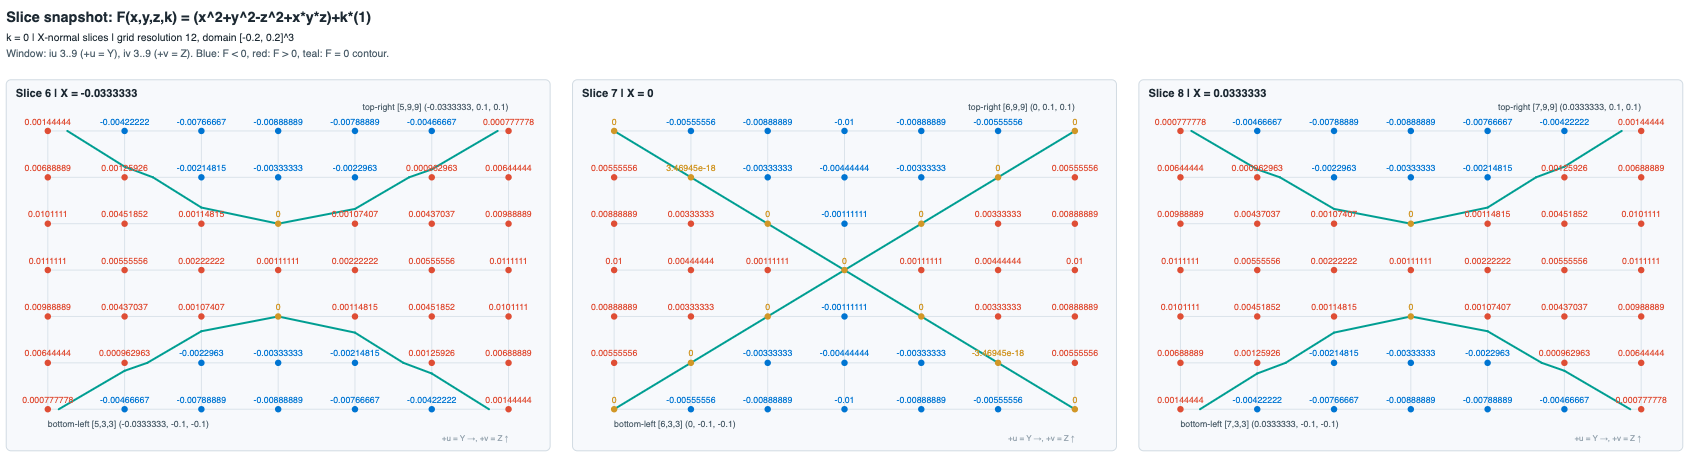
\includegraphics[width=\textwidth]{pictures/report/snap_A1_k0.png}\\[4pt]
    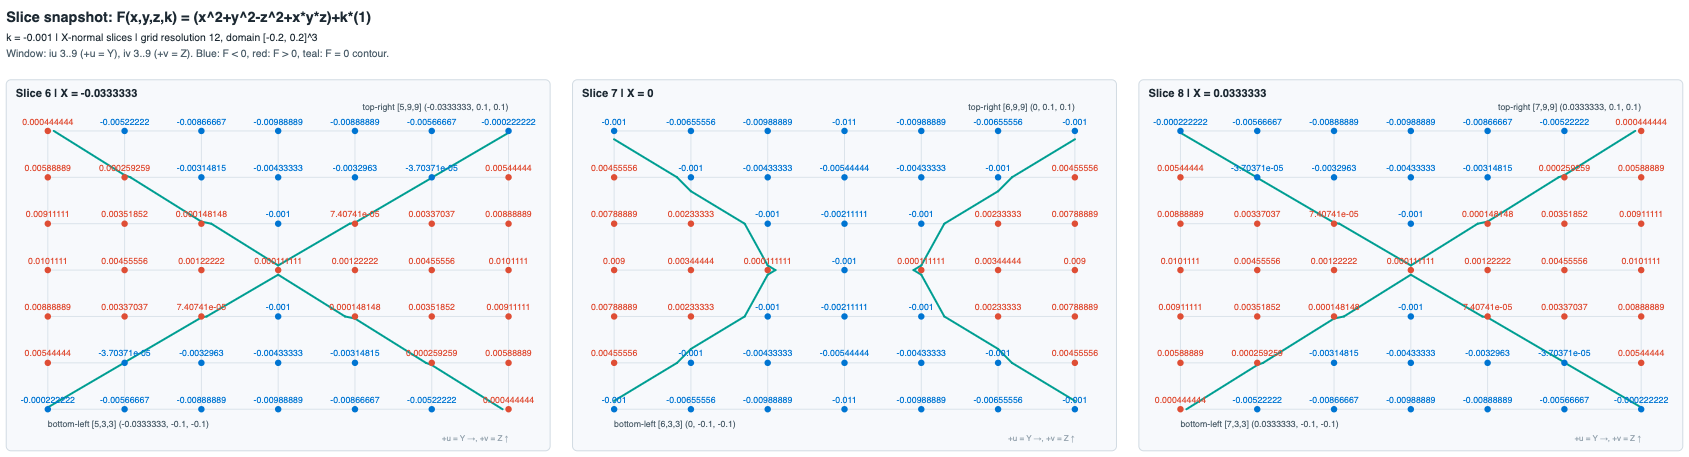
\includegraphics[width=\textwidth]{pictures/report/snap_A1_kneg.png}\\[4pt]
    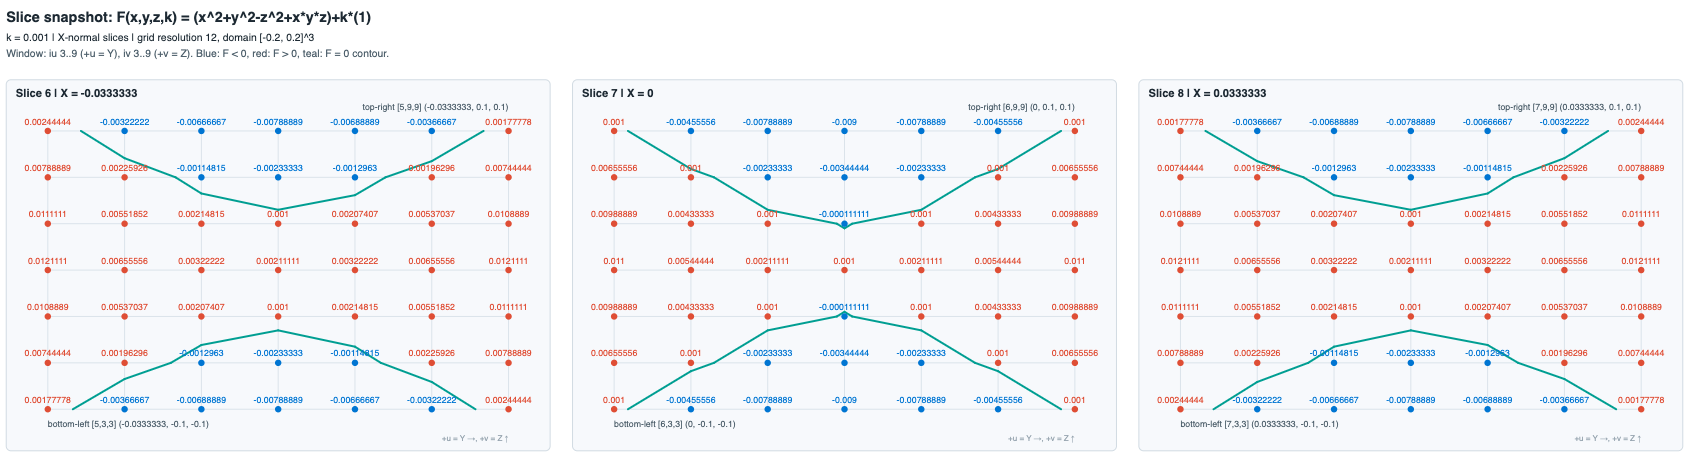
\includegraphics[width=\textwidth]{pictures/report/snap_A1_kpos.png}
    \caption{Slice snapshots around the singular point of $x^2+y^2-z^2+xyz+kG$ with $G=1$:
    $k=0$ (top), $k<0$ (middle), $k>0$ (bottom); the values of $k$, the grid and
    the window are printed in each snapshot. Every node shows its value (blue
    negative, red positive, yellow zero); teal is the zero level $S_k$.}
    \label{fig:r-A1-snap}
\end{figure}

\begin{table}[!h]
\centering
\footnotesize
\begin{adjustbox}{max width=\textwidth}
\begin{tabular}{l c l c c c c c c c}
\toprule
& & & & \multicolumn{2}{c}{$k<0$} & \multicolumn{2}{c}{$k>0$} & & \\
\cmidrule(lr){5-6}\cmidrule(lr){7-8}
$G$ & $m$ & essential part & predicted $\alpha$ & $\alpha$ & $C$ & $\alpha$ & $C$ & spread over $N$ & agrees \\
\midrule
$1$ & 0 & $1$ & $\tfrac12$ & 0.500{\scriptsize$\pm$0.000} & 1.00 & 0.500{\scriptsize$\pm$0.000} & 1.00 & 0.000 & yes \\
$x$ & 1 & $0$ & $1$ & 1.000{\scriptsize$\pm$0.000} & 0.71 & 1.000{\scriptsize$\pm$0.000} & 0.71 & 0.000 & yes \\
$y$ & 1 & $0$ & $1$ & 1.000{\scriptsize$\pm$0.000} & 0.71 & 1.000{\scriptsize$\pm$0.000} & 0.71 & 0.000 & yes \\
$z$ & 1 & $0$ & $1$ & 1.000{\scriptsize$\pm$0.000} & 0.71 & 1.000{\scriptsize$\pm$0.000} & 0.71 & 0.000 & yes \\
$x+y$ & 1 & $0$ & $1$ & 1.000{\scriptsize$\pm$0.001} & 1.00 & 1.000{\scriptsize$\pm$0.001} & 1.00 & 0.000 & yes \\
$x+z$ & 1 & $0$ & $1$ & 1.000{\scriptsize$\pm$0.000} & 0.71 & 1.000{\scriptsize$\pm$0.000} & 0.71 & 0.000 & yes \\
$x+y+z$ & 1 & $0$ & $1$ & 1.003{\scriptsize$\pm$0.004} & 1.01 & 1.003{\scriptsize$\pm$0.004} & 1.01 & 0.000 & yes \\
$2x-y+3z$ & 1 & $0$ & $1$ & 1.000{\scriptsize$\pm$0.001} & 2.12 & 1.000{\scriptsize$\pm$0.001} & 2.12 & 0.000 & yes \\
$x^2$ & 2 & $0$ & $1$ & 1.001{\scriptsize$\pm$0.000} & 0.06 & 0.999{\scriptsize$\pm$0.000} & 0.06 & 0.000 & yes \\
$x^2+y^2-z^2$ & 2 & $0$ & $1$ & 1.002{\scriptsize$\pm$0.001} & 0.01 & 0.998{\scriptsize$\pm$0.001} & 0.01 & 0.000 & yes \\
$xy$ & 2 & $0$ & $1$ & 1.000{\scriptsize$\pm$0.000} & 0.03 & 1.000{\scriptsize$\pm$0.000} & 0.03 & 0.000 & yes \\
$x^3$ & 3 & $0$ & $1$ & 1.000{\scriptsize$\pm$0.000} & 0.01 & 1.000{\scriptsize$\pm$0.000} & 0.01 & 0.000 & yes \\
$x^2y+y^2z+z^2x$ & 3 & $0$ & $1$ & 1.000{\scriptsize$\pm$0.000} & 0.02 & 1.000{\scriptsize$\pm$0.000} & 0.02 & 0.000 & yes \\
$F$ & -- & $0$ & $1$ & $S_k=S_0$ & -- & $S_k=S_0$ & -- & -- & yes \\
\bottomrule
\end{tabular}
\end{adjustbox}
\caption[Rates for $x^2+y^2-z^2+xyz$]{All perturbations of $F=x^2+y^2-z^2+xyz$: convergence rates (resolution $128$). Columns are explained in Section~\ref{sec:r-read}.}
\label{tab:r-A1-rates}
\end{table}
\begin{table}[!h]
\centering
\footnotesize
\begin{adjustbox}{max width=\textwidth}
\begin{tabular}{l l c l l c}
\toprule
$G$ & $P$ for $k\neq0$ & corank at $P$ & singular points, $k<0$ & singular points, $k>0$ & MC error \\
\midrule
$1$ & leaves $S_k$ & -- & none & none & 0.0010 \\
$x$ & regular & -- & none & none & 0.0025 \\
$y$ & regular & -- & none & none & 0.0025 \\
$z$ & regular & -- & none & none & 0.0024 \\
$x+y$ & regular & -- & none & none & 0.0036 \\
$x+z$ & regular & -- & none & none & 0.0022 \\
$x+y+z$ & regular & -- & none & none & 0.0035 \\
$2x-y+3z$ & regular & -- & none & none & 0.0020 \\
$x^2$ & singular & 0 ($A_1$) & only $P$ & only $P$ & 0.0014 \\
$x^2+y^2-z^2$ & singular & 0 ($A_1$) & only $P$ & only $P$ & 0.0014 \\
$xy$ & singular & 0 ($A_1$) & only $P$ & only $P$ & 0.0015 \\
$x^3$ & singular & 0 ($A_1$) & only $P$ & only $P$ & 0.0014 \\
$x^2y+y^2z+z^2x$ & singular & 0 ($A_1$) & only $P$ & only $P$ & 0.0013 \\
$F$ & singular & 0 ($A_1$) & only $P$ & only $P$ & 0.0014 \\
\bottomrule
\end{tabular}
\end{adjustbox}
\caption[Singular points for $x^2+y^2-z^2+xyz$]{All perturbations of $F=x^2+y^2-z^2+xyz$: the point $P$, the singular points of $S_k$ and the accuracy of Marching Cubes. Columns are explained in Section~\ref{sec:r-read}.}
\label{tab:r-A1-points}
\end{table}
\paragraph{Constant ($G=1$).} $G=1$ turns the double cone into a hyperboloid:
for $k<0$ the equation reads $x^2+y^2-z^2=|k|$ (one sheet with a narrow waist of
radius $\sqrt{|k|}$), for $k>0$ it reads $x^2+y^2-z^2=-k$ (two separate bowls with
tips at $z=\pm\sqrt k$). Either way the change happens at the distance $\sqrt{|k|}$
from the old tip, so $\alpha=\tfrac12$; the measured value is $0.500$ with $C=1.00$
on both sides. The snapshots (Figure~\ref{fig:r-A1-snap}) show the hyperbola on the
plane $x=0$: for $k<0$ the two branches open sideways, for $k>0$ up and down.

\paragraph{Linear $G$.} Every linear $G$ is inessential here, and all of them give
$\alpha=1.000$ (to $\pm0.003$) on both sides. The origin stays on the surface but
becomes regular. Completing the square shows why the rate is $1$: for example
$x^2+kx=(x+\tfrac k2)^2-\tfrac{k^2}{4}$, so the cone is \emph{shifted} by $k/2$ and
opened by the constant $-k^2/4$, which acts at the distance $\sqrt{k^2/4}=|k|/2$.
Both effects are proportional to $|k|$. The rate is the same for all linear $G$,
but the constant is not: $C=0.71$ for a single coordinate, $1.00$ for $x+y$ and
$2.12$ for $2x-y+3z$, because the shift grows with the coefficients of $G$.

\paragraph{Order two and three.} $P$ stays an ordinary double point (corank $0$ in
Table~\ref{tab:r-A1-points}). The cone is only bent, by a distance proportional to
$|k|$: $\alpha=1$, with small constants ($0.01$--$0.06$).

\paragraph{Singular points.} No perturbation creates a singular point other than
$P$. This agrees with $\mu=1$: there is only one stationary point near $P$ to begin
with.
\clearpage

\subsection{The cusp $x^2+y^2+z^3$}
\label{sec:r-A2a}

Near the origin the surface is $x^2+y^2=-z^3$: for each $z<0$ the
cross-section is a circle of radius $|z|^{3/2}$, and for $z>0$ there is nothing.
The surface is therefore a thin horn that ends in a sharp tip at the origin
(Figure~\ref{fig:r-A2a-exact}, slice $y=0$). The weights are
$(\tfrac12,\tfrac12,\tfrac13)$: shrinking $z$ by $t^{1/3}$ and $x,y$ by $t^{1/2}$
keeps the equation. The Tjurina basis is $\{1,z\}$: a constant and the $z$
direction are the only essential perturbations; $x$ and $y$ are inessential.


\begin{figure}[!h]
\centering
\begin{minipage}[c]{0.18\textwidth}\centering
      \centering
    \resizebox{\linewidth}{!}{\panel{exact_A2a_k0.png}} \\[2pt]
    {\footnotesize $k=0$}
\end{minipage}\hfill
\begin{minipage}[c]{0.72\textwidth}\centering
\begin{adjustbox}{max width=\textwidth}
\begin{tabular}{c c c}
$G$ & $k=-0.01$ & $k=+0.01$ \\
$1$ & \panel{exact_A2a_1_neg.png} & \panel{exact_A2a_1_pos.png} \\
$z$ & \panel{exact_A2a_z_neg.png} & \panel{exact_A2a_z_pos.png} \\
$x$ & \panel{exact_A2a_x_neg.png} & \panel{exact_A2a_x_pos.png} \\
\end{tabular}
\end{adjustbox}
\end{minipage}
\caption{Exact slices of $S_k$ on the plane $y=0$ (horizontal axis $x$, vertical
axis $z$, both from $-0.25$ to $0.25$), computed from the polynomial. Grey: the
singular surface $S_0$; blue: $S_k$; red: singular points of $S_k$ found by the
numerical stationary-point search; cross: the origin.}
\label{fig:r-A2a-exact}
\end{figure}

\begin{figure}[!h]
    \centering
    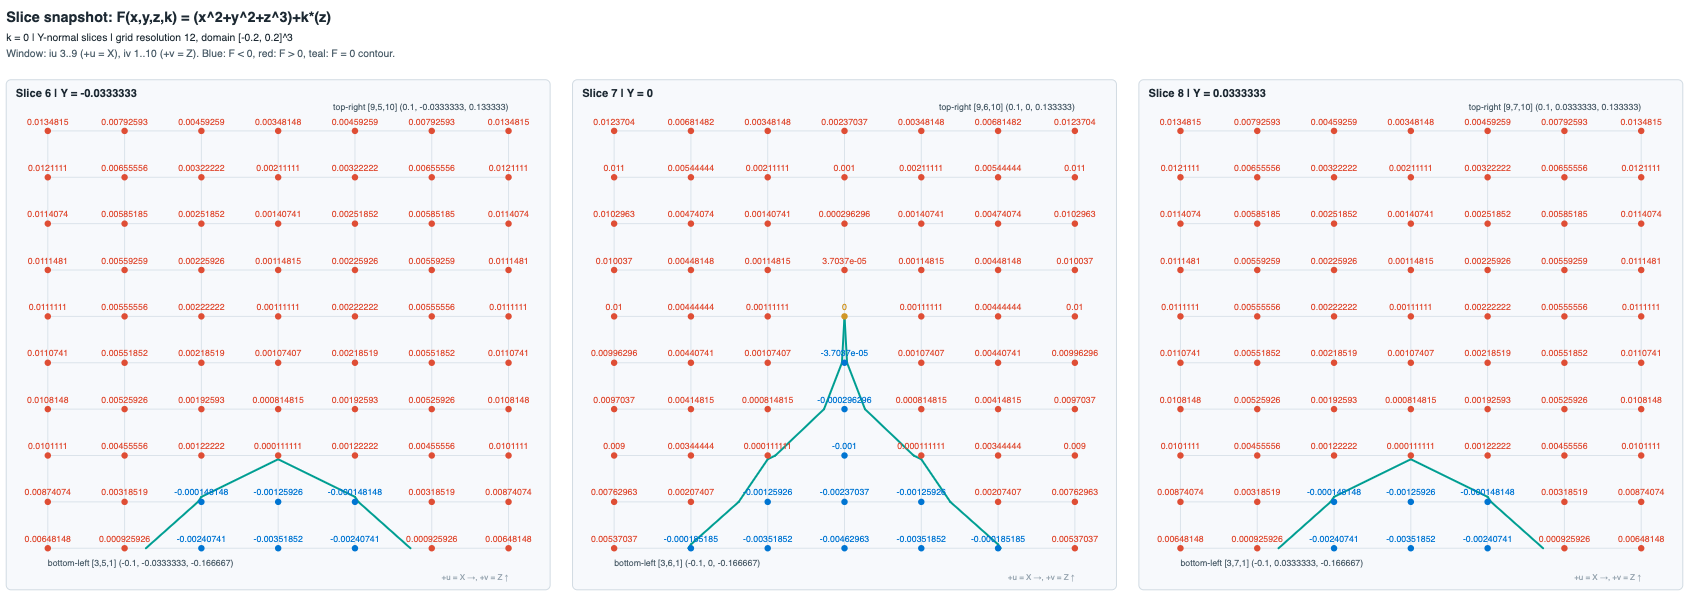
\includegraphics[width=\textwidth]{pictures/report/snap_A2a_k0.png}\\[4pt]
    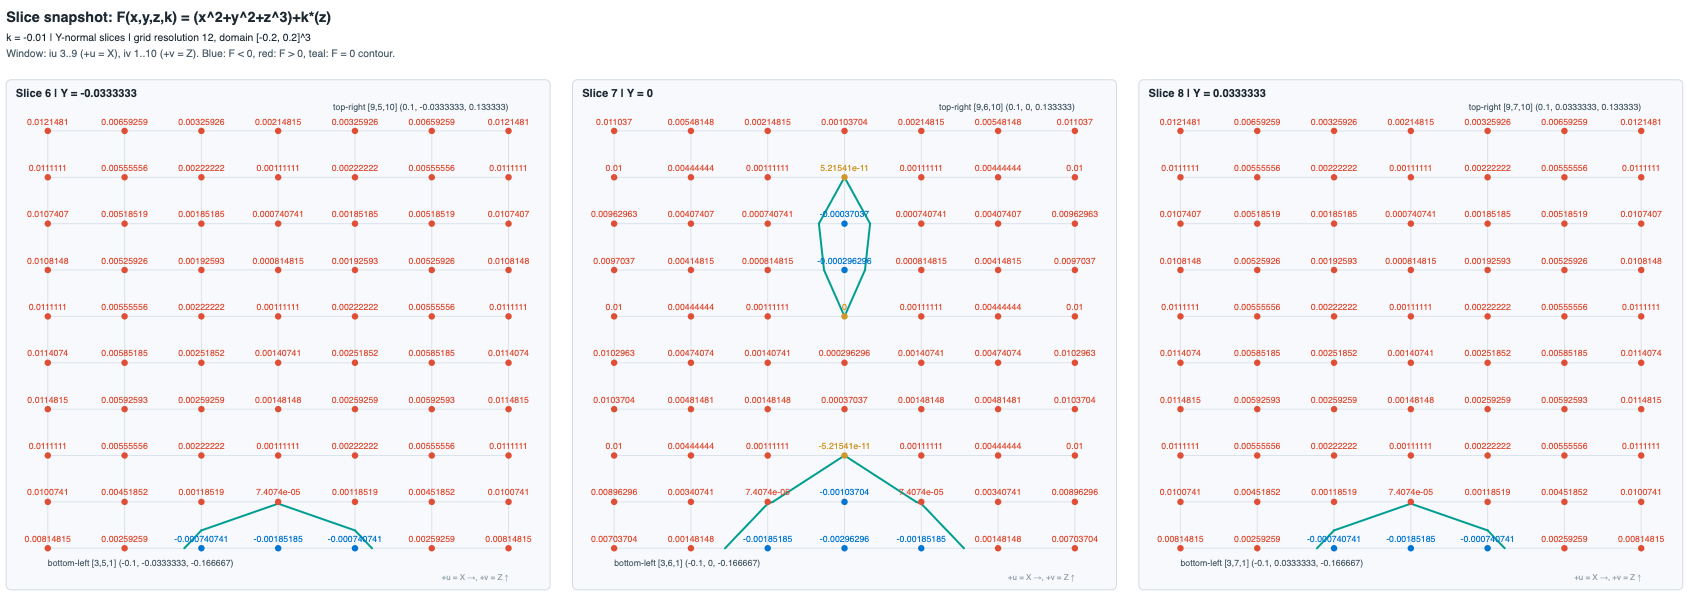
\includegraphics[width=\textwidth]{pictures/report/snap_A2a_kneg.png}\\[4pt]
    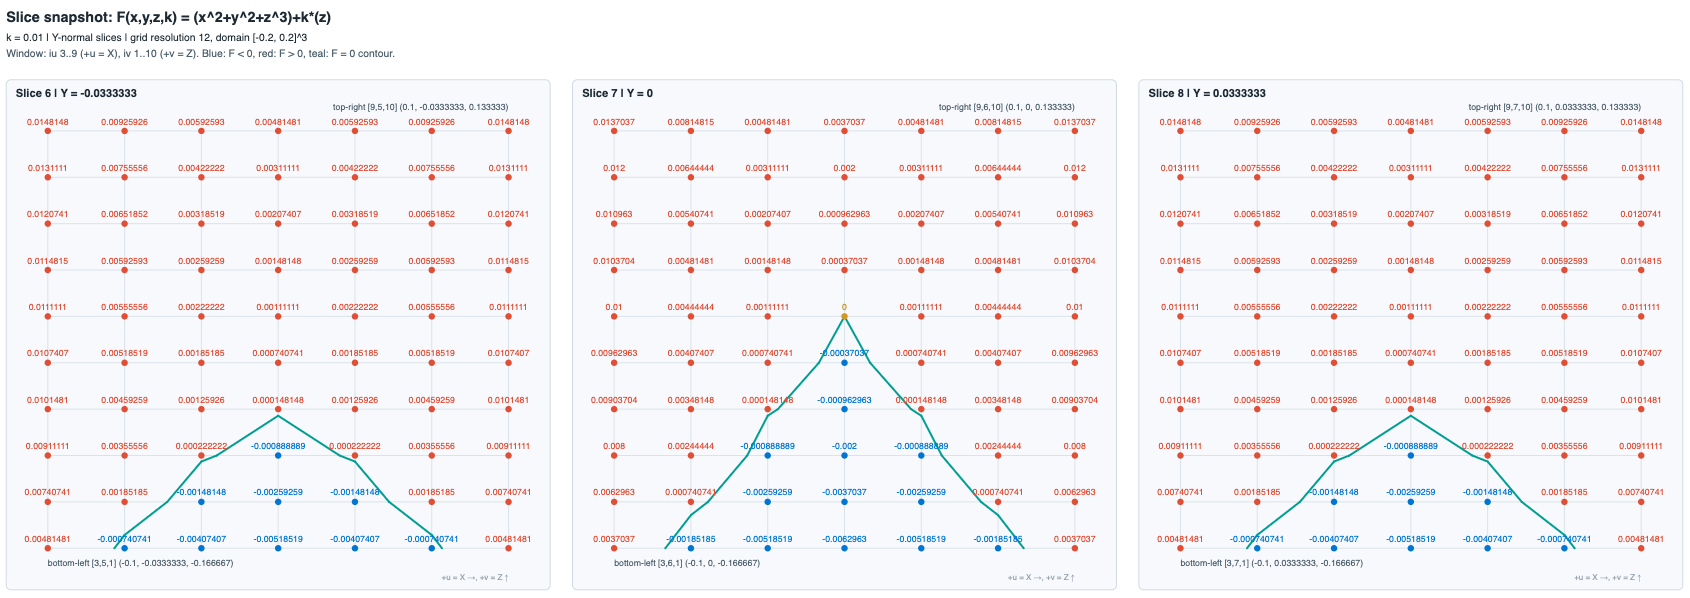
\includegraphics[width=\textwidth]{pictures/report/snap_A2a_kpos.png}
    \caption{Slice snapshots around the singular point of $x^2+y^2+z^3+kG$ with $G=z$:
    $k=0$ (top), $k<0$ (middle), $k>0$ (bottom); the values of $k$, the grid and
    the window are printed in each snapshot. Every node shows its value (blue
    negative, red positive, yellow zero); teal is the zero level $S_k$.}
    \label{fig:r-A2a-snap}
\end{figure}

\begin{table}[!h]
\centering
\footnotesize
\begin{adjustbox}{max width=\textwidth}
\begin{tabular}{l c l c c c c c c c}
\toprule
& & & & \multicolumn{2}{c}{$k<0$} & \multicolumn{2}{c}{$k>0$} & & \\
\cmidrule(lr){5-6}\cmidrule(lr){7-8}
$G$ & $m$ & essential part & predicted $\alpha$ & $\alpha$ & $C$ & $\alpha$ & $C$ & spread over $N$ & agrees \\
\midrule
$1$ & 0 & $1$ & $[\tfrac13,\tfrac12]$ & 0.341{\scriptsize$\pm$0.016} & 1.05 & 0.333{\scriptsize$\pm$0.000} & 1.00 & 0.044 & yes \\
$x$ & 1 & $0$ & $[\tfrac23,1]$ & 0.660{\scriptsize$\pm$0.026} & 0.59 & 0.660{\scriptsize$\pm$0.026} & 0.59 & 0.009 & yes \\
$y$ & 1 & $0$ & $[\tfrac23,1]$ & 0.660{\scriptsize$\pm$0.026} & 0.59 & 0.660{\scriptsize$\pm$0.026} & 0.59 & 0.009 & yes \\
$z$ & 1 & $z$ & $[\tfrac12,\tfrac34]$ & 0.500{\scriptsize$\pm$0.000} & 1.00 & 0.739{\scriptsize$\pm$0.003} & 0.40 & 0.000 & yes \\
$x+y$ & 1 & $0$ & $[\tfrac23,1]$ & 0.653{\scriptsize$\pm$0.051} & 0.70 & 0.653{\scriptsize$\pm$0.051} & 0.70 & 0.017 & yes \\
$x+z$ & 1 & $z$ & $[\tfrac12,\tfrac34]$ & 0.502{\scriptsize$\pm$0.001} & 1.02 & 0.787{\scriptsize$\pm$0.004} & 0.68 & 0.000 & \textbf{no} \\
$x+y+z$ & 1 & $z$ & $[\tfrac12,\tfrac34]$ & 0.505{\scriptsize$\pm$0.001} & 1.05 & 0.805{\scriptsize$\pm$0.006} & 0.83 & 0.000 & \textbf{no} \\
$2x-y+3z$ & 1 & $3z$ & $[\tfrac12,\tfrac34]$ & 0.502{\scriptsize$\pm$0.001} & 1.76 & 0.780{\scriptsize$\pm$0.002} & 1.44 & 0.000 & \textbf{no} \\
$x^2$ & 2 & $0$ & $1$ & 1.003{\scriptsize$\pm$0.002} & 0.03 & 0.999{\scriptsize$\pm$0.000} & 0.03 & 0.002 & yes \\
$x^2+y^2-z^2$ & 2 & $0$ & $1$ & 1.063{\scriptsize$\pm$0.044} & 0.71 & 1.000{\scriptsize$\pm$0.000} & 1.00 & 0.000 & yes \\
$xy$ & 2 & $0$ & $1$ & 1.001{\scriptsize$\pm$0.000} & 0.02 & 1.001{\scriptsize$\pm$0.000} & 0.02 & 0.000 & yes \\
$x^3$ & 3 & $0$ & $1$ & 1.000{\scriptsize$\pm$0.000} & 0.00 & 1.000{\scriptsize$\pm$0.000} & 0.00 & 0.000 & yes \\
$x^2y+y^2z+z^2x$ & 3 & $0$ & $1$ & 1.000{\scriptsize$\pm$0.000} & 0.01 & 1.000{\scriptsize$\pm$0.000} & 0.01 & 0.000 & yes \\
$F$ & -- & $0$ & $1$ & $S_k=S_0$ & -- & $S_k=S_0$ & -- & -- & yes \\
\bottomrule
\end{tabular}
\end{adjustbox}
\caption[Rates for $x^2+y^2+z^3$]{All perturbations of $F=x^2+y^2+z^3$: convergence rates (resolution $128$). Columns are explained in Section~\ref{sec:r-read}.}
\label{tab:r-A2a-rates}
\end{table}
\begin{table}[!h]
\centering
\footnotesize
\begin{adjustbox}{max width=\textwidth}
\begin{tabular}{l l c l l c}
\toprule
$G$ & $P$ for $k\neq0$ & corank at $P$ & singular points, $k<0$ & singular points, $k>0$ & MC error \\
\midrule
$1$ & leaves $S_k$ & -- & none & none & 0.0019 \\
$x$ & regular & -- & none & none & 0.0201 \\
$y$ & regular & -- & none & none & 0.0201 \\
$z$ & regular & -- & none & none & 0.0022 \\
$x+y$ & regular & -- & none & none & 0.0254 \\
$x+z$ & regular & -- & none & none & 0.0026 \\
$x+y+z$ & regular & -- & none & none & 0.0036 \\
$2x-y+3z$ & regular & -- & none & none & 0.0027 \\
$x^2$ & singular & 1 & only $P$ & only $P$ & 0.0021 \\
$x^2+y^2-z^2$ & singular & 0 ($A_1$) & only $P$ & only $P$ & 0.0080 \\
$xy$ & singular & 1 & only $P$ & only $P$ & 0.0021 \\
$x^3$ & singular & 1 & only $P$ & only $P$ & 0.0021 \\
$x^2y+y^2z+z^2x$ & singular & 1 & only $P$ & only $P$ & 0.0021 \\
$F$ & singular & 1 & only $P$ & only $P$ & 0.0021 \\
\bottomrule
\end{tabular}
\end{adjustbox}
\caption[Singular points for $x^2+y^2+z^3$]{All perturbations of $F=x^2+y^2+z^3$: the point $P$, the singular points of $S_k$ and the accuracy of Marching Cubes. Columns are explained in Section~\ref{sec:r-read}.}
\label{tab:r-A2a-points}
\end{table}
\paragraph{Constant ($G=1$).} $G=1$ moves the tip of the horn along the $z$-axis:
$x^2+y^2=-z^3-k$ has its tip at $z=-k^{1/3}$. The distance is $|k|^{1/3}$, the lower
end of the predicted range $[\tfrac13,\tfrac12]$; the measurement gives $0.341$
($k<0$) and $0.333$ ($k>0$) with $C\approx1$.

\paragraph{Linear $G$.} The essential direction $z$ behaves differently on the two
sides. For $k<0$ the cubic $z^3+kz$ gets two new real zeros $z=\pm\sqrt{|k|}$: the
horn \emph{splits open} along the axis over a length $\sqrt{|k|}$, so $\alpha=0.500$.
For $k>0$ there are no new zeros, the horn only gets thicker, and the change is
visible only across the axis, on the scale $|k|^{3/4}$: the measurement gives
$0.739$, the upper end $\tfrac34$ (Figure~\ref{fig:r-A2a-snap}).
The inessential directions $x$ and $y$ do not change the type of the singularity
but create a \emph{spike}: $(x+\tfrac k2)^2+y^2=\tfrac{k^2}{4}-z^3$ is the horn
shifted by $k/2$ plus a thin spike of radius about $|k|/2$ that reaches the height
$(k^2/4)^{1/3}$ above the old tip ($0.029$ for $|k|=0.01$;
Figure~\ref{fig:r-A2a-exact}, bottom row). Its height grows like $|k|^{2/3}$, and
the measured rate is $0.660$, the lower end $\tfrac23$.
The mixed perturbations $x+z$, $x+y+z$ and $2x-y+3z$ have the essential part $z$
(or $3z$) and behave like $z$ for $k<0$ ($0.50$). For $k>0$ they give $0.78$--$0.81$,
slightly above $\tfrac34$; these are the three ``no'' entries of
Table~\ref{tab:r-A2a-rates}. Their inessential part shifts the surface by a distance
proportional to $|k|$ (rate $1$) at the same time as the essential part acts with
rate $\tfrac34$; both effects are visible for $10^{-4}\le|k|\le10^{-2}$, so the
fitted slope lies between the two (Section~\ref{sec:r-deviations}).

\paragraph{Order two and three.} All of them keep the origin singular and give
$\alpha=1$. $G=x^2+y^2-z^2$ even makes the origin an ordinary double point
(corank $0$), because its term $-kz^2$ is stronger near the origin than $z^3$.

\paragraph{Singular points.} None other than $P$. The spike is so thin that
Marching Cubes misses it at every resolution: the extraction errors $0.0201$ for
$G=x$ and $G=y$ and $0.0254$ for $G=x+y$ in Table~\ref{tab:r-A2a-points} (three to
four grid cells, several times more than for the other perturbations) are the part
of the spike that is missing from the mesh.
\clearpage

\subsection{The cusp with a saddle: $x^2-y^2+z^3$}
\label{sec:r-A2b}

Over the complex numbers this is the same singularity as the previous one
($A_2$, $\mu=2$, basis $\{1,z\}$), but over the real numbers it looks different:
the quadratic part $x^2-y^2$ is a saddle, not a bowl. On the plane $z=0$ the
surface is the pair of lines $x=\pm y$; the cubic term bends these two sheets
into each other along the $z$-axis. The comparison with $x^2+y^2+z^3$ shows how
much the real geometry (the signs) matters, even when the algebraic type is the
same.

\begin{figure}[!h]
\centering
\begin{minipage}[c]{0.18\textwidth}\centering
      \centering
    \resizebox{\linewidth}{!}{\panel{exact_A2b_k0.png}} \\[2pt]
    {\footnotesize $k=0$}
\end{minipage}\hfill
\begin{minipage}[c]{0.72\textwidth}\centering
\begin{adjustbox}{max width=\textwidth}
\begin{tabular}{c c c}
$G$ & $k=-0.01$ & $k=+0.01$ \\
$1$ & \panel{exact_A2b_1_neg.png} & \panel{exact_A2b_1_pos.png} \\
$x+y$ & \panel{exact_A2b_xpy_neg.png} & \panel{exact_A2b_xpy_pos.png} \\
$z$ & \panel{exact_A2b_z_neg.png} & \panel{exact_A2b_z_pos.png} \\
\end{tabular}
\end{adjustbox}
\end{minipage}
\caption{Exact slices of $S_k$ on the plane $z=0$ (horizontal axis $x$, vertical
axis $y$, both from $-0.25$ to $0.25$), computed from the polynomial. Grey: the
singular surface $S_0$; blue: $S_k$; red: singular points of $S_k$ found by the
numerical stationary-point search; cross: the origin.}
\label{fig:r-A2b-exact}
\end{figure}

\begin{figure}[!h]
    \centering
    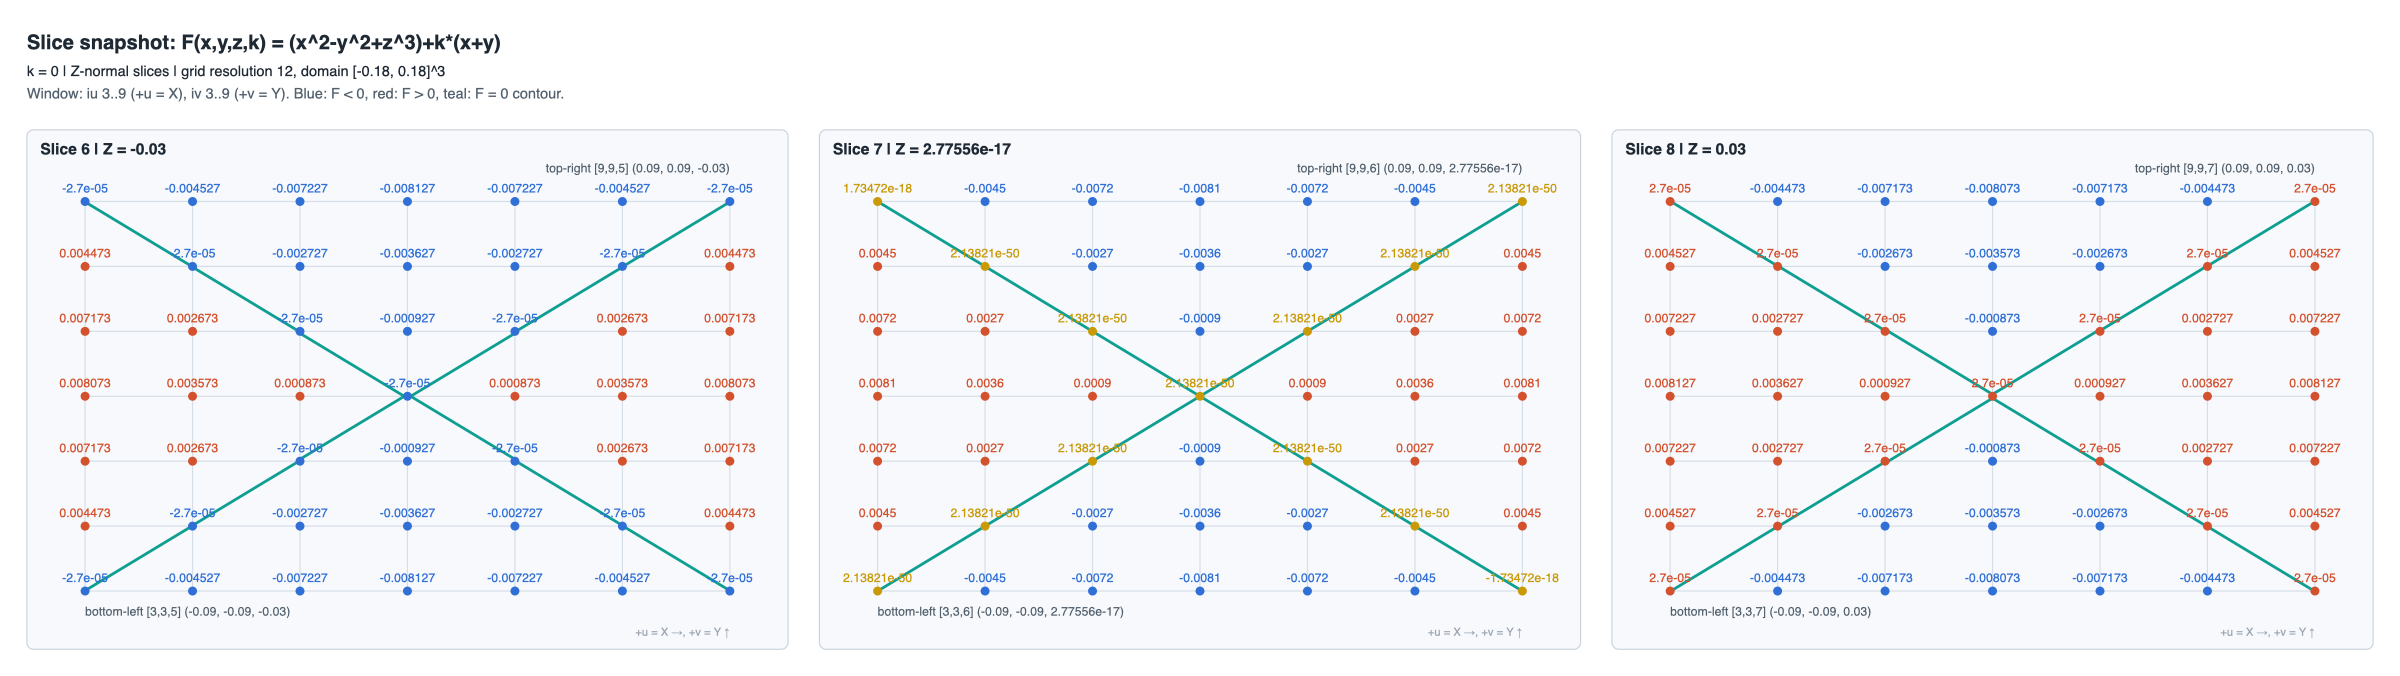
\includegraphics[width=\textwidth]{pictures/report/snap_A2b_k0.png}\\[4pt]
    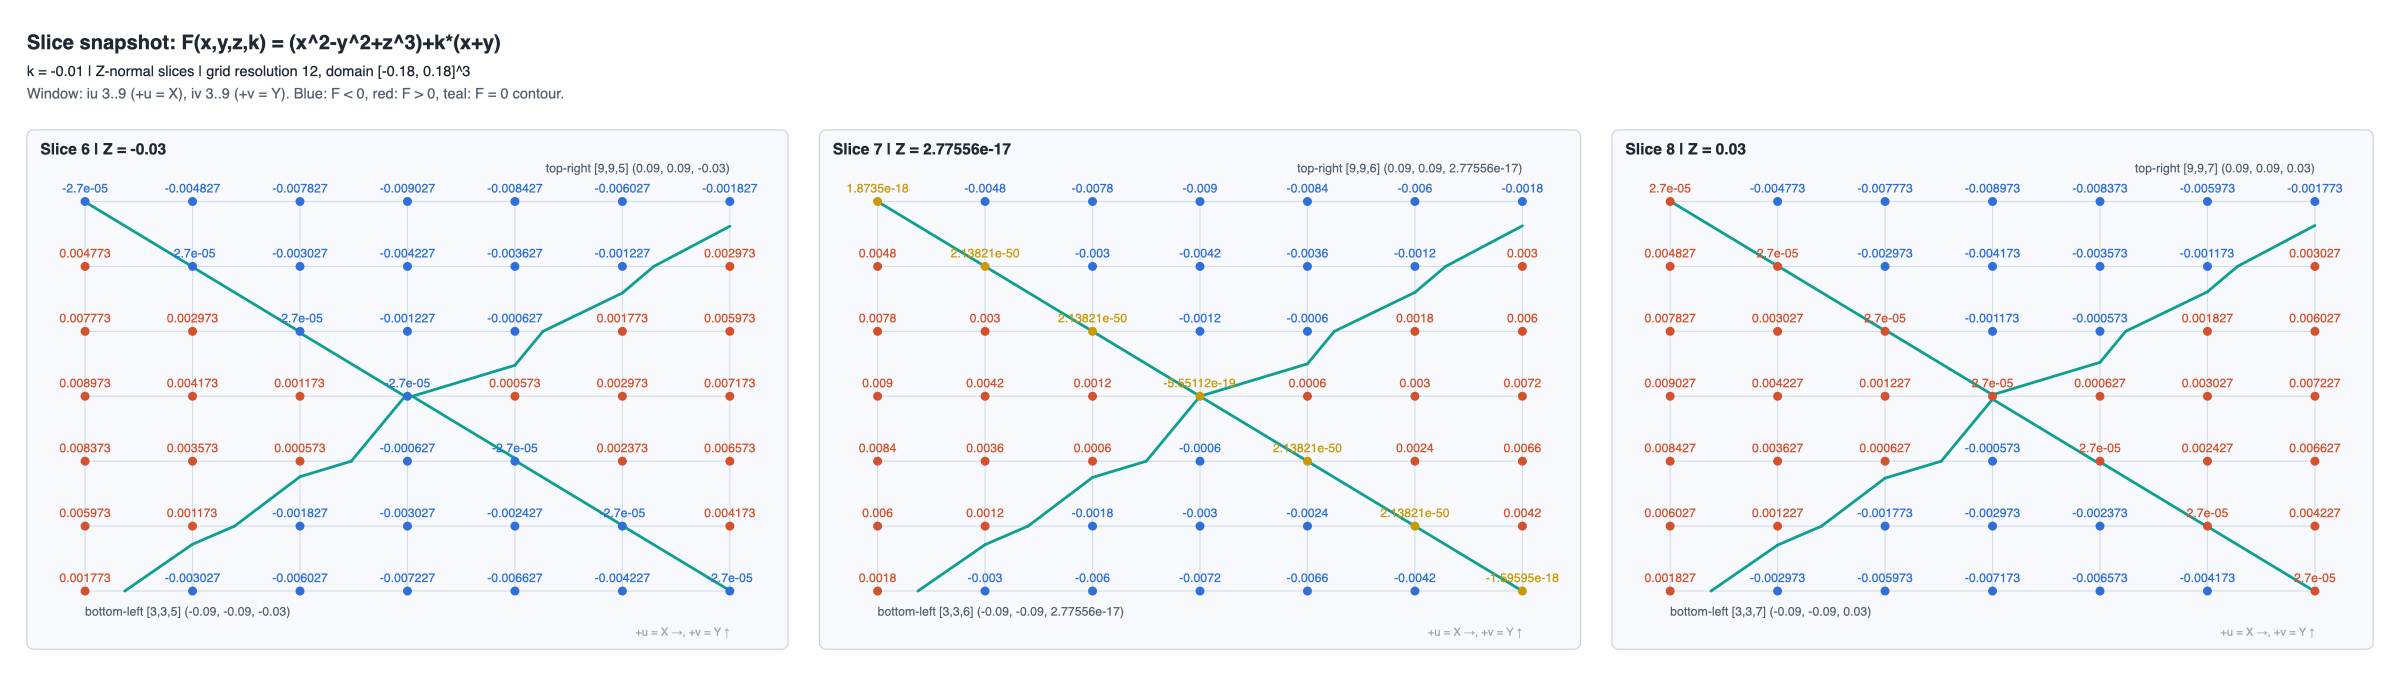
\includegraphics[width=\textwidth]{pictures/report/snap_A2b_kneg.png}\\[4pt]
    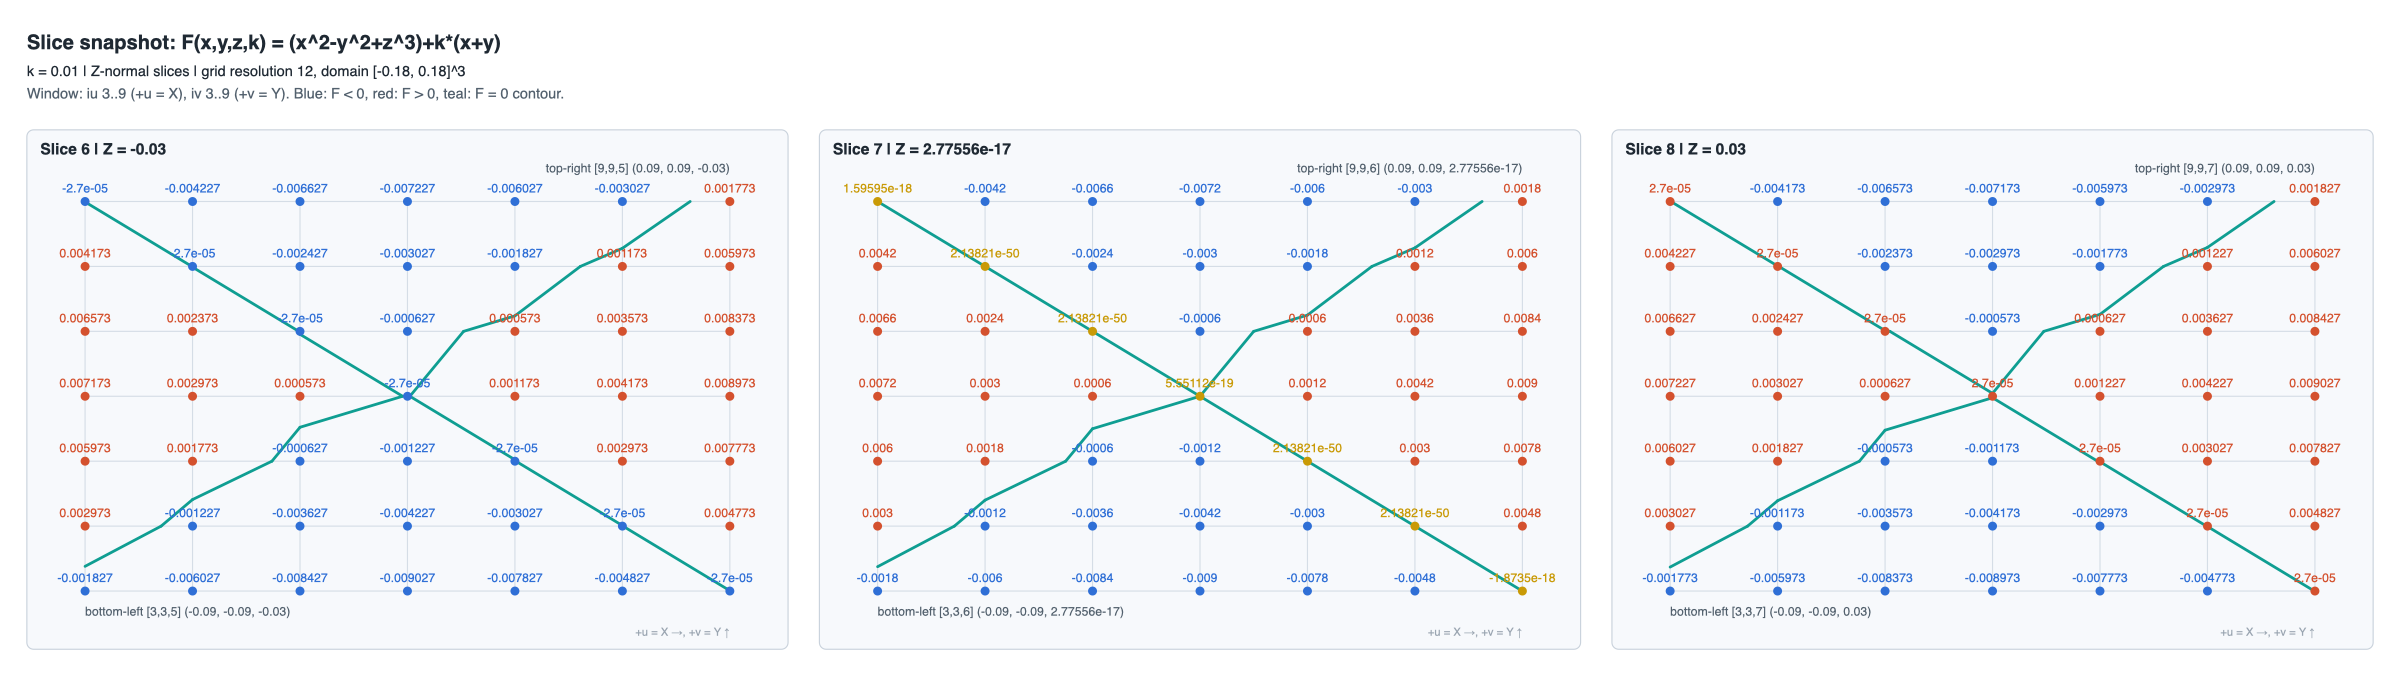
\includegraphics[width=\textwidth]{pictures/report/snap_A2b_kpos.png}
    \caption{Slice snapshots around the singular point of $x^2-y^2+z^3+kG$ with $G=x+y$:
    $k=0$ (top), $k<0$ (middle), $k>0$ (bottom); the values of $k$, the grid and
    the window are printed in each snapshot. Every node shows its value (blue
    negative, red positive, yellow zero); teal is the zero level $S_k$.}
    \label{fig:r-A2b-snap}
\end{figure}

\begin{table}[!h]
\centering
\footnotesize
\begin{adjustbox}{max width=\textwidth}
\begin{tabular}{l c l c c c c c c c}
\toprule
& & & & \multicolumn{2}{c}{$k<0$} & \multicolumn{2}{c}{$k>0$} & & \\
\cmidrule(lr){5-6}\cmidrule(lr){7-8}
$G$ & $m$ & essential part & predicted $\alpha$ & $\alpha$ & $C$ & $\alpha$ & $C$ & spread over $N$ & agrees \\
\midrule
$1$ & 0 & $1$ & $[\tfrac13,\tfrac12]$ & 0.500{\scriptsize$\pm$0.000} & 1.00 & 0.500{\scriptsize$\pm$0.000} & 1.00 & 0.000 & yes \\
$x$ & 1 & $0$ & $[\tfrac23,1]$ & 0.932{\scriptsize$\pm$0.111} & 0.49 & 0.932{\scriptsize$\pm$0.111} & 0.49 & 0.038 & yes \\
$y$ & 1 & $0$ & $[\tfrac23,1]$ & 0.932{\scriptsize$\pm$0.110} & 0.49 & 0.932{\scriptsize$\pm$0.110} & 0.49 & 0.068 & yes \\
$z$ & 1 & $z$ & $[\tfrac12,\tfrac34]$ & 0.732{\scriptsize$\pm$0.004} & 0.85 & 0.739{\scriptsize$\pm$0.003} & 0.40 & 0.000 & yes \\
$x+y$ & 1 & $0$ & $[\tfrac23,1]$ & 0.985{\scriptsize$\pm$0.046} & 0.66 & 0.980{\scriptsize$\pm$0.050} & 0.64 & 0.009 & yes \\
$x+z$ & 1 & $z$ & $[\tfrac12,\tfrac34]$ & 0.738{\scriptsize$\pm$0.003} & 0.89 & 0.787{\scriptsize$\pm$0.004} & 0.68 & 0.001 & \textbf{no} \\
$x+y+z$ & 1 & $z$ & $[\tfrac12,\tfrac34]$ & 0.742{\scriptsize$\pm$0.009} & 0.90 & 0.786{\scriptsize$\pm$0.004} & 0.67 & 0.005 & \textbf{no} \\
$2x-y+3z$ & 1 & $3z$ & $[\tfrac12,\tfrac34]$ & 0.728{\scriptsize$\pm$0.004} & 1.84 & 0.775{\scriptsize$\pm$0.002} & 1.36 & 0.003 & \textbf{no} \\
$x^2$ & 2 & $0$ & $1$ & 1.001{\scriptsize$\pm$0.000} & 0.07 & 0.999{\scriptsize$\pm$0.000} & 0.06 & 0.002 & yes \\
$x^2+y^2-z^2$ & 2 & $0$ & $1$ & 1.004{\scriptsize$\pm$0.002} & 0.15 & 1.004{\scriptsize$\pm$0.002} & 0.15 & 0.000 & yes \\
$xy$ & 2 & $0$ & $1$ & 1.000{\scriptsize$\pm$0.000} & 0.06 & 1.000{\scriptsize$\pm$0.000} & 0.06 & 0.001 & yes \\
$x^3$ & 3 & $0$ & $1$ & 1.000{\scriptsize$\pm$0.000} & 0.01 & 1.000{\scriptsize$\pm$0.000} & 0.01 & 0.003 & yes \\
$x^2y+y^2z+z^2x$ & 3 & $0$ & $1$ & 1.000{\scriptsize$\pm$0.000} & 0.03 & 1.000{\scriptsize$\pm$0.000} & 0.03 & 0.000 & yes \\
$F$ & -- & $0$ & $1$ & $S_k=S_0$ & -- & $S_k=S_0$ & -- & -- & yes \\
\bottomrule
\end{tabular}
\end{adjustbox}
\caption[Rates for $x^2-y^2+z^3$]{All perturbations of $F=x^2-y^2+z^3$: convergence rates (resolution $128$). Columns are explained in Section~\ref{sec:r-read}.}
\label{tab:r-A2b-rates}
\end{table}
\begin{table}[!h]
\centering
\footnotesize
\begin{adjustbox}{max width=\textwidth}
\begin{tabular}{l l c l l c}
\toprule
$G$ & $P$ for $k\neq0$ & corank at $P$ & singular points, $k<0$ & singular points, $k>0$ & MC error \\
\midrule
$1$ & leaves $S_k$ & -- & none & none & 0.0011 \\
$x$ & regular & -- & none & none & 0.0029 \\
$y$ & regular & -- & none & none & 0.0029 \\
$z$ & regular & -- & none & none & 0.0016 \\
$x+y$ & regular & -- & 1$\times$$A_2$, $\gamma=1.00$ & 1$\times$$A_2$, $\gamma=1.00$ & 0.0023 \\
$x+z$ & regular & -- & none & none & 0.0023 \\
$x+y+z$ & regular & -- & none & none & 0.0021 \\
$2x-y+3z$ & regular & -- & none & none & 0.0020 \\
$x^2$ & singular & 1 & only $P$ & only $P$ & 0.0015 \\
$x^2+y^2-z^2$ & singular & 0 ($A_1$) & only $P$ & only $P$ & 0.0015 \\
$xy$ & singular & 1 & only $P$ & only $P$ & 0.0015 \\
$x^3$ & singular & 1 & only $P$ & only $P$ & 0.0015 \\
$x^2y+y^2z+z^2x$ & singular & 1 & only $P$ & only $P$ & 0.0015 \\
$F$ & singular & 1 & only $P$ & only $P$ & 0.0015 \\
\bottomrule
\end{tabular}
\end{adjustbox}
\caption[Singular points for $x^2-y^2+z^3$]{All perturbations of $F=x^2-y^2+z^3$: the point $P$, the singular points of $S_k$ and the accuracy of Marching Cubes. Columns are explained in Section~\ref{sec:r-read}.}
\label{tab:r-A2b-points}
\end{table}
\paragraph{Constant ($G=1$).} $G=1$ turns the pair of lines $x=\pm y$ into the
hyperbola $x^2-y^2=-k$, which is $\sqrt{|k|}$ away from the crossing: $\alpha=0.500$ on
both sides, the \emph{upper} end of the range, while the horn of $x^2+y^2+z^3$ gave
the lower end $\tfrac13$. The horn can only move along its axis; the saddle opens
across it.

\paragraph{Linear $G$.} The essential direction $z$ gives $0.73$--$0.74$ on both
sides, close to the upper end $\tfrac34$: the saddle removes the difference between
the sides that the horn had. The inessential $x$ and $y$ give $0.93$ instead of
$0.66$: there is no spike, because the saddle has no tube for a spike to sit in, and
the shift by $k/2$ (rate $1$) dominates. The mixed $x+z$, $x+y+z$ and $2x-y+3z$ give
$0.73$--$0.79$; their values for $k>0$ ($0.78$--$0.79$) are just above $\tfrac34$,
which gives the three ``no'' entries of Table~\ref{tab:r-A2b-rates}, for the same
reason as for $x^2+y^2+z^3$.

\paragraph{Order two and three.} The origin stays singular (corank $1$; corank $0$
for $x^2+y^2-z^2$) and $\alpha=1$.

\paragraph{Singular points.} Only $G=x+y$ creates one, and it does so in a special
way: $x^2-y^2+k(x+y)=(x+y)(x-y+k)$, so $S_k$ is the same pair of planes, one of them
shifted by $k$, bent by $z^3$. The cusp is not opened but \emph{moved} to
$(-\tfrac k2,\tfrac k2,0)$, and the numerical stationary-point search finds exactly
one $A_2$ point there for every $k$, moving with $\gamma=1.00$. The snapshots of
Figure~\ref{fig:r-A2b-snap} show the two lines crossing at the origin for $k=0$; for
$k=\pm0.01$ the crossing moves by $k/2$ in $x$ and $y$, a sixth of a grid cell, so on
the grid it looks almost unchanged although $P$ is no longer singular.
\clearpage

\subsection{The cusp in a different direction: $x^3+y^3+z^2+x^2$}
\label{sec:r-A2c}

Near the origin $x^2(1+x)+z^2+y^3$ is $x^2+z^2+y^3$ after the substitution
$\tilde x=x\sqrt{1+x}$: the same horn as $x^2+y^2+z^3$, but pointing along the
$y$-axis instead of $z$. The term $x^3$ only matters far from the origin. The
weights are $(\tfrac12,\tfrac13,\tfrac12)$ and the basis is $\{1,y\}$.

\begin{figure}[!h]
\centering
\begin{minipage}[c]{0.18\textwidth}\centering
      \centering
    \resizebox{\linewidth}{!}{\panel{exact_A2c_k0.png}} \\[2pt]
    {\footnotesize $k=0$}
\end{minipage}\hfill
\begin{minipage}[c]{0.72\textwidth}\centering
\begin{adjustbox}{max width=\textwidth}
\begin{tabular}{c c c}
$G$ & $k=-0.01$ & $k=+0.01$ \\
$1$ & \panel{exact_A2c_1_neg.png} & \panel{exact_A2c_1_pos.png} \\
$y$ & \panel{exact_A2c_y_neg.png} & \panel{exact_A2c_y_pos.png} \\
$x+z$ & \panel{exact_A2c_xpz_neg.png} & \panel{exact_A2c_xpz_pos.png} \\
\end{tabular}
\end{adjustbox}
\end{minipage}
\caption{Exact slices of $S_k$ on the plane $x=0$ (horizontal axis $y$, vertical
axis $z$, both from $-0.25$ to $0.25$), computed from the polynomial. Grey: the
singular surface $S_0$; blue: $S_k$; red: singular points of $S_k$ found by the
numerical stationary-point search; cross: the origin.}
\label{fig:r-A2c-exact}
\end{figure}

\begin{figure}[!h]
    \centering
    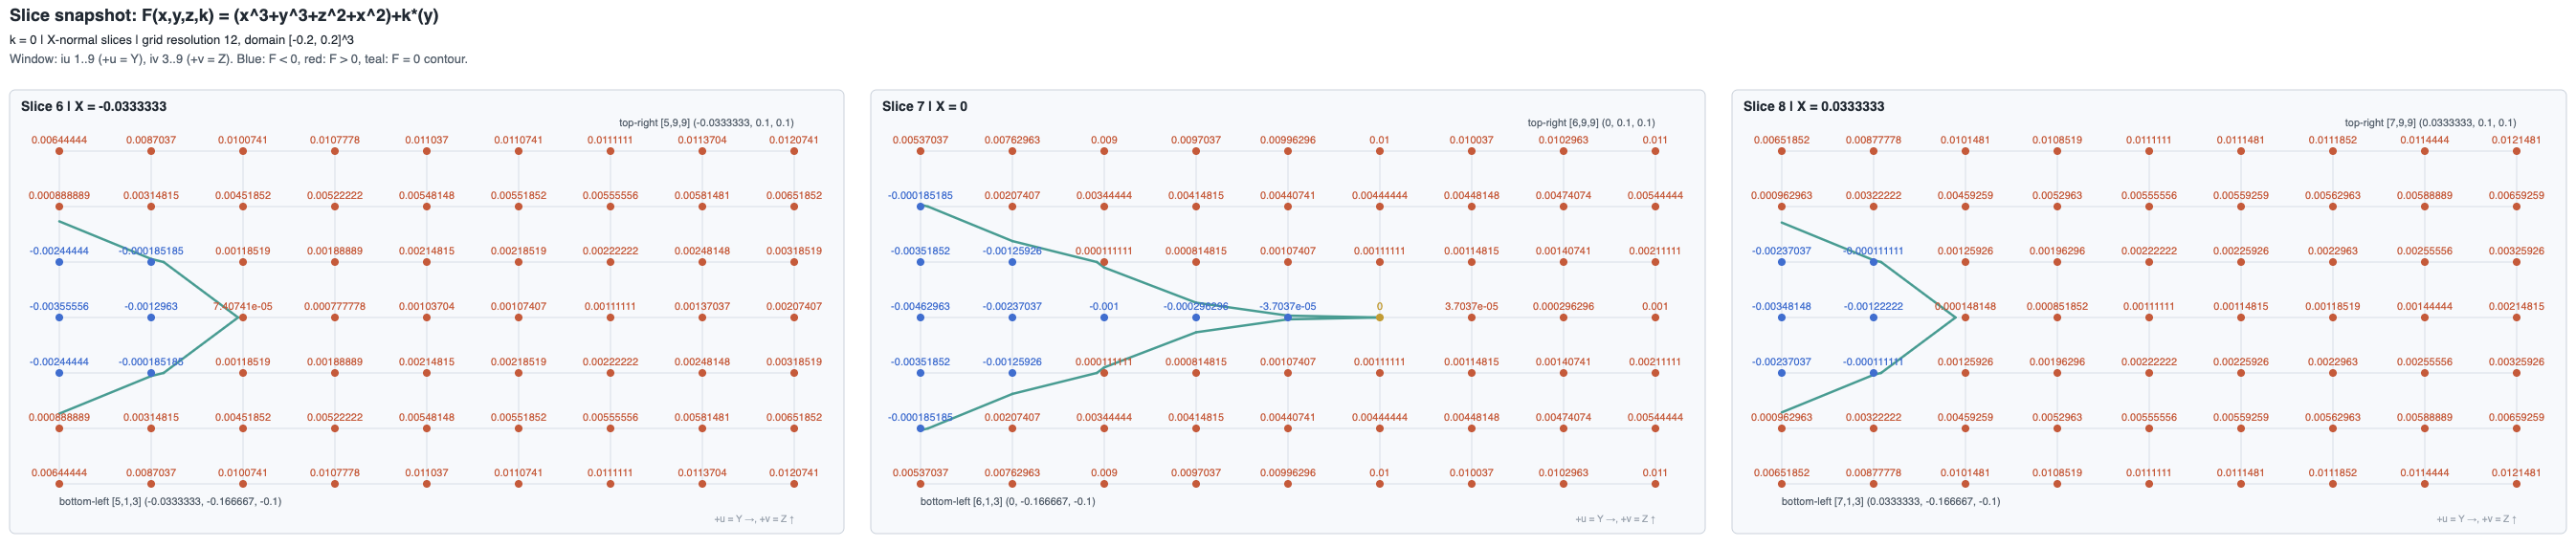
\includegraphics[width=\textwidth]{pictures/report/snap_A2c_k0.png}\\[4pt]
    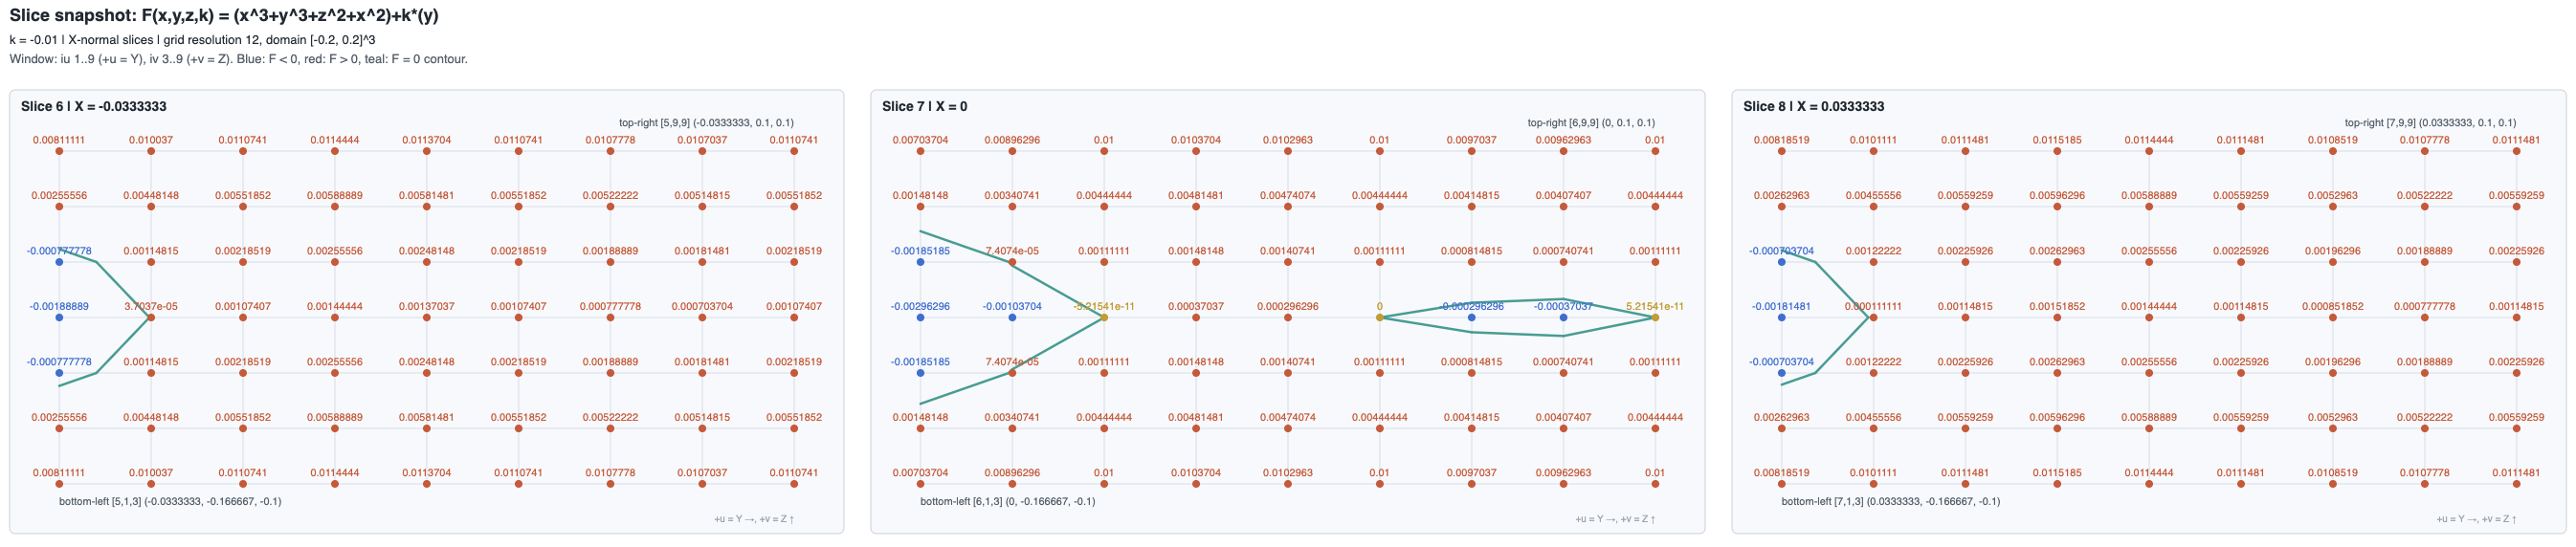
\includegraphics[width=\textwidth]{pictures/report/snap_A2c_kneg.png}\\[4pt]
    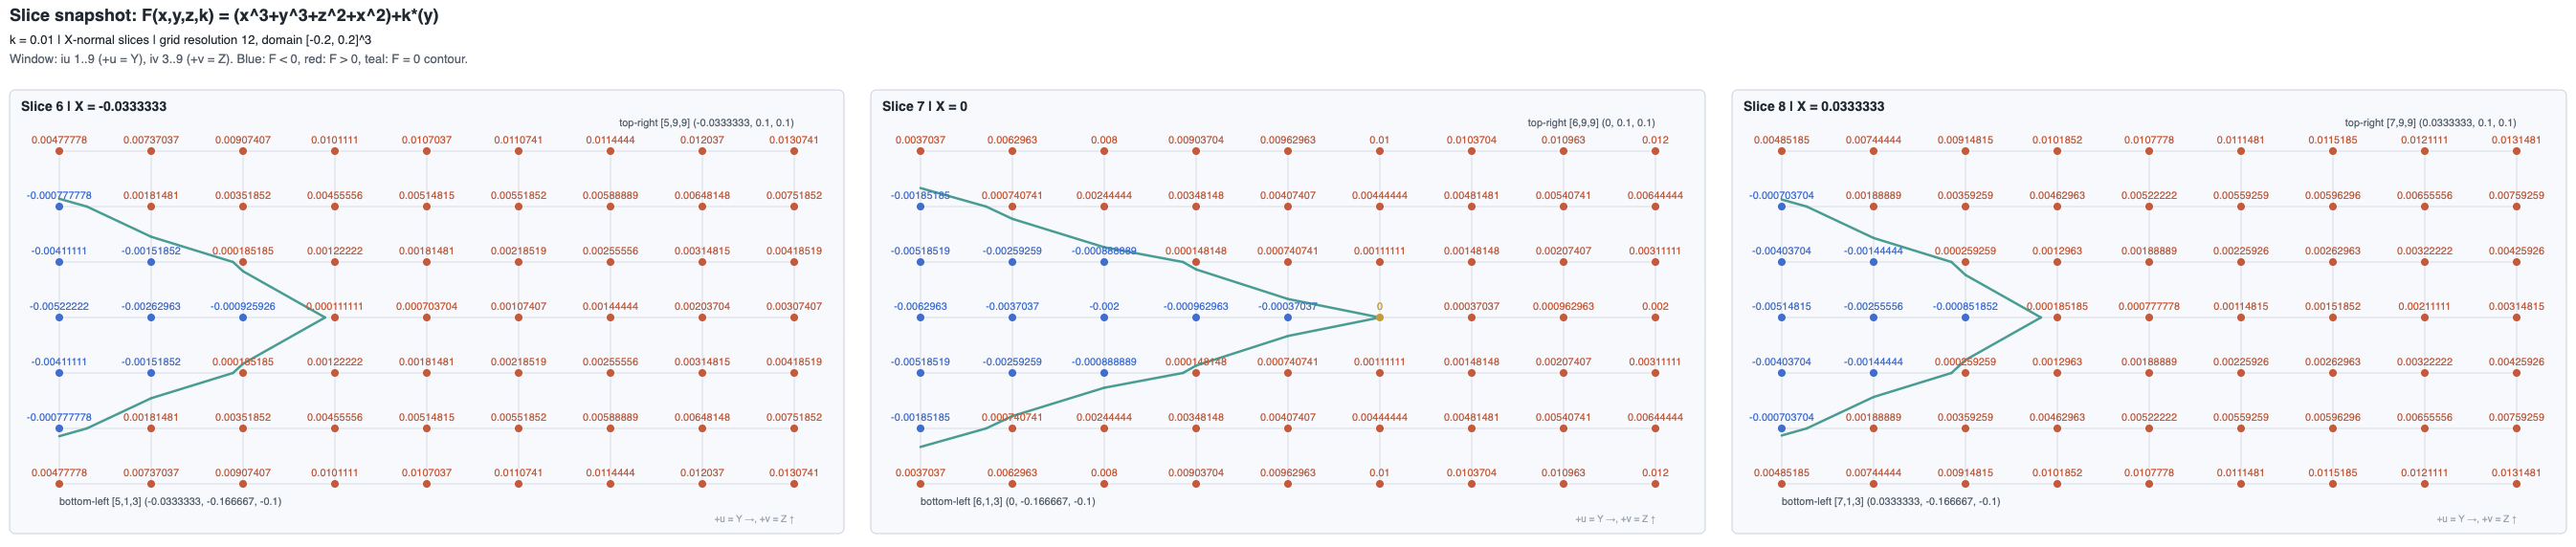
\includegraphics[width=\textwidth]{pictures/report/snap_A2c_kpos.png}
    \caption{Slice snapshots around the singular point of $x^3+y^3+z^2+x^2+kG$ with $G=y$:
    $k=0$ (top), $k<0$ (middle), $k>0$ (bottom); the values of $k$, the grid and
    the window are printed in each snapshot. Every node shows its value (blue
    negative, red positive, yellow zero); teal is the zero level $S_k$.}
    \label{fig:r-A2c-snap}
\end{figure}

\begin{table}[!h]
\centering
\footnotesize
\begin{adjustbox}{max width=\textwidth}
\begin{tabular}{l c l c c c c c c c}
\toprule
& & & & \multicolumn{2}{c}{$k<0$} & \multicolumn{2}{c}{$k>0$} & & \\
\cmidrule(lr){5-6}\cmidrule(lr){7-8}
$G$ & $m$ & essential part & predicted $\alpha$ & $\alpha$ & $C$ & $\alpha$ & $C$ & spread over $N$ & agrees \\
\midrule
$1$ & 0 & $1$ & $[\tfrac13,\tfrac12]$ & 0.341{\scriptsize$\pm$0.016} & 1.05 & 0.333{\scriptsize$\pm$0.000} & 1.00 & 0.043 & yes \\
$x$ & 1 & $0$ & $[\tfrac23,1]$ & 0.659{\scriptsize$\pm$0.030} & 0.59 & 0.666{\scriptsize$\pm$0.010} & 0.62 & 0.010 & yes \\
$y$ & 1 & $y$ & $[\tfrac12,\tfrac34]$ & 0.500{\scriptsize$\pm$0.000} & 1.00 & 0.742{\scriptsize$\pm$0.002} & 0.41 & 0.000 & yes \\
$z$ & 1 & $0$ & $[\tfrac23,1]$ & 0.660{\scriptsize$\pm$0.026} & 0.59 & 0.660{\scriptsize$\pm$0.026} & 0.59 & 0.009 & yes \\
$x+y$ & 1 & $y$ & $[\tfrac12,\tfrac34]$ & 0.502{\scriptsize$\pm$0.001} & 1.02 & 0.792{\scriptsize$\pm$0.006} & 0.71 & 0.000 & \textbf{no} \\
$x+z$ & 1 & $0$ & $[\tfrac23,1]$ & 0.653{\scriptsize$\pm$0.051} & 0.70 & 0.653{\scriptsize$\pm$0.050} & 0.70 & 0.017 & yes \\
$x+y+z$ & 1 & $y$ & $[\tfrac12,\tfrac34]$ & 0.505{\scriptsize$\pm$0.001} & 1.05 & 0.807{\scriptsize$\pm$0.007} & 0.85 & 0.000 & \textbf{no} \\
$2x-y+3z$ & 1 & $-y$ & $[\tfrac12,\tfrac34]$ & 0.883{\scriptsize$\pm$0.014} & 2.08 & 0.522{\scriptsize$\pm$0.006} & 1.23 & 0.000 & \textbf{no} \\
$x^2$ & 2 & $0$ & $1$ & 1.002{\scriptsize$\pm$0.001} & 0.04 & 0.999{\scriptsize$\pm$0.001} & 0.04 & 0.000 & yes \\
$x^2+y^2-z^2$ & 2 & $0$ & $1$ & 1.000{\scriptsize$\pm$0.000} & 1.00 & 1.063{\scriptsize$\pm$0.044} & 0.71 & 0.000 & yes \\
$xy$ & 2 & $0$ & $1$ & 1.001{\scriptsize$\pm$0.001} & 0.08 & 0.999{\scriptsize$\pm$0.000} & 0.08 & 0.000 & yes \\
$x^3$ & 3 & $0$ & $1$ & 1.000{\scriptsize$\pm$0.000} & 0.00 & 1.000{\scriptsize$\pm$0.000} & 0.00 & 0.000 & yes \\
$x^2y+y^2z+z^2x$ & 3 & $0$ & $1$ & 1.000{\scriptsize$\pm$0.000} & 0.01 & 1.000{\scriptsize$\pm$0.000} & 0.01 & 0.000 & yes \\
$F$ & -- & $0$ & $1$ & $S_k=S_0$ & -- & $S_k=S_0$ & -- & -- & yes \\
\bottomrule
\end{tabular}
\end{adjustbox}
\caption[Rates for $x^3+y^3+z^2+x^2$]{All perturbations of $F=x^3+y^3+z^2+x^2$: convergence rates (resolution $128$). Columns are explained in Section~\ref{sec:r-read}.}
\label{tab:r-A2c-rates}
\end{table}
\begin{table}[!h]
\centering
\footnotesize
\begin{adjustbox}{max width=\textwidth}
\begin{tabular}{l l c l l c}
\toprule
$G$ & $P$ for $k\neq0$ & corank at $P$ & singular points, $k<0$ & singular points, $k>0$ & MC error \\
\midrule
$1$ & leaves $S_k$ & -- & none & none & 0.0019 \\
$x$ & regular & -- & none & none & 0.0201 \\
$y$ & regular & -- & none & none & 0.0022 \\
$z$ & regular & -- & none & none & 0.0201 \\
$x+y$ & regular & -- & none & none & 0.0026 \\
$x+z$ & regular & -- & none & none & 0.0254 \\
$x+y+z$ & regular & -- & none & none & 0.0036 \\
$2x-y+3z$ & regular & -- & none & none & 0.0068 \\
$x^2$ & singular & 1 & only $P$ & only $P$ & 0.0021 \\
$x^2+y^2-z^2$ & singular & 0 ($A_1$) & only $P$ & only $P$ & 0.0080 \\
$xy$ & singular & 0 ($A_1$) & $P$; 1 more for some $k$ & $P$; 1 more for some $k$ & 0.0022 \\
$x^3$ & singular & 1 & only $P$ & only $P$ & 0.0021 \\
$x^2y+y^2z+z^2x$ & singular & 1 & only $P$ & only $P$ & 0.0021 \\
$F$ & singular & 1 & only $P$ & only $P$ & 0.0021 \\
\bottomrule
\end{tabular}
\end{adjustbox}
\caption[Singular points for $x^3+y^3+z^2+x^2$]{All perturbations of $F=x^3+y^3+z^2+x^2$: the point $P$, the singular points of $S_k$ and the accuracy of Marching Cubes. Columns are explained in Section~\ref{sec:r-read}.}
\label{tab:r-A2c-points}
\end{table}
\paragraph{Constant ($G=1$).} $0.341$ ($k<0$) and $0.333$ ($k>0$), exactly as for
$x^2+y^2+z^3$: the tip of the horn moves along its axis by $|k|^{1/3}$.

\paragraph{Linear $G$.} The essential direction is now $y$, and $G=y$ gives
$0.500/0.742$, as $G=z$ did for $x^2+y^2+z^3$. The inessential directions $x$, $z$
and $x+z$ give $0.65$--$0.67$: the spike again, with the same extraction errors
($0.0201$--$0.0254$). The mixed $x+y$ and $x+y+z$ behave like $y$ for $k<0$ ($0.50$)
and give $0.79$--$0.81$ for $k>0$ (``no'', for the same reason as for
$x^2+y^2+z^3$). $2x-y+3z$ has the essential part $-y$, so it behaves like $G=y$ with
$k$ replaced by $-k$: $0.88$ for $k<0$ and $0.52$ for $k>0$ (instead of $0.74$ and
$0.50$), both pushed towards $1$ by the shift that $2x+3z$ adds (``no'').

\paragraph{Order two and three.} The origin stays singular and $\alpha=1$.

\paragraph{Singular points.} None other than $P$. For $G=xy$ a second stationary
point at the distance $\approx k^2/6$, with an extremely small value, is reported as
singular for some $k$ (``1 more for some $k$''); this is a resolution limit of the
search (Section~\ref{sec:r-deviations}).

Compared with Table~\ref{tab:r-A2a-rates}, every number is the one of
$x^2+y^2+z^3$ with $y$ and $z$ exchanged. This is the clearest confirmation that the
rate depends only on the local type and on the essential part of $G$: the cubic term
$x^3$ and the orientation of the horn make no difference.
\clearpage

\subsection{The $D_4$ point $x^2+y^3+z^3$}
\label{sec:r-D4a}

The $x$-direction is an ordinary quadratic direction, and in the plane $x=0$
the surface is the cubic curve $y^3+z^3=0$, i.e.\ the single line $y=-z$
(the other two factors of $y^3+z^3$ are complex). In 3D the surface is a sharp
crease along this line that pinches at the origin. Weights
$(\tfrac12,\tfrac13,\tfrac13)$, Milnor number $4$, basis $\{1,y,z,yz\}$: the
directions $y$, $z$ and the mixed term $yz$ are essential, $x$ is not.

\begin{figure}[!h]
\centering
\begin{minipage}[c]{0.18\textwidth}\centering
      \centering
    \resizebox{\linewidth}{!}{\panel{exact_D4a_k0.png}} \\[2pt]
    {\footnotesize $k=0$}
\end{minipage}\hfill
\begin{minipage}[c]{0.72\textwidth}\centering
\begin{adjustbox}{max width=\textwidth}
\begin{tabular}{c c c}
$G$ & $k=-0.01$ & $k=+0.01$ \\
$1$ & \panel{exact_D4a_1_neg.png} & \panel{exact_D4a_1_pos.png} \\
$y$ & \panel{exact_D4a_y_neg.png} & \panel{exact_D4a_y_pos.png} \\
$x^2+y^2-z^2$ & \panel{exact_D4a_x2py2mz2_neg.png} & \panel{exact_D4a_x2py2mz2_pos.png} \\
\end{tabular}
\end{adjustbox}
\end{minipage}
\caption{Exact slices of $S_k$ on the plane $x=0$ (horizontal axis $y$, vertical
axis $z$, both from $-0.25$ to $0.25$), computed from the polynomial. Grey: the
singular surface $S_0$; blue: $S_k$; red: singular points of $S_k$ found by the
numerical stationary-point search; cross: the origin.}
\label{fig:r-D4a-exact}
\end{figure}

\begin{figure}[!h]
    \centering
    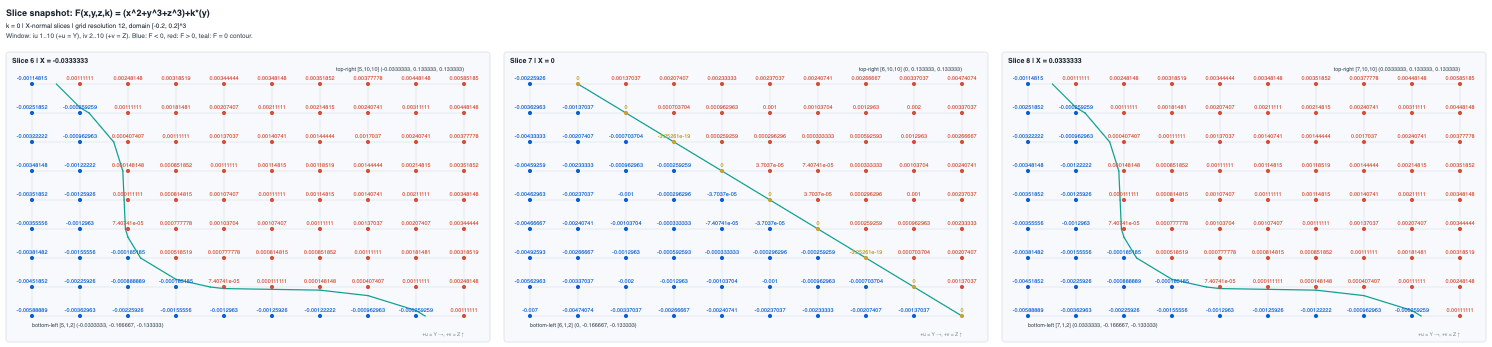
\includegraphics[width=\textwidth]{pictures/report/snap_D4a_k0.png}\\[4pt]
    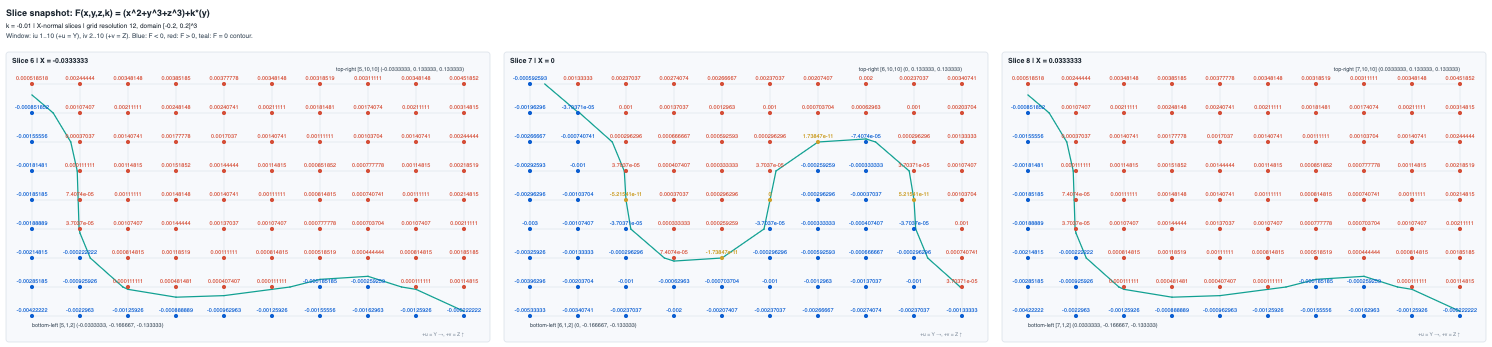
\includegraphics[width=\textwidth]{pictures/report/snap_D4a_kneg.png}\\[4pt]
    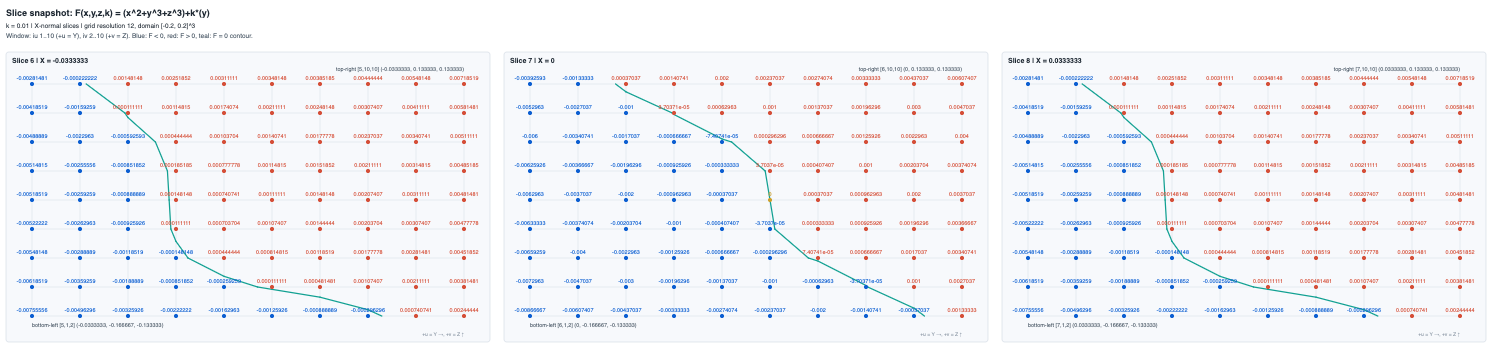
\includegraphics[width=\textwidth]{pictures/report/snap_D4a_kpos.png}
    \caption{Slice snapshots around the singular point of $x^2+y^3+z^3+kG$ with $G=y$:
    $k=0$ (top), $k<0$ (middle), $k>0$ (bottom); the values of $k$, the grid and
    the window are printed in each snapshot. Every node shows its value (blue
    negative, red positive, yellow zero); teal is the zero level $S_k$.}
    \label{fig:r-D4a-snap}
\end{figure}

\begin{table}[!h]
\centering
\footnotesize
\begin{adjustbox}{max width=\textwidth}
\begin{tabular}{l c l c c c c c c c}
\toprule
& & & & \multicolumn{2}{c}{$k<0$} & \multicolumn{2}{c}{$k>0$} & & \\
\cmidrule(lr){5-6}\cmidrule(lr){7-8}
$G$ & $m$ & essential part & predicted $\alpha$ & $\alpha$ & $C$ & $\alpha$ & $C$ & spread over $N$ & agrees \\
\midrule
$1$ & 0 & $1$ & $[\tfrac13,\tfrac12]$ & 0.332{\scriptsize$\pm$0.001} & 1.11 & 0.333{\scriptsize$\pm$0.000} & 1.00 & 0.002 & yes \\
$x$ & 1 & $0$ & $[\tfrac23,1]$ & 0.763{\scriptsize$\pm$0.069} & 1.22 & 0.763{\scriptsize$\pm$0.069} & 1.22 & 0.000 & yes \\
$y$ & 1 & $y$ & $[\tfrac12,\tfrac34]$ & 0.499{\scriptsize$\pm$0.000} & 1.03 & 0.500{\scriptsize$\pm$0.000} & 0.28 & 0.001 & yes \\
$z$ & 1 & $z$ & $[\tfrac12,\tfrac34]$ & 0.499{\scriptsize$\pm$0.000} & 1.03 & 0.500{\scriptsize$\pm$0.000} & 0.28 & 0.001 & yes \\
$x+y$ & 1 & $y$ & $[\tfrac12,\tfrac34]$ & 0.503{\scriptsize$\pm$0.001} & 1.06 & 0.513{\scriptsize$\pm$0.005} & 0.31 & 0.001 & yes \\
$x+z$ & 1 & $z$ & $[\tfrac12,\tfrac34]$ & 0.502{\scriptsize$\pm$0.002} & 1.06 & 0.513{\scriptsize$\pm$0.006} & 0.31 & 0.001 & yes \\
$x+y+z$ & 1 & $y + z$ & $[\tfrac12,\tfrac34]$ & 0.501{\scriptsize$\pm$0.001} & 1.43 & 0.774{\scriptsize$\pm$0.002} & 0.83 & 0.000 & \textbf{no} \\
$2x-y+3z$ & 1 & $-y + 3z$ & $[\tfrac12,\tfrac34]$ & 0.501{\scriptsize$\pm$0.001} & 1.61 & 0.508{\scriptsize$\pm$0.003} & 0.78 & 0.001 & yes \\
$x^2$ & 2 & $0$ & $1$ & 1.001{\scriptsize$\pm$0.001} & 0.05 & 0.999{\scriptsize$\pm$0.000} & 0.04 & 0.000 & yes \\
$x^2+y^2-z^2$ & 2 & $0$ & $1$ & 1.002{\scriptsize$\pm$0.001} & 0.82 & 1.002{\scriptsize$\pm$0.001} & 0.82 & 0.000 & yes \\
$xy$ & 2 & $0$ & $1$ & 0.900{\scriptsize$\pm$0.097} & 0.04 & 0.900{\scriptsize$\pm$0.097} & 0.04 & 0.101 & yes \\
$x^3$ & 3 & $0$ & $1$ & 1.000{\scriptsize$\pm$0.000} & 0.00 & 1.000{\scriptsize$\pm$0.000} & 0.00 & 0.000 & yes \\
$x^2y+y^2z+z^2x$ & 3 & $0$ & $1$ & 0.169{\scriptsize$\pm$0.152} & 0.00 & 0.169{\scriptsize$\pm$0.151} & 0.00 & 0.831 & \textbf{no} \\
$F$ & -- & $0$ & $1$ & $S_k=S_0$ & -- & $S_k=S_0$ & -- & -- & yes \\
\bottomrule
\end{tabular}
\end{adjustbox}
\caption[Rates for $x^2+y^3+z^3$]{All perturbations of $F=x^2+y^3+z^3$: convergence rates (resolution $128$). Columns are explained in Section~\ref{sec:r-read}.}
\label{tab:r-D4a-rates}
\end{table}
\begin{table}[!h]
\centering
\footnotesize
\begin{adjustbox}{max width=\textwidth}
\begin{tabular}{l l c l l c}
\toprule
$G$ & $P$ for $k\neq0$ & corank at $P$ & singular points, $k<0$ & singular points, $k>0$ & MC error \\
\midrule
$1$ & leaves $S_k$ & -- & none & none & 0.0014 \\
$x$ & regular & -- & none & none & 0.0226 \\
$y$ & regular & -- & none & none & 0.0021 \\
$z$ & regular & -- & none & none & 0.0021 \\
$x+y$ & regular & -- & none & none & 0.0024 \\
$x+z$ & regular & -- & none & none & 0.0023 \\
$x+y+z$ & regular & -- & none & none & 0.0062 \\
$2x-y+3z$ & regular & -- & none & none & 0.0020 \\
$x^2$ & singular & 2 & only $P$ & only $P$ & 0.0015 \\
$x^2+y^2-z^2$ & singular & 0 ($A_1$) & $P$ + 1$\times$$A_1$, $\gamma=1.00$ & $P$ + 1$\times$$A_1$, $\gamma=1.00$ & 0.0048 \\
$xy$ & singular & 1 & $P$; 1 more for some $k$ & $P$; 1 more for some $k$ & 0.0016 \\
$x^3$ & singular & 2 & only $P$ & only $P$ & 0.0015 \\
$x^2y+y^2z+z^2x$ & singular & 2 & only $P$ & only $P$ & 0.0015 \\
$F$ & singular & 2 & only $P$ & only $P$ & 0.0015 \\
\bottomrule
\end{tabular}
\end{adjustbox}
\caption[Singular points for $x^2+y^3+z^3$]{All perturbations of $F=x^2+y^3+z^3$: the point $P$, the singular points of $S_k$ and the accuracy of Marching Cubes. Columns are explained in Section~\ref{sec:r-read}.}
\label{tab:r-D4a-points}
\end{table}
\paragraph{Constant ($G=1$).} $0.332$ and $0.333$, the lower end $\tfrac13$, with
$C=1.11$ and $1.00$: in the $y,z$ directions the constant acts as on a cubic cone.

\paragraph{Linear $G$.} The essential $y$, $z$, $x+y$, $x+z$ and $2x-y+3z$ all give
$\alpha\approx0.50$ on both sides, but the constant is about four times larger for
$k<0$ ($1.03$) than for $k>0$ ($0.28$): for $k<0$ the cubic $y^3+ky$ gets two new
real zeros $\pm\sqrt{|k|}$ and the surface gets new sheets, for $k>0$ it only bends
(Figure~\ref{fig:r-D4a-snap}). $x+y+z$ has the essential part $y+z$ and gives
$0.774$ for $k>0$, slightly above $\tfrac34$, because its inessential part $x$ adds a
shift (``no'', as for the cusps).
The inessential $G=x$ gives $0.763$. Completing the square,
$(x+\tfrac k2)^2+y^3+z^3=\tfrac{k^2}{4}$: the surface is shifted by $k/2$ and receives
the constant $k^2/4$. On this surface a constant $c$ moves the surface by about
$|c|^{1/3}$ (the rate $\tfrac13$ of $G=1$), so the constant $k^2/4$ moves it by about
$(k^2/4)^{1/3}$, which is proportional to $|k|^{2/3}$. The measured $0.763$ lies
between this $\tfrac23$ and the rate $1$ of the shift, since both are visible in the
measured range of $k$. As for the horn cusp, this second-order effect is a thin
part of the surface that Marching Cubes misses: the extraction error is $0.0226$ in
Table~\ref{tab:r-D4a-points}, ten times that of the other linear perturbations.

\paragraph{Order two and three.} The origin stays singular. $x^2+y^2-z^2$ makes it
an ordinary double point. For $xy$ and $x^2y+y^2z+z^2x$ the deformation is so small
(of order $|k|\cdot10^{-4}$) that the measured distance reaches the resolution of the
measurement; the fitted $0.90$ and $0.17$ (``no'') describe the measurement, not
the surface (Section~\ref{sec:r-deviations}).

\paragraph{Singular points.} $x^2+y^2-z^2$ creates one more ordinary double point
that moves linearly ($\gamma=1$), as the conservation of the Milnor number allows
($4=1+1+2$, the last two complex). For $xy$ a second point is reported for some $k$
only, a resolution limit of the search.
\clearpage

\subsection{The $D_4$ point with three lines: $x^2+y^3-3yz^2$}
\label{sec:r-D4b}

The same type as $x^2+y^3+z^3$, but the cubic $y^3-3yz^2=y(y-\sqrt3z)(y+\sqrt3z)$
has \emph{three} real lines: on the plane $x=0$ the surface is three lines
through the origin at $60^\circ$ to each other (Figure~\ref{fig:r-D4b-exact}).
Basis $\{1,y,z,z^2\}$.

\begin{figure}[!h]
\centering
\begin{minipage}[c]{0.18\textwidth}\centering
      \centering
    \resizebox{\linewidth}{!}{\panel{exact_D4b_k0.png}} \\[2pt]
    {\footnotesize $k=0$}
\end{minipage}\hfill
\begin{minipage}[c]{0.72\textwidth}\centering
\begin{adjustbox}{max width=\textwidth}
\begin{tabular}{c c c}
$G$ & $k=-0.01$ & $k=+0.01$ \\
$1$ & \panel{exact_D4b_1_neg.png} & \panel{exact_D4b_1_pos.png} \\
$y$ & \panel{exact_D4b_y_neg.png} & \panel{exact_D4b_y_pos.png} \\
$z$ & \panel{exact_D4b_z_neg.png} & \panel{exact_D4b_z_pos.png} \\
\end{tabular}
\end{adjustbox}
\end{minipage}
\caption{Exact slices of $S_k$ on the plane $x=0$ (horizontal axis $y$, vertical
axis $z$, both from $-0.25$ to $0.25$), computed from the polynomial. Grey: the
singular surface $S_0$; blue: $S_k$; red: singular points of $S_k$ found by the
numerical stationary-point search; cross: the origin.}
\label{fig:r-D4b-exact}
\end{figure}

\begin{figure}[!h]
    \centering
    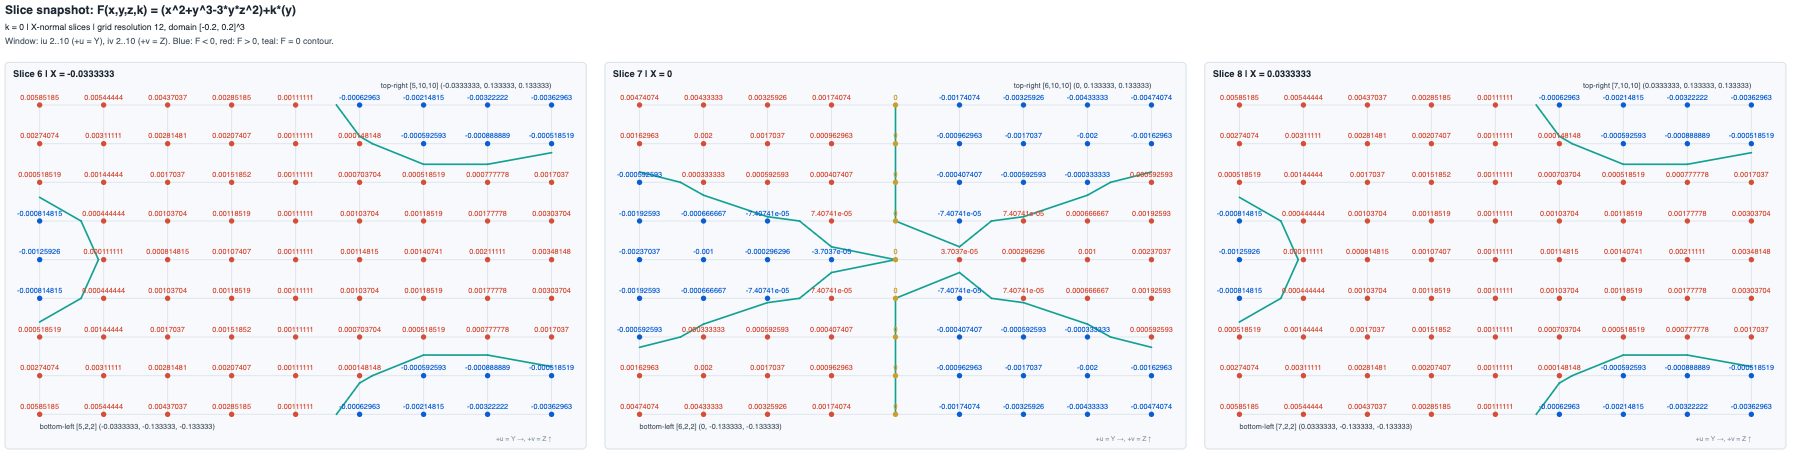
\includegraphics[width=\textwidth]{pictures/report/snap_D4b_k0.png}\\[4pt]
    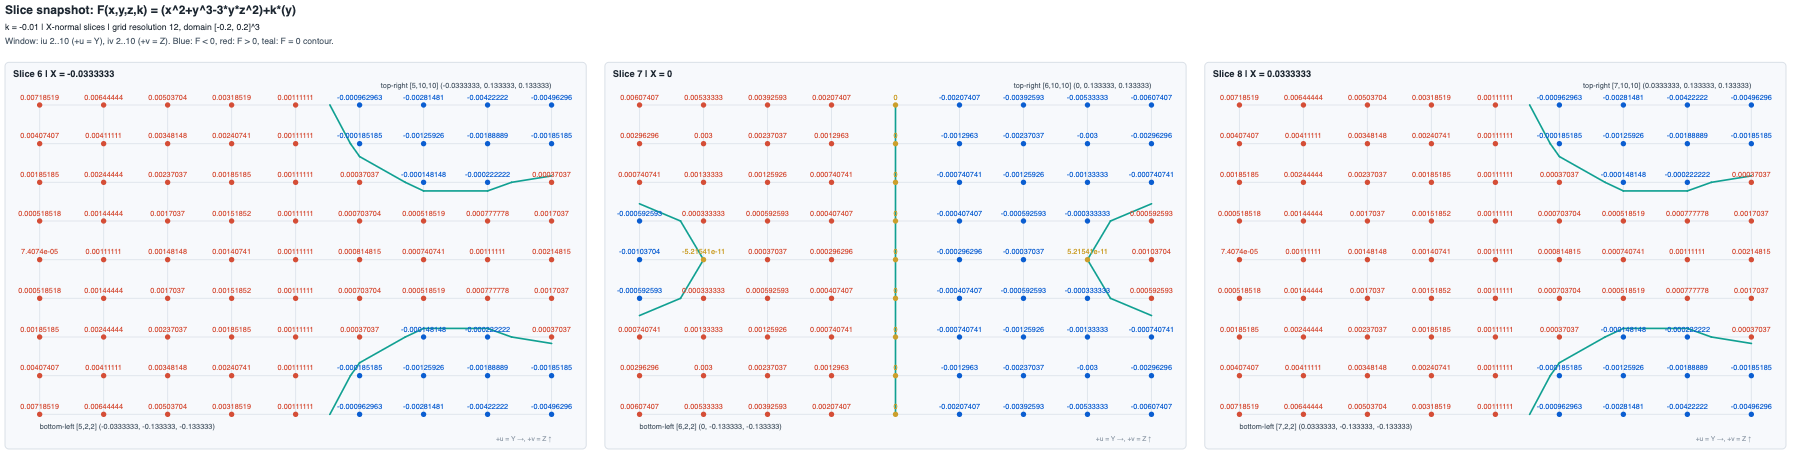
\includegraphics[width=\textwidth]{pictures/report/snap_D4b_kneg.png}\\[4pt]
    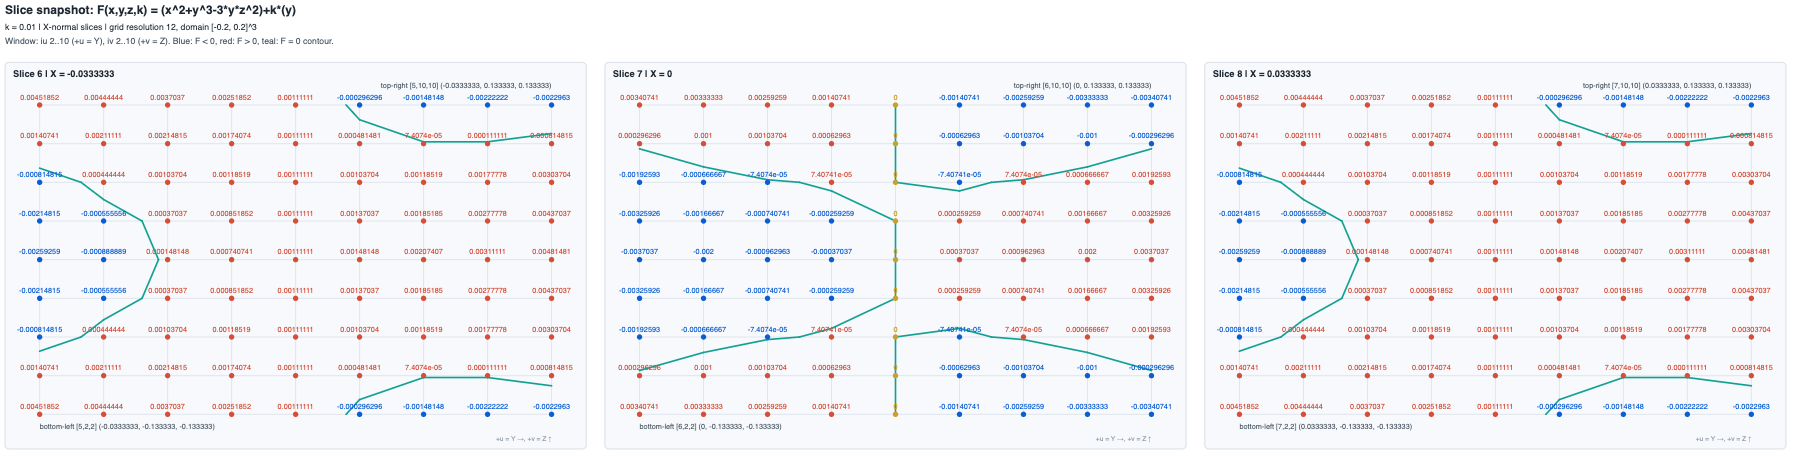
\includegraphics[width=\textwidth]{pictures/report/snap_D4b_kpos.png}
    \caption{Slice snapshots around the singular point of $x^2+y^3-3yz^2+kG$ with $G=y$:
    $k=0$ (top), $k<0$ (middle), $k>0$ (bottom); the values of $k$, the grid and
    the window are printed in each snapshot. Every node shows its value (blue
    negative, red positive, yellow zero); teal is the zero level $S_k$.}
    \label{fig:r-D4b-snap}
\end{figure}

\begin{table}[!h]
\centering
\footnotesize
\begin{adjustbox}{max width=\textwidth}
\begin{tabular}{l c l c c c c c c c}
\toprule
& & & & \multicolumn{2}{c}{$k<0$} & \multicolumn{2}{c}{$k>0$} & & \\
\cmidrule(lr){5-6}\cmidrule(lr){7-8}
$G$ & $m$ & essential part & predicted $\alpha$ & $\alpha$ & $C$ & $\alpha$ & $C$ & spread over $N$ & agrees \\
\midrule
$1$ & 0 & $1$ & $[\tfrac13,\tfrac12]$ & 0.332{\scriptsize$\pm$0.001} & 0.50 & 0.333{\scriptsize$\pm$0.001} & 1.00 & 0.001 & yes \\
$x$ & 1 & $0$ & $[\tfrac23,1]$ & 0.676{\scriptsize$\pm$0.011} & 0.34 & 0.676{\scriptsize$\pm$0.013} & 0.34 & 0.001 & yes \\
$y$ & 1 & $y$ & $[\tfrac12,\tfrac34]$ & 0.501{\scriptsize$\pm$0.004} & 0.53 & 0.504{\scriptsize$\pm$0.005} & 0.40 & 0.005 & yes \\
$z$ & 1 & $z$ & $[\tfrac12,\tfrac34]$ & 0.501{\scriptsize$\pm$0.005} & 0.53 & 0.501{\scriptsize$\pm$0.005} & 0.53 & 0.005 & yes \\
$x+y$ & 1 & $y$ & $[\tfrac12,\tfrac34]$ & 0.498{\scriptsize$\pm$0.004} & 0.51 & 0.493{\scriptsize$\pm$0.007} & 0.36 & 0.004 & yes \\
$x+z$ & 1 & $z$ & $[\tfrac12,\tfrac34]$ & 0.497{\scriptsize$\pm$0.005} & 0.51 & 0.497{\scriptsize$\pm$0.005} & 0.51 & 0.003 & yes \\
$x+y+z$ & 1 & $y + z$ & $[\tfrac12,\tfrac34]$ & 0.495{\scriptsize$\pm$0.002} & 0.54 & 0.499{\scriptsize$\pm$0.003} & 0.64 & 0.007 & yes \\
$2x-y+3z$ & 1 & $-y + 3z$ & $[\tfrac12,\tfrac34]$ & 0.499{\scriptsize$\pm$0.003} & 0.95 & 0.498{\scriptsize$\pm$0.005} & 0.80 & 0.004 & yes \\
$x^2$ & 2 & $0$ & $1$ & 1.002{\scriptsize$\pm$0.001} & 0.04 & 0.999{\scriptsize$\pm$0.001} & 0.04 & 0.001 & yes \\
$x^2+y^2-z^2$ & 2 & $0$ & $1$ & 0.877{\scriptsize$\pm$0.181} & 0.26 & 0.633{\scriptsize$\pm$0.232} & 0.05 & 0.430 & \textbf{no} \\
$xy$ & 2 & $0$ & $1$ & 0.267{\scriptsize$\pm$0.312} & 0.00 & 0.267{\scriptsize$\pm$0.312} & 0.00 & 0.191 & \textbf{no} \\
$x^3$ & 3 & $0$ & $1$ & 1.000{\scriptsize$\pm$0.000} & 0.00 & 1.000{\scriptsize$\pm$0.000} & 0.00 & 0.000 & yes \\
$x^2y+y^2z+z^2x$ & 3 & $0$ & $1$ & 0.936{\scriptsize$\pm$0.359} & 0.05 & 0.809{\scriptsize$\pm$0.327} & 0.02 & 0.127 & yes \\
$F$ & -- & $0$ & $1$ & $S_k=S_0$ & -- & $S_k=S_0$ & -- & -- & yes \\
\bottomrule
\end{tabular}
\end{adjustbox}
\caption[Rates for $x^2+y^3-3yz^2$]{All perturbations of $F=x^2+y^3-3yz^2$: convergence rates (resolution $128$). Columns are explained in Section~\ref{sec:r-read}.}
\label{tab:r-D4b-rates}
\end{table}
\begin{table}[!h]
\centering
\footnotesize
\begin{adjustbox}{max width=\textwidth}
\begin{tabular}{l l c l l c}
\toprule
$G$ & $P$ for $k\neq0$ & corank at $P$ & singular points, $k<0$ & singular points, $k>0$ & MC error \\
\midrule
$1$ & leaves $S_k$ & -- & none & none & 0.0013 \\
$x$ & regular & -- & none & none & 0.0101 \\
$y$ & regular & -- & none & 2$\times$$A_1$, $\gamma=0.50$ & 0.0028 \\
$z$ & regular & -- & none & none & 0.0017 \\
$x+y$ & regular & -- & none & none & 0.0063 \\
$x+z$ & regular & -- & none & none & 0.0022 \\
$x+y+z$ & regular & -- & none & none & 0.0021 \\
$2x-y+3z$ & regular & -- & none & none & 0.0021 \\
$x^2$ & singular & 2 & only $P$ & only $P$ & 0.0027 \\
$x^2+y^2-z^2$ & singular & 0 ($A_1$) & only $P$ & only $P$ & 0.0031 \\
$xy$ & singular & 1 & $P$; 1 more for some $k$ & $P$; 1 more for some $k$ & 0.0027 \\
$x^3$ & singular & 2 & only $P$ & only $P$ & 0.0027 \\
$x^2y+y^2z+z^2x$ & singular & 2 & only $P$ & only $P$ & 0.0027 \\
$F$ & singular & 2 & only $P$ & only $P$ & 0.0027 \\
\bottomrule
\end{tabular}
\end{adjustbox}
\caption[Singular points for $x^2+y^3-3yz^2$]{All perturbations of $F=x^2+y^3-3yz^2$: the point $P$, the singular points of $S_k$ and the accuracy of Marching Cubes. Columns are explained in Section~\ref{sec:r-read}.}
\label{tab:r-D4b-points}
\end{table}
\paragraph{Constant ($G=1$).} $0.332$ and $0.333$, as for the other $D_4$ surface;
the constant $C$ is $0.50$ for $k<0$ and $1.00$ for $k>0$.

\paragraph{Linear $G$.} All essential linear $G$ give $\alpha\approx0.50$ on
\emph{both} sides with similar constants. Unlike the one-line case, three real lines
leave no direction in which the perturbation can only bend the surface: some pair
of lines is always pulled apart on the scale $\sqrt{|k|}$. The inessential $x$ gives
$0.676$: as for $x^2+y^3+z^3$, a shift by $k/2$ plus the constant $k^2/4$, whose
effect is proportional to $|k|^{2/3}$; here the measured rate is close to $\tfrac23$
itself.

\paragraph{Order two and three.} $x^2$ and $x^3$ give $1.00$. For $xy$,
$x^2+y^2-z^2$ and $x^2y+y^2z+z^2x$ the deformation is again near the resolution of
the measurement, and the fitted values ($0.27$--$0.94$, two of them ``no'') are not
reliable (Section~\ref{sec:r-deviations}).

\paragraph{Singular points.} $G=y$ creates two ordinary double points for $k>0$.
The slice $x=0$ becomes $y(y^2-3z^2+k)=0$: the line $y=0$ and the hyperbola
$y^2-3z^2=-k$, which meet at $(0,0,\pm\sqrt{k/3})$. These are found by the
numerical stationary-point search for every $k>0$ and move with $\gamma=0.50$
(Figures~\ref{fig:r-D4b-exact} and~\ref{fig:r-D4b-snap}). For $k<0$ the hyperbola
opens the other way and does not meet the line.
\clearpage

\subsection{The Fermat cone $x^3+y^3+z^3$}
\label{sec:r-E6a}

A homogeneous cubic: every line through the origin and a point of the
surface lies on the surface, so the surface is a \emph{cone} over the real cubic
curve $x^3+y^3+z^3=0$. That curve is a single closed curve of the projective
plane, so the cone is one wavy sheet through the origin (Figure~\ref{fig:r-E6a-iso}).
All weights are $\tfrac13$, $\mu=\tau=8$, and the essential directions are
$1,x,y,z,xy,xz,yz,xyz$; $x^2,y^2,z^2$ and the pure cubes are inessential.
Because $F$ is homogeneous, a homogeneous $G$ of degree $m$ gives an
\emph{exactly} self-similar family: $S_k$ is a fixed surface scaled by
$|k|^{1/(3-m)}$.

\begin{figure}[!h]
    \centering
    \begin{subfigure}{0.3\textwidth}\centering
        \thesisimage{pictures/ch3/cone_Fplus.png}{0.8\textwidth}{4cm}{$F_+$, $k=0$}
        \caption{$k=0$}\end{subfigure}
    \caption{$x^3+y^3+z^3$ extracted by Marching Cubes, coloured by $\|\nabla F\|$
    (blue: small gradient). The singular point is the dark spot in the middle.}
    \label{fig:r-E6a-iso}
\end{figure}

\begin{figure}[!h]
    \centering
    \begin{subfigure}{0.31\textwidth}\centering
        \thesisimage{pictures/ch4/G1_kneg.png}{0.85\textwidth}{4cm}{$F_++k$, $k<0$}
        \caption{$k<0$}\end{subfigure}\hfill
    \begin{subfigure}{0.31\textwidth}\centering
        \thesisimage{pictures/ch4/G1_k0.png}{0.85\textwidth}{4cm}{$F_+$, $k=0$}
        \caption{$k=0$}\end{subfigure}\hfill
    \begin{subfigure}{0.31\textwidth}\centering
        \thesisimage{pictures/ch4/G1_kpos.png}{0.85\textwidth}{4cm}{$F_++k$, $k>0$}
        \caption{$k>0$}\end{subfigure}
    \caption{$x^3+y^3+z^3+k$: the apex of the cone is replaced by a smooth cap
    (isosurfaces from the viewer, $|k|=0.005$).}
    \label{fig:r-E6a-G1}
\end{figure}

\begin{figure}[!h]
\centering
\begin{minipage}[c]{0.18\textwidth}\centering
      \centering
    \resizebox{\linewidth}{!}{\panel{exact_E6a_k0.png}} \\[2pt]
    {\footnotesize $k=0$}
\end{minipage}\hfill
\begin{minipage}[c]{0.72\textwidth}\centering
\begin{adjustbox}{max width=\textwidth}
\begin{tabular}{c c c}
$G$ & $k=-0.01$ & $k=+0.01$ \\
$1$ & \panel{exact_E6a_1_neg.png} & \panel{exact_E6a_1_pos.png} \\
$x+y$ & \panel{exact_E6a_xpy_neg.png} & \panel{exact_E6a_xpy_pos.png} \\
$x^2+y^2-z^2$ & \panel{exact_E6a_x2py2mz2_neg.png} & \panel{exact_E6a_x2py2mz2_pos.png} \\
\end{tabular}
\end{adjustbox}
\end{minipage}
\caption{Exact slices of $S_k$ on the plane $z=0$ (horizontal axis $x$, vertical
axis $y$, both from $-0.25$ to $0.25$), computed from the polynomial. Grey: the
singular surface $S_0$; blue: $S_k$; red: singular points of $S_k$ found by the
numerical stationary-point search; cross: the origin.}
\label{fig:r-E6a-exact}
\end{figure}

\begin{figure}[!h]
    \centering
    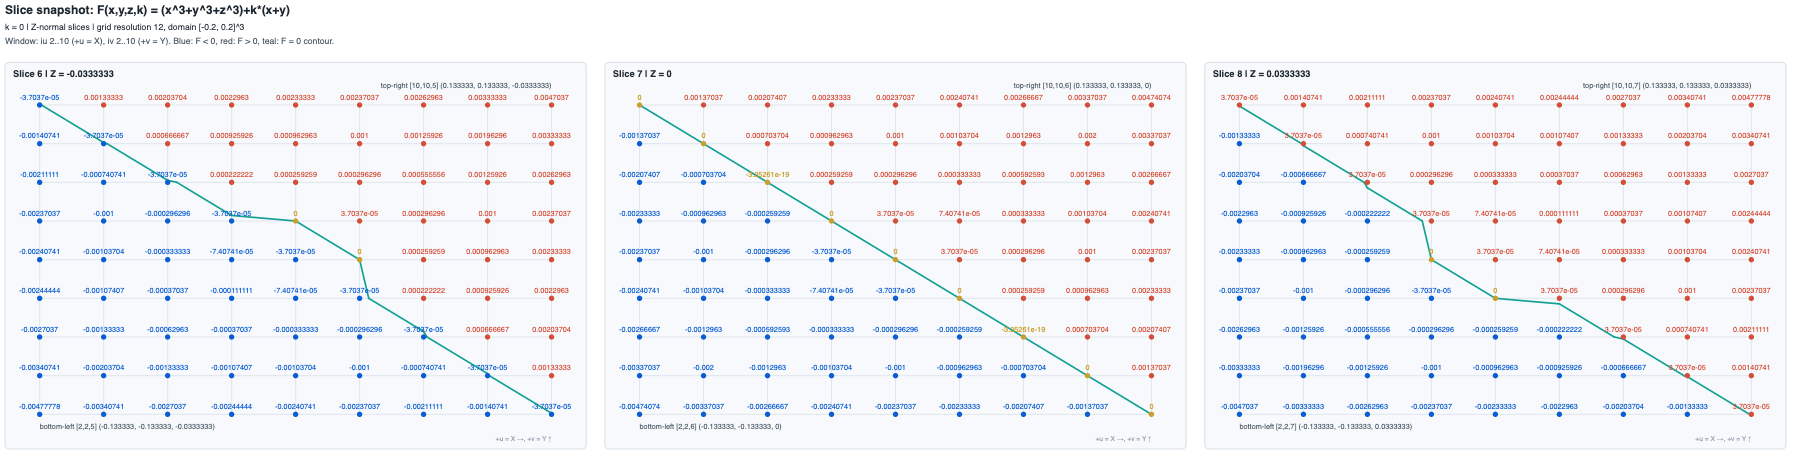
\includegraphics[width=\textwidth]{pictures/report/snap_E6a_k0.png}\\[4pt]
    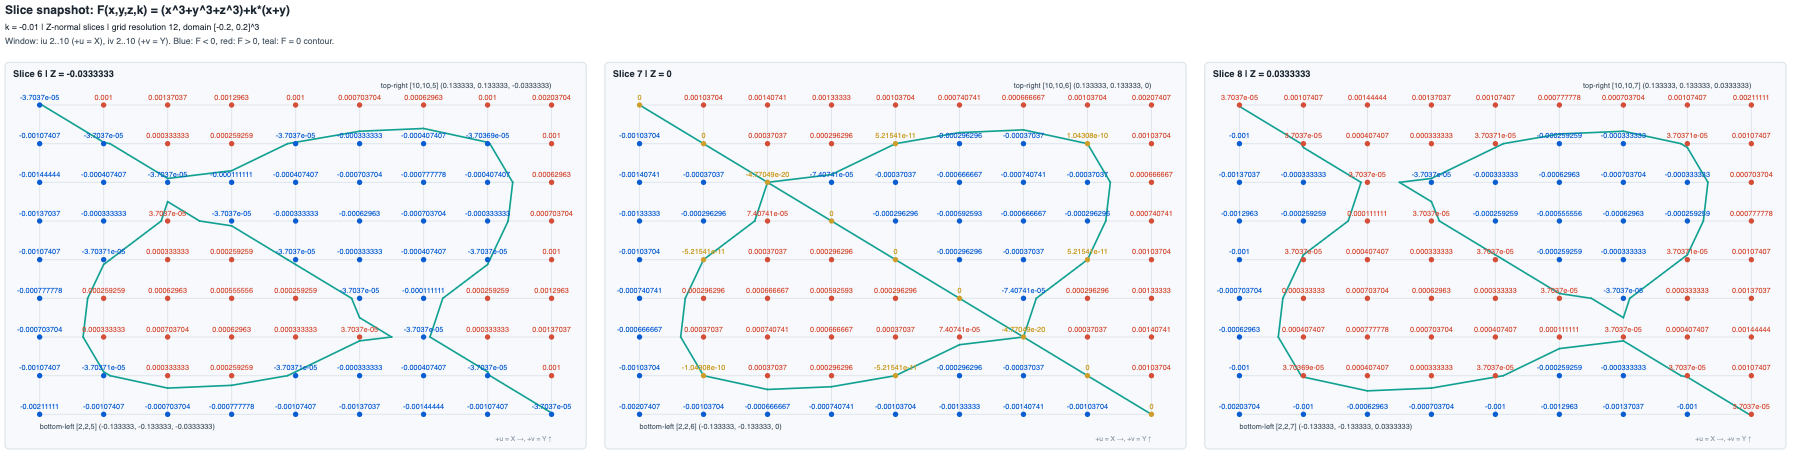
\includegraphics[width=\textwidth]{pictures/report/snap_E6a_kneg.png}\\[4pt]
    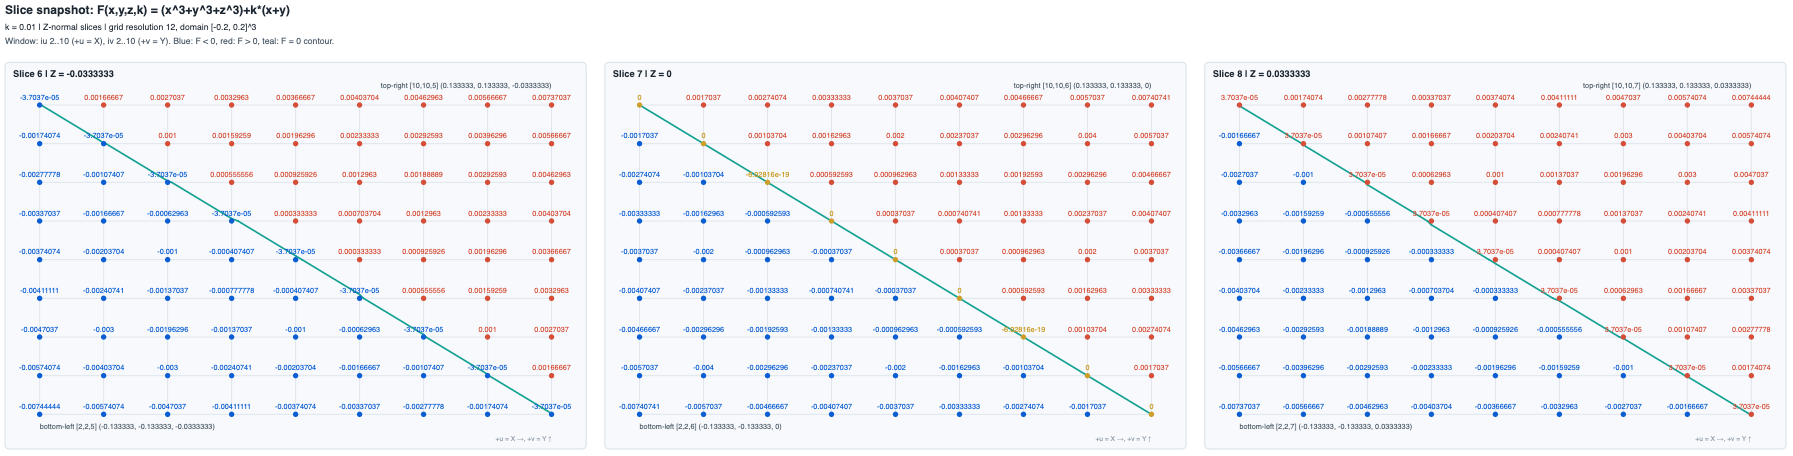
\includegraphics[width=\textwidth]{pictures/report/snap_E6a_kpos.png}
    \caption{Slice snapshots around the singular point of $x^3+y^3+z^3+kG$ with $G=x+y$:
    $k=0$ (top), $k<0$ (middle), $k>0$ (bottom); the values of $k$, the grid and
    the window are printed in each snapshot. Every node shows its value (blue
    negative, red positive, yellow zero); teal is the zero level $S_k$.}
    \label{fig:r-E6a-snap}
\end{figure}

\begin{table}[!h]
\centering
\footnotesize
\begin{adjustbox}{max width=\textwidth}
\begin{tabular}{l c l c c c c c c c}
\toprule
& & & & \multicolumn{2}{c}{$k<0$} & \multicolumn{2}{c}{$k>0$} & & \\
\cmidrule(lr){5-6}\cmidrule(lr){7-8}
$G$ & $m$ & essential part & predicted $\alpha$ & $\alpha$ & $C$ & $\alpha$ & $C$ & spread over $N$ & agrees \\
\midrule
$1$ & 0 & $1$ & $\tfrac13$ & 0.333{\scriptsize$\pm$0.007} & 1.16 & 0.333{\scriptsize$\pm$0.007} & 1.16 & 0.002 & yes \\
$x$ & 1 & $x$ & $\tfrac12$ & 0.501{\scriptsize$\pm$0.001} & 1.03 & 0.500{\scriptsize$\pm$0.000} & 0.29 & 0.001 & yes \\
$y$ & 1 & $y$ & $\tfrac12$ & 0.501{\scriptsize$\pm$0.001} & 1.03 & 0.500{\scriptsize$\pm$0.000} & 0.29 & 0.001 & yes \\
$z$ & 1 & $z$ & $\tfrac12$ & 0.501{\scriptsize$\pm$0.001} & 1.03 & 0.500{\scriptsize$\pm$0.000} & 0.29 & 0.001 & yes \\
$x+y$ & 1 & $x + y$ & $\tfrac12$ & 0.500{\scriptsize$\pm$0.000} & 1.38 & 0.500{\scriptsize$\pm$0.000} & 0.37 & 0.000 & yes \\
$x+z$ & 1 & $x + z$ & $\tfrac12$ & 0.500{\scriptsize$\pm$0.000} & 1.38 & 0.500{\scriptsize$\pm$0.000} & 0.37 & 0.000 & yes \\
$x+y+z$ & 1 & $x + y + z$ & $\tfrac12$ & 0.500{\scriptsize$\pm$0.000} & 1.69 & 0.500{\scriptsize$\pm$0.000} & 0.11 & 0.006 & yes \\
$2x-y+3z$ & 1 & $2x - y + 3z$ & $\tfrac12$ & 0.500{\scriptsize$\pm$0.000} & 2.00 & 0.500{\scriptsize$\pm$0.000} & 0.80 & 0.002 & yes \\
$x^2$ & 2 & $0$ & $1$ & 1.034{\scriptsize$\pm$0.035} & 1.11 & 1.006{\scriptsize$\pm$0.006} & 0.94 & 0.005 & yes \\
$x^2+y^2-z^2$ & 2 & $0$ & $1$ & 1.002{\scriptsize$\pm$0.003} & 1.12 & 1.002{\scriptsize$\pm$0.003} & 1.12 & 0.002 & yes \\
$xy$ & 2 & $xy$ & $1$ & 1.030{\scriptsize$\pm$0.032} & 0.74 & 0.996{\scriptsize$\pm$0.007} & 0.61 & 0.001 & yes \\
$x^3$ & 3 & $0$ & $1$ & 1.001{\scriptsize$\pm$0.000} & 0.05 & 0.999{\scriptsize$\pm$0.000} & 0.04 & 0.000 & yes \\
$x^2y+y^2z+z^2x$ & 3 & $0$ & $1$ & 1.000{\scriptsize$\pm$0.000} & 0.05 & 1.000{\scriptsize$\pm$0.000} & 0.05 & 0.000 & yes \\
$x+y+1.5874z$ & 1 & $x + y + 1.587z$ & $\tfrac12$ & 0.500{\scriptsize$\pm$0.000} & 1.84 & 0.500{\scriptsize$\pm$0.000} & 0.19 & 0.001 & yes \\
$F$ & -- & $0$ & $1$ & $S_k=S_0$ & -- & $S_k=S_0$ & -- & -- & yes \\
\bottomrule
\end{tabular}
\end{adjustbox}
\caption[Rates for $x^3+y^3+z^3$]{All perturbations of $F=x^3+y^3+z^3$: convergence rates (resolution $128$). Columns are explained in Section~\ref{sec:r-read}.}
\label{tab:r-E6a-rates}
\end{table}
\begin{table}[!h]
\centering
\footnotesize
\begin{adjustbox}{max width=\textwidth}
\begin{tabular}{l l c l l c}
\toprule
$G$ & $P$ for $k\neq0$ & corank at $P$ & singular points, $k<0$ & singular points, $k>0$ & MC error \\
\midrule
$1$ & leaves $S_k$ & -- & none & none & 0.0005 \\
$x$ & regular & -- & none & none & 0.0029 \\
$y$ & regular & -- & none & none & 0.0029 \\
$z$ & regular & -- & none & none & 0.0029 \\
$x+y$ & regular & -- & 2$\times$$A_2$, $\gamma=0.50$ & none & 0.0026 \\
$x+z$ & regular & -- & 2$\times$$A_2$, $\gamma=0.50$ & none & 0.0026 \\
$x+y+z$ & regular & -- & none & none & 0.0027 \\
$2x-y+3z$ & regular & -- & none & none & 0.0017 \\
$x^2$ & singular & 2 & only $P$ & only $P$ & 0.0036 \\
$x^2+y^2-z^2$ & singular & 0 ($A_1$) & $P$ + 2$\times$$A_1$, $\gamma=1.00$ & $P$ + 2$\times$$A_1$, $\gamma=1.00$ & 0.0059 \\
$xy$ & singular & 1 & only $P$ & only $P$ & 0.0064 \\
$x^3$ & singular & 3 & only $P$ & only $P$ & 0.0018 \\
$x^2y+y^2z+z^2x$ & singular & 3 & only $P$ & only $P$ & 0.0017 \\
$x+y+1.5874z$ & regular & -- & 2$\times$$A_1$, $\gamma=0.50$ & none & 0.0026 \\
$F$ & singular & 3 & only $P$ & only $P$ & 0.0019 \\
\bottomrule
\end{tabular}
\end{adjustbox}
\caption[Singular points for $x^3+y^3+z^3$]{All perturbations of $F=x^3+y^3+z^3$: the point $P$, the singular points of $S_k$ and the accuracy of Marching Cubes. Columns are explained in Section~\ref{sec:r-read}.}
\label{tab:r-E6a-points}
\end{table}
\paragraph{Constant ($G=1$).} The apex is replaced by a smooth cap
(Figure~\ref{fig:r-E6a-G1}). The distance from the origin to $S_k$ is exactly
$|k|^{1/3}$; the Hausdorff distance is $1.163\,|k|^{1/3}$, because the cap is
farthest from the cone in the direction $(1,1,1)$. The measured rate is $0.333$.

\paragraph{Linear $G$.} Every linear $G$ is essential and gives $0.500$ on both
sides and at every resolution (the spread over $N$ is at most $0.006$). This is the
self-similarity at work: only the constant depends on the direction of $G$. It is
larger for $k<0$ ($1.03$ for $x$) than for $k>0$ ($0.29$): for $k<0$ the cone opens
with new real structure, for $k>0$ it only smooths.

\paragraph{Order two and three.} Every $G$ of order two or three gives $1.00$. $x^2$
is inessential (a translation by $k/3$) and the origin stays singular with corank
$2$. $x^2+y^2-z^2$ makes the origin an ordinary double point. $xy$ is essential and
keeps the origin singular with corank $1$. $x^3$ stretches the cone along $x$
($x^3+kx^3=(\sqrt[3]{1+k}\,x)^3$) and $x^2y+y^2z+z^2x$ changes its shape; both keep the
type of the singular point and have tiny constants ($0.05$).

\paragraph{Singular points.} For a diagonal cone $F=a_1x^3+a_2y^3+a_3z^3$ and a
linear $G=c_1x+c_2y+c_3z$, the stationary points satisfy $3a_ix_i^2=-kc_i$, and at
each of them $H_k=\tfrac{2k}{3}G$. Hence a stationary point lies on the surface
exactly when $G=0$ there, which happens when
\[
\pm c_1|c_1/a_1|^{1/2}\pm c_2|c_2/a_2|^{1/2}\pm c_3|c_3/a_3|^{1/2}=0
\]
for some choice of signs (terms with $c_i=0$ left out). Then $S_k$ has singular points
at the distance $\sqrt{|k|/3}\,(\sum|c_i/a_i|)^{1/2}$ from $P$, i.e.\ moving with
$\gamma=\tfrac12$. For $x^3+y^3+z^3$ and $k<0$ the stationary points are real exactly
when all $c_i\ge0$. Hence:
\begin{itemize}
    \item $x$, $y$, $z$, $x+y+z$, $2x-y+3z$: no singular points;
    \item $x+y$ and $x+z$: $1-1=0$, two cusps ($A_2$) at $(\pm s,\mp s,0)$,
          $s=\sqrt{|k|/3}$, for $k<0$ only, moving with $\gamma=0.500$
          (Figures~\ref{fig:r-E6a-exact} and~\ref{fig:r-E6a-snap}; in the slice
          $z=0$ the surface is the line $x=-y$ and an ellipse, and the cusps are
          where they meet);
    \item the balanced $x+y+1.5874z$: $1+1-(1.5874)^{3/2}=0$, two ordinary double
          points, $\gamma=0.500$ (Section~\ref{sec:r-sweep}).
\end{itemize}
Among the perturbations of order two, $x^2+y^2-z^2$ adds two ordinary double points
that move linearly ($\gamma=1$): together with $P$, three of the eight units of the
Milnor number become real singular points.
\clearpage

\subsection{The Fermat cone $x^3+y^3-z^3$}
\label{sec:r-E6b}

This is the mirror image of $x^3+y^3+z^3$ under $z\mapsto-z$. Every result
for it is a result for $x^3+y^3+z^3$ with $z$ replaced by $-z$ in $G$.

\begin{figure}[!h]
    \centering
    \thesisimage{pictures/ch3/cone_Fminus.png}{0.25\textwidth}{4cm}{$F_-$, $k=0$}
    \caption{$x^3+y^3-z^3$ extracted by Marching Cubes, coloured by $\|\nabla F\|$.}
    \label{fig:r-E6b-iso}
\end{figure}

\begin{figure}[!h]
\centering
\begin{minipage}[c]{0.18\textwidth}\centering
      \centering
    \resizebox{\linewidth}{!}{\panel{exact_E6b_k0.png}} \\[2pt]
    {\footnotesize $k=0$}
\end{minipage}\hfill
\begin{minipage}[c]{0.72\textwidth}\centering
\begin{adjustbox}{max width=\textwidth}
\begin{tabular}{c c c}
$G$ & $k=-0.01$ & $k=+0.01$ \\
$1$ & \panel{exact_E6b_1_neg.png} & \panel{exact_E6b_1_pos.png} \\
$x+y$ & \panel{exact_E6b_xpy_neg.png} & \panel{exact_E6b_xpy_pos.png} \\
$x^2+y^2-z^2$ & \panel{exact_E6b_x2py2mz2_neg.png} & \panel{exact_E6b_x2py2mz2_pos.png} \\
\end{tabular}
\end{adjustbox}
\end{minipage}
\caption{Exact slices of $S_k$ on the plane $z=0$ (horizontal axis $x$, vertical
axis $y$, both from $-0.25$ to $0.25$), computed from the polynomial. Grey: the
singular surface $S_0$; blue: $S_k$; red: singular points of $S_k$ found by the
numerical stationary-point search; cross: the origin.}
\label{fig:r-E6b-exact}
\end{figure}

\begin{figure}[!h]
    \centering
    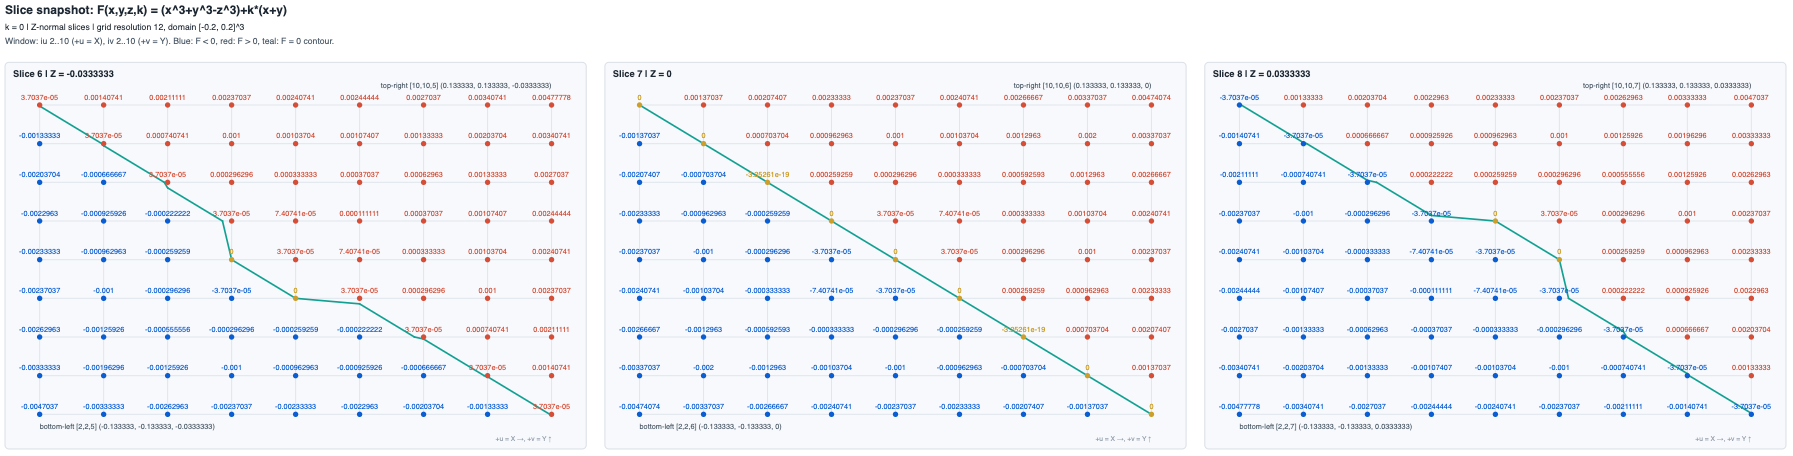
\includegraphics[width=\textwidth]{pictures/report/snap_E6b_k0.png}\\[4pt]
    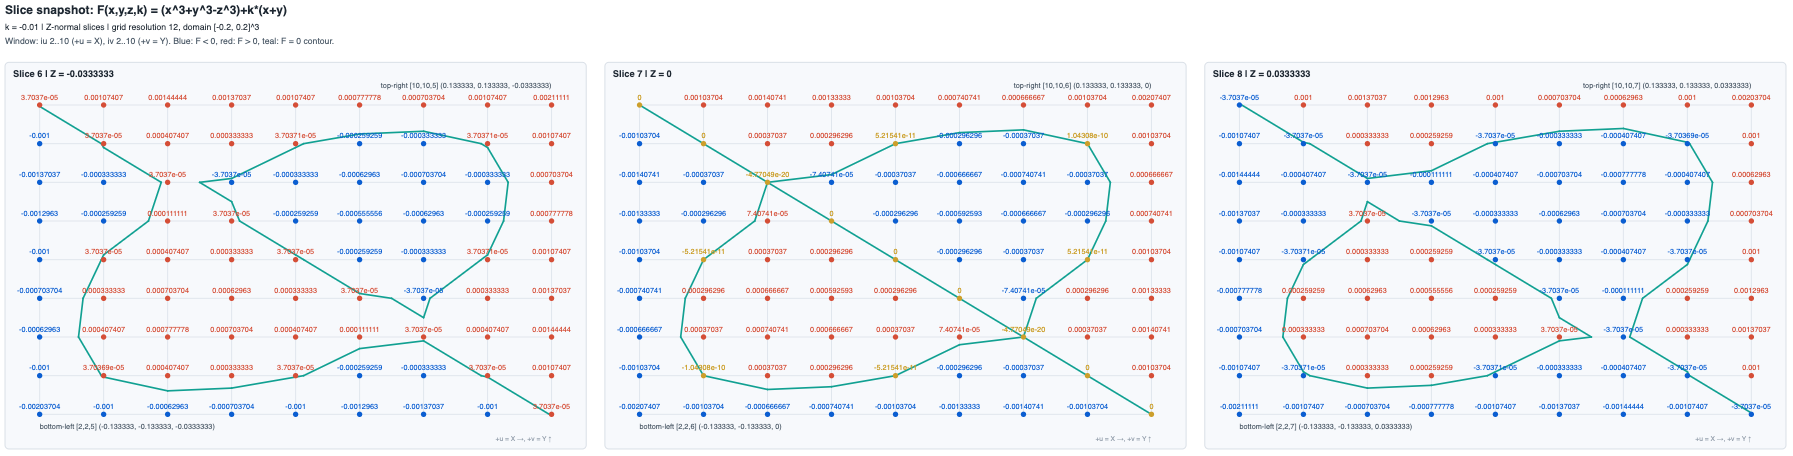
\includegraphics[width=\textwidth]{pictures/report/snap_E6b_kneg.png}\\[4pt]
    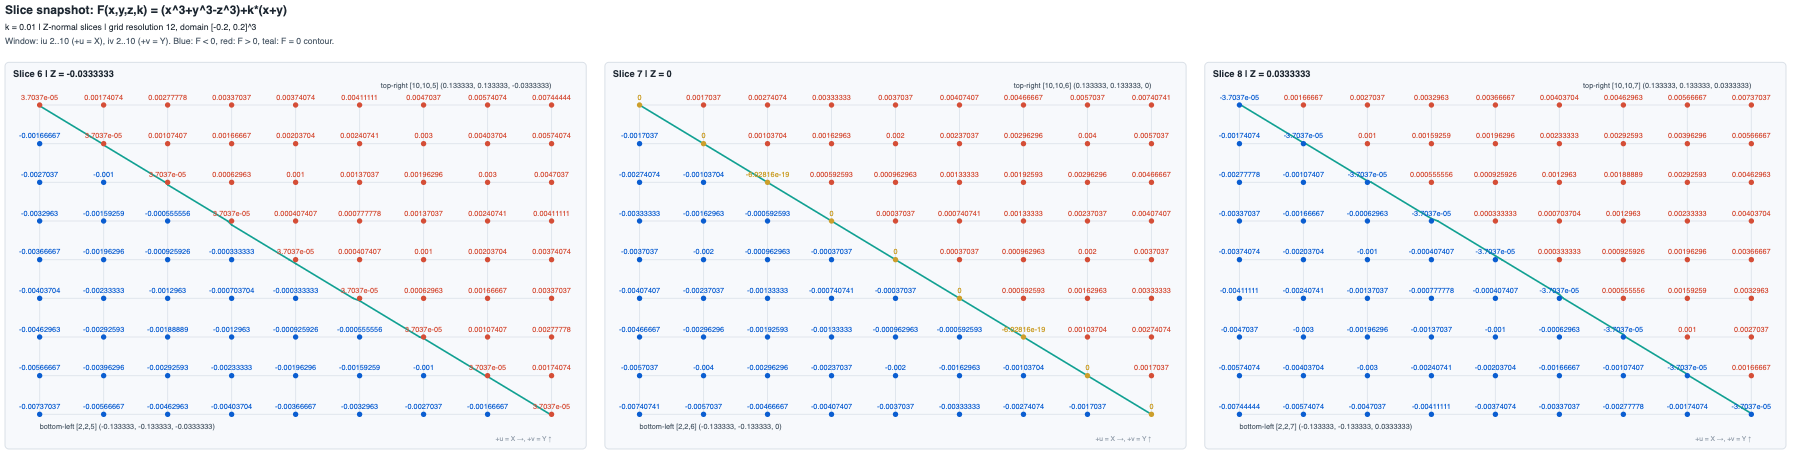
\includegraphics[width=\textwidth]{pictures/report/snap_E6b_kpos.png}
    \caption{Slice snapshots around the singular point of $x^3+y^3-z^3+kG$ with $G=x+y$:
    $k=0$ (top), $k<0$ (middle), $k>0$ (bottom); the values of $k$, the grid and
    the window are printed in each snapshot. Every node shows its value (blue
    negative, red positive, yellow zero); teal is the zero level $S_k$.}
    \label{fig:r-E6b-snap}
\end{figure}

\begin{table}[!h]
\centering
\footnotesize
\begin{adjustbox}{max width=\textwidth}
\begin{tabular}{l c l c c c c c c c}
\toprule
& & & & \multicolumn{2}{c}{$k<0$} & \multicolumn{2}{c}{$k>0$} & & \\
\cmidrule(lr){5-6}\cmidrule(lr){7-8}
$G$ & $m$ & essential part & predicted $\alpha$ & $\alpha$ & $C$ & $\alpha$ & $C$ & spread over $N$ & agrees \\
\midrule
$1$ & 0 & $1$ & $\tfrac13$ & 0.333{\scriptsize$\pm$0.007} & 1.16 & 0.333{\scriptsize$\pm$0.007} & 1.16 & 0.002 & yes \\
$x$ & 1 & $x$ & $\tfrac12$ & 0.501{\scriptsize$\pm$0.001} & 1.03 & 0.500{\scriptsize$\pm$0.000} & 0.29 & 0.001 & yes \\
$y$ & 1 & $y$ & $\tfrac12$ & 0.501{\scriptsize$\pm$0.001} & 1.03 & 0.500{\scriptsize$\pm$0.000} & 0.29 & 0.001 & yes \\
$z$ & 1 & $z$ & $\tfrac12$ & 0.500{\scriptsize$\pm$0.000} & 0.29 & 0.501{\scriptsize$\pm$0.001} & 1.03 & 0.001 & yes \\
$x+y$ & 1 & $x + y$ & $\tfrac12$ & 0.500{\scriptsize$\pm$0.000} & 1.38 & 0.500{\scriptsize$\pm$0.000} & 0.37 & 0.000 & yes \\
$x+z$ & 1 & $x + z$ & $\tfrac12$ & 0.500{\scriptsize$\pm$0.000} & 0.77 & 0.500{\scriptsize$\pm$0.000} & 0.77 & 0.000 & yes \\
$x+y+z$ & 1 & $x + y + z$ & $\tfrac12$ & 0.500{\scriptsize$\pm$0.000} & 1.11 & 0.501{\scriptsize$\pm$0.001} & 0.72 & 0.000 & yes \\
$2x-y+3z$ & 1 & $2x - y + 3z$ & $\tfrac12$ & 0.500{\scriptsize$\pm$0.001} & 1.01 & 0.500{\scriptsize$\pm$0.000} & 1.61 & 0.001 & yes \\
$x^2$ & 2 & $0$ & $1$ & 1.034{\scriptsize$\pm$0.035} & 1.11 & 1.006{\scriptsize$\pm$0.006} & 0.94 & 0.005 & yes \\
$x^2+y^2-z^2$ & 2 & $0$ & $1$ & 1.002{\scriptsize$\pm$0.003} & 1.12 & 1.002{\scriptsize$\pm$0.003} & 1.12 & 0.002 & yes \\
$xy$ & 2 & $xy$ & $1$ & 1.030{\scriptsize$\pm$0.032} & 0.74 & 0.996{\scriptsize$\pm$0.007} & 0.61 & 0.001 & yes \\
$x^3$ & 3 & $0$ & $1$ & 1.001{\scriptsize$\pm$0.000} & 0.05 & 0.999{\scriptsize$\pm$0.000} & 0.04 & 0.000 & yes \\
$x^2y+y^2z+z^2x$ & 3 & $0$ & $1$ & 1.001{\scriptsize$\pm$0.001} & 0.09 & 1.000{\scriptsize$\pm$0.000} & 0.09 & 0.000 & yes \\
$x+y-1.5874z$ & 1 & $x + y - 1.587z$ & $\tfrac12$ & 0.501{\scriptsize$\pm$0.001} & 1.85 & 0.500{\scriptsize$\pm$0.000} & 0.19 & 0.000 & yes \\
$F$ & -- & $0$ & $1$ & $S_k=S_0$ & -- & $S_k=S_0$ & -- & -- & yes \\
\bottomrule
\end{tabular}
\end{adjustbox}
\caption[Rates for $x^3+y^3-z^3$]{All perturbations of $F=x^3+y^3-z^3$: convergence rates (resolution $128$). Columns are explained in Section~\ref{sec:r-read}.}
\label{tab:r-E6b-rates}
\end{table}
\begin{table}[!h]
\centering
\footnotesize
\begin{adjustbox}{max width=\textwidth}
\begin{tabular}{l l c l l c}
\toprule
$G$ & $P$ for $k\neq0$ & corank at $P$ & singular points, $k<0$ & singular points, $k>0$ & MC error \\
\midrule
$1$ & leaves $S_k$ & -- & none & none & 0.0005 \\
$x$ & regular & -- & none & none & 0.0029 \\
$y$ & regular & -- & none & none & 0.0029 \\
$z$ & regular & -- & none & none & 0.0029 \\
$x+y$ & regular & -- & 2$\times$$A_2$, $\gamma=0.50$ & none & 0.0026 \\
$x+z$ & regular & -- & none & none & 0.0019 \\
$x+y+z$ & regular & -- & none & none & 0.0022 \\
$2x-y+3z$ & regular & -- & none & none & 0.0015 \\
$x^2$ & singular & 2 & only $P$ & only $P$ & 0.0036 \\
$x^2+y^2-z^2$ & singular & 0 ($A_1$) & $P$ + 2$\times$$A_1$, $\gamma=1.00$ & $P$ + 2$\times$$A_1$, $\gamma=1.00$ & 0.0059 \\
$xy$ & singular & 1 & only $P$ & only $P$ & 0.0064 \\
$x^3$ & singular & 3 & only $P$ & only $P$ & 0.0018 \\
$x^2y+y^2z+z^2x$ & singular & 3 & only $P$ & only $P$ & 0.0017 \\
$x+y-1.5874z$ & regular & -- & 2$\times$$A_1$, $\gamma=0.50$ & none & 0.0026 \\
$F$ & singular & 3 & only $P$ & only $P$ & 0.0019 \\
\bottomrule
\end{tabular}
\end{adjustbox}
\caption[Singular points for $x^3+y^3-z^3$]{All perturbations of $F=x^3+y^3-z^3$: the point $P$, the singular points of $S_k$ and the accuracy of Marching Cubes. Columns are explained in Section~\ref{sec:r-read}.}
\label{tab:r-E6b-points}
\end{table}
\paragraph{Constant, order two and three.} $G=1$ and the perturbations of order two
give exactly the numbers of $x^3+y^3+z^3$ (they do not contain $z$, or only as
$z^2$, which the mirror does not change). Of order three, $x^3$ gives the same
numbers, and $x^2y+y^2z+z^2x$ the same rate $1.00$ with a larger constant ($0.09$
instead of $0.05$).

\paragraph{Linear $G$.} Perturbations without $z$ ($x$, $y$, $x+y$) give the numbers
of $x^3+y^3+z^3$. Perturbations with $z$ become different perturbations of the
mirrored cone: $G=z$ gives the constants of $-z$, $C=0.29$ for $k<0$ and $1.03$ for
$k>0$ (the two sides exchanged), and $x+z$ corresponds to $x-z$ on $x^3+y^3+z^3$,
with equal constants $0.77$ on both sides. The rate is $0.500$ in every case.

\paragraph{Singular points.} $x+y$ creates the same two cusps for $k<0$ as on
$x^3+y^3+z^3$. $x+z$ creates none: it corresponds to $x-z$, for which the
stationary points are not real. The balanced perturbation is $x+y-1.5874z$, and
$x^2+y^2-z^2$ again adds two ordinary double points that move linearly.
\clearpage

\subsection{The cone $x^3+y^3+z^3+xyz$}
\label{sec:r-E6c}

Another cubic cone, now over the curve $x^3+y^3+z^3+xyz=0$ (a smooth member of
the Hesse family $x^3+y^3+z^3+t\,xyz$, singular only for $t^3=-27$). It is of the
same type $\tilde E_6$ but not diagonal, so its gradient ideal is not generated
by $x^2,y^2,z^2$: the basis is $\{1,x,y,z,y^2,yz,z^2,z^3\}$, and $x^2$ is no
longer inessential.

\begin{figure}[!h]
\centering
\begin{minipage}[c]{0.18\textwidth}\centering
      \centering
    \resizebox{\linewidth}{!}{\panel{exact_E6c_k0.png}} \\[2pt]
    {\footnotesize $k=0$}
\end{minipage}\hfill
\begin{minipage}[c]{0.72\textwidth}\centering
\begin{adjustbox}{max width=\textwidth}
\begin{tabular}{c c c}
$G$ & $k=-0.01$ & $k=+0.01$ \\
$1$ & \panel{exact_E6c_1_neg.png} & \panel{exact_E6c_1_pos.png} \\
$x$ & \panel{exact_E6c_x_neg.png} & \panel{exact_E6c_x_pos.png} \\
$x^2+y^2-z^2$ & \panel{exact_E6c_x2py2mz2_neg.png} & \panel{exact_E6c_x2py2mz2_pos.png} \\
\end{tabular}
\end{adjustbox}
\end{minipage}
\caption{Exact slices of $S_k$ on the plane $z=0$ (horizontal axis $x$, vertical
axis $y$, both from $-0.25$ to $0.25$), computed from the polynomial. Grey: the
singular surface $S_0$; blue: $S_k$; red: singular points of $S_k$ found by the
numerical stationary-point search; cross: the origin.}
\label{fig:r-E6c-exact}
\end{figure}

\begin{figure}[!h]
    \centering
    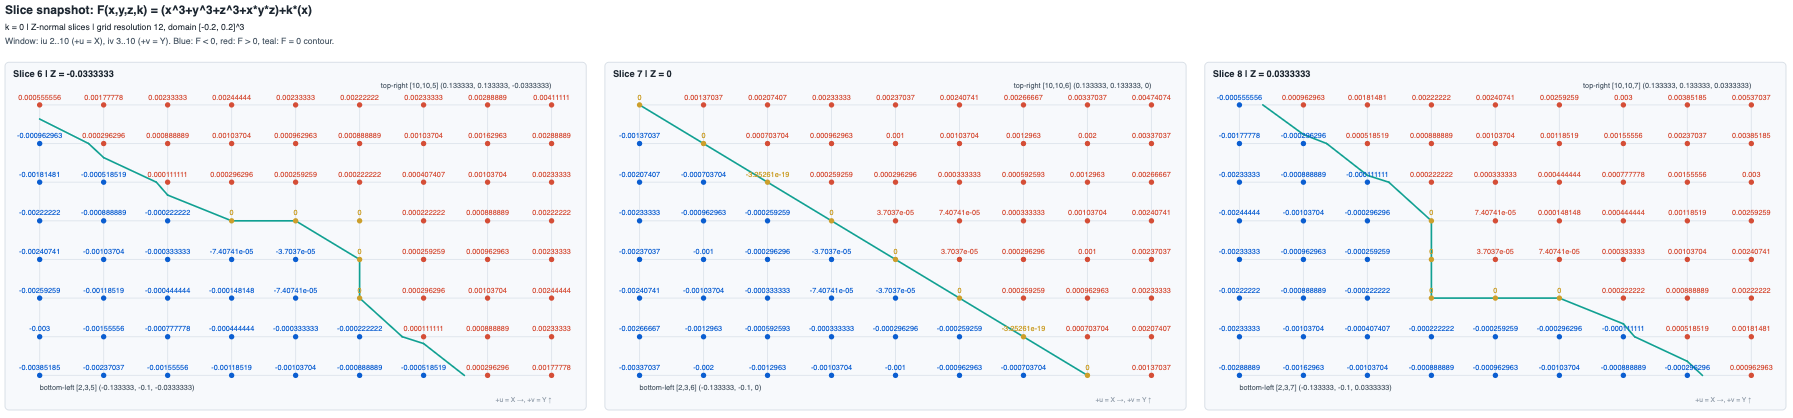
\includegraphics[width=\textwidth]{pictures/report/snap_E6c_k0.png}\\[4pt]
    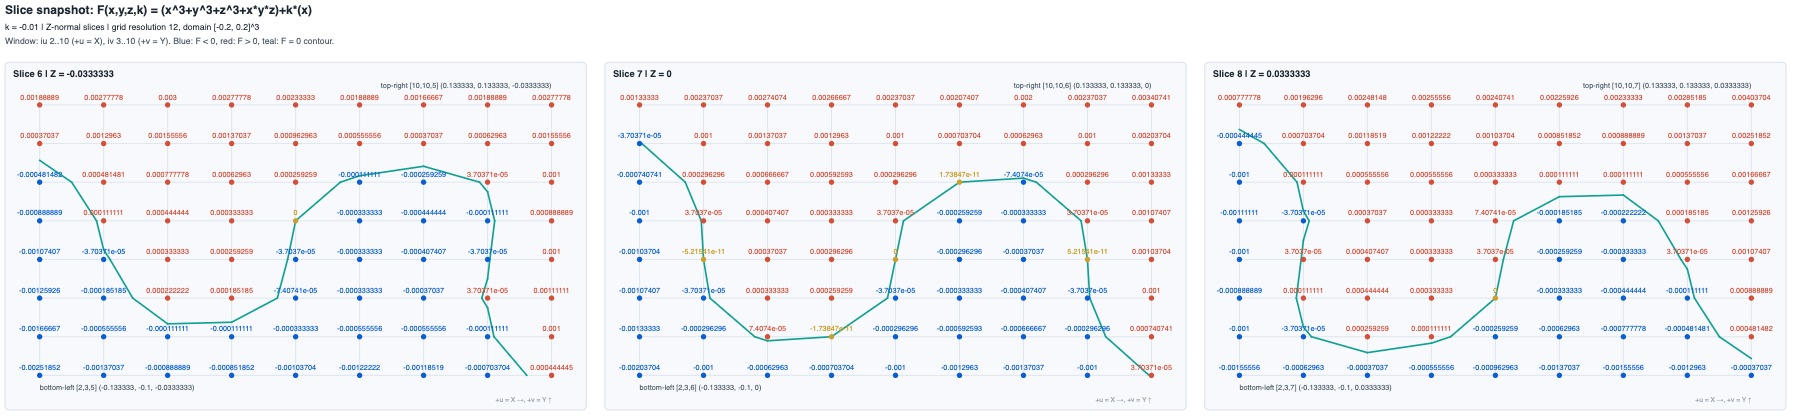
\includegraphics[width=\textwidth]{pictures/report/snap_E6c_kneg.png}\\[4pt]
    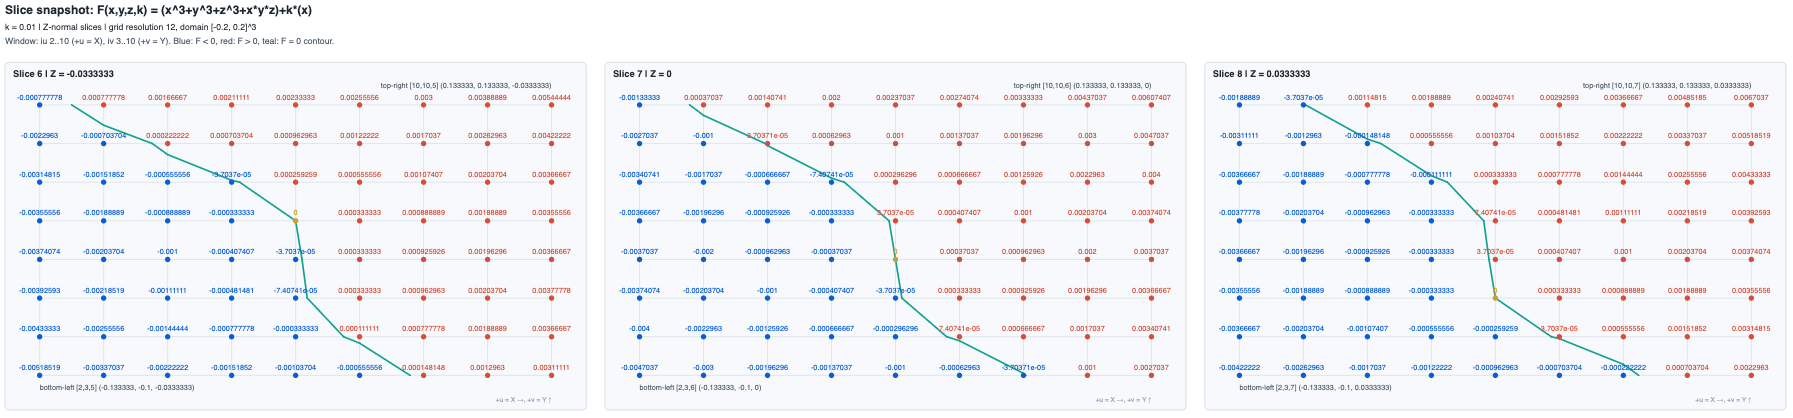
\includegraphics[width=\textwidth]{pictures/report/snap_E6c_kpos.png}
    \caption{Slice snapshots around the singular point of $x^3+y^3+z^3+xyz+kG$ with $G=x$:
    $k=0$ (top), $k<0$ (middle), $k>0$ (bottom); the values of $k$, the grid and
    the window are printed in each snapshot. Every node shows its value (blue
    negative, red positive, yellow zero); teal is the zero level $S_k$.}
    \label{fig:r-E6c-snap}
\end{figure}

\begin{table}[!h]
\centering
\footnotesize
\begin{adjustbox}{max width=\textwidth}
\begin{tabular}{l c l c c c c c c c}
\toprule
& & & & \multicolumn{2}{c}{$k<0$} & \multicolumn{2}{c}{$k>0$} & & \\
\cmidrule(lr){5-6}\cmidrule(lr){7-8}
$G$ & $m$ & essential part & predicted $\alpha$ & $\alpha$ & $C$ & $\alpha$ & $C$ & spread over $N$ & agrees \\
\midrule
$1$ & 0 & $1$ & $\tfrac13$ & 0.334{\scriptsize$\pm$0.001} & 1.03 & 0.334{\scriptsize$\pm$0.001} & 1.03 & 0.003 & yes \\
$x$ & 1 & $x$ & $\tfrac12$ & 0.500{\scriptsize$\pm$0.000} & 0.88 & 0.500{\scriptsize$\pm$0.000} & 0.30 & 0.002 & yes \\
$y$ & 1 & $y$ & $\tfrac12$ & 0.500{\scriptsize$\pm$0.000} & 0.88 & 0.500{\scriptsize$\pm$0.000} & 0.30 & 0.001 & yes \\
$z$ & 1 & $z$ & $\tfrac12$ & 0.500{\scriptsize$\pm$0.000} & 0.88 & 0.500{\scriptsize$\pm$0.000} & 0.30 & 0.001 & yes \\
$x+y$ & 1 & $x + y$ & $\tfrac12$ & 0.500{\scriptsize$\pm$0.000} & 1.15 & 0.500{\scriptsize$\pm$0.000} & 0.44 & 0.001 & yes \\
$x+z$ & 1 & $x + z$ & $\tfrac12$ & 0.500{\scriptsize$\pm$0.000} & 1.15 & 0.500{\scriptsize$\pm$0.000} & 0.44 & 0.001 & yes \\
$x+y+z$ & 1 & $x + y + z$ & $\tfrac12$ & 0.500{\scriptsize$\pm$0.001} & 1.41 & 0.500{\scriptsize$\pm$0.000} & 0.17 & 0.003 & yes \\
$2x-y+3z$ & 1 & $2x - y + 3z$ & $\tfrac12$ & 0.500{\scriptsize$\pm$0.000} & 1.67 & 0.500{\scriptsize$\pm$0.000} & 0.91 & 0.001 & yes \\
$x^2$ & 2 & $-0.333yz$ & $1$ & 1.000{\scriptsize$\pm$0.002} & 0.77 & 1.000{\scriptsize$\pm$0.002} & 0.77 & 0.001 & yes \\
$x^2+y^2-z^2$ & 2 & $y^2 - 0.333yz - z^2$ & $1$ & 1.001{\scriptsize$\pm$0.001} & 0.88 & 1.001{\scriptsize$\pm$0.001} & 0.88 & 0.001 & yes \\
$xy$ & 2 & $-3z^2$ & $1$ & 1.013{\scriptsize$\pm$0.011} & 0.50 & 1.000{\scriptsize$\pm$0.002} & 0.47 & 0.014 & yes \\
$x^3$ & 3 & $z^3$ & $1$ & 1.001{\scriptsize$\pm$0.000} & 0.05 & 0.999{\scriptsize$\pm$0.000} & 0.05 & 0.000 & yes \\
$x^2y+y^2z+z^2x$ & 3 & $0$ & $1$ & 1.000{\scriptsize$\pm$0.000} & 0.05 & 1.000{\scriptsize$\pm$0.000} & 0.05 & 0.000 & yes \\
$x+y+2.0000z$ & 1 & $x + y + 2z$ & $\tfrac12$ & 0.500{\scriptsize$\pm$0.001} & 1.63 & 0.500{\scriptsize$\pm$0.000} & 0.31 & 0.004 & yes \\
$F$ & -- & $0$ & $1$ & $S_k=S_0$ & -- & $S_k=S_0$ & -- & -- & yes \\
\bottomrule
\end{tabular}
\end{adjustbox}
\caption[Rates for $x^3+y^3+z^3+xyz$]{All perturbations of $F=x^3+y^3+z^3+xyz$: convergence rates (resolution $128$). Columns are explained in Section~\ref{sec:r-read}.}
\label{tab:r-E6c-rates}
\end{table}
\begin{table}[!h]
\centering
\footnotesize
\begin{adjustbox}{max width=\textwidth}
\begin{tabular}{l l c l l c}
\toprule
$G$ & $P$ for $k\neq0$ & corank at $P$ & singular points, $k<0$ & singular points, $k>0$ & MC error \\
\midrule
$1$ & leaves $S_k$ & -- & none & none & 0.0004 \\
$x$ & regular & -- & none & none & 0.0029 \\
$y$ & regular & -- & none & none & 0.0026 \\
$z$ & regular & -- & none & none & 0.0031 \\
$x+y$ & regular & -- & none & none & 0.0030 \\
$x+z$ & regular & -- & none & none & 0.0030 \\
$x+y+z$ & regular & -- & none & none & 0.0028 \\
$2x-y+3z$ & regular & -- & none & none & 0.0018 \\
$x^2$ & singular & 2 & only $P$ & only $P$ & 0.0029 \\
$x^2+y^2-z^2$ & singular & 0 ($A_1$) & only $P$ & only $P$ & 0.0042 \\
$xy$ & singular & 1 & only $P$ & only $P$ & 0.0052 \\
$x^3$ & singular & 3 & only $P$ & only $P$ & 0.0026 \\
$x^2y+y^2z+z^2x$ & singular & 3 & only $P$ & only $P$ & 0.0026 \\
$x+y+2.0000z$ & regular & -- & 2$\times$$A_1$, $\gamma=0.50$ & none & 0.0040 \\
$F$ & singular & 3 & only $P$ & only $P$ & 0.0027 \\
\bottomrule
\end{tabular}
\end{adjustbox}
\caption[Singular points for $x^3+y^3+z^3+xyz$]{All perturbations of $F=x^3+y^3+z^3+xyz$: the point $P$, the singular points of $S_k$ and the accuracy of Marching Cubes. Columns are explained in Section~\ref{sec:r-read}.}
\label{tab:r-E6c-points}
\end{table}
\paragraph{Constant ($G=1$).} $0.334$ on both sides, with $C=1.03$.

\paragraph{Linear $G$.} $0.500$ on both sides for every linear $G$, by
self-similarity, as for the Fermat cones; the constants differ a little ($0.88$ for
$k<0$ and $0.30$ for $k>0$ for $G=x$).

\paragraph{Order two and three.} $1.00$ for all of them, and the origin stays
singular. $x^2$ now has the essential part $-\tfrac13yz$ and $xy$ has $-3z^2$: these
are the same directions as for the Fermat cone, written in this cone's basis.

\paragraph{Singular points.} No linear perturbation from the common list creates
singular points: unlike for the Fermat cone, $x+y$ does \emph{not}. The mixed term
$xyz$ moves the directions in which a stationary point lies on the surface. The
direction sweep found the balanced perturbation $x+y+2z$ (to $13$ digits), and it
creates two ordinary double points with $\gamma=0.500$.
\clearpage

\subsection{The cone $x^3+2y^3+3z^3+2xyz$}
\label{sec:r-E6d}

The least symmetric cone: the coefficients differ in every variable. Its
Milnor number is $8$ (computed), which shows that the cubic curve is smooth and
the type is again $\tilde E_6$.

\begin{figure}[!h]
\centering
\begin{minipage}[c]{0.18\textwidth}\centering
      \centering
    \resizebox{\linewidth}{!}{\panel{exact_E6d_k0.png}} \\[2pt]
    {\footnotesize $k=0$}
\end{minipage}\hfill
\begin{minipage}[c]{0.72\textwidth}\centering
\begin{adjustbox}{max width=\textwidth}
\begin{tabular}{c c c}
$G$ & $k=-0.01$ & $k=+0.01$ \\
$1$ & \panel{exact_E6d_1_neg.png} & \panel{exact_E6d_1_pos.png} \\
$x$ & \panel{exact_E6d_x_neg.png} & \panel{exact_E6d_x_pos.png} \\
$x^2+y^2-z^2$ & \panel{exact_E6d_x2py2mz2_neg.png} & \panel{exact_E6d_x2py2mz2_pos.png} \\
\end{tabular}
\end{adjustbox}
\end{minipage}
\caption{Exact slices of $S_k$ on the plane $z=0$ (horizontal axis $x$, vertical
axis $y$, both from $-0.25$ to $0.25$), computed from the polynomial. Grey: the
singular surface $S_0$; blue: $S_k$; red: singular points of $S_k$ found by the
numerical stationary-point search; cross: the origin.}
\label{fig:r-E6d-exact}
\end{figure}

\begin{figure}[!h]
    \centering
    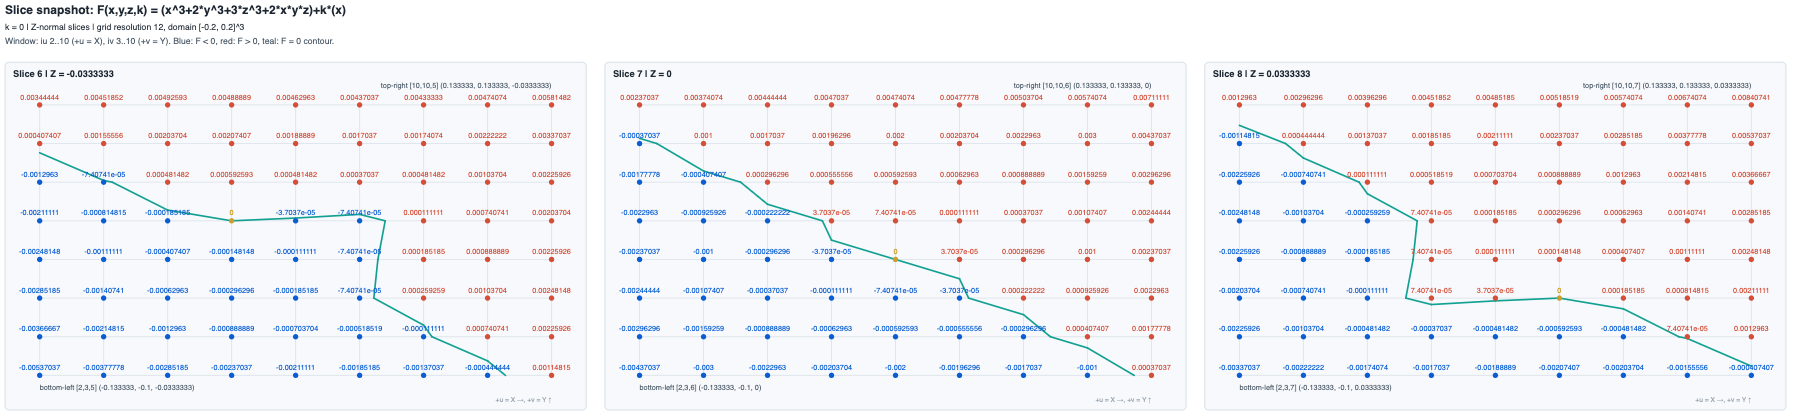
\includegraphics[width=\textwidth]{pictures/report/snap_E6d_k0.png}\\[4pt]
    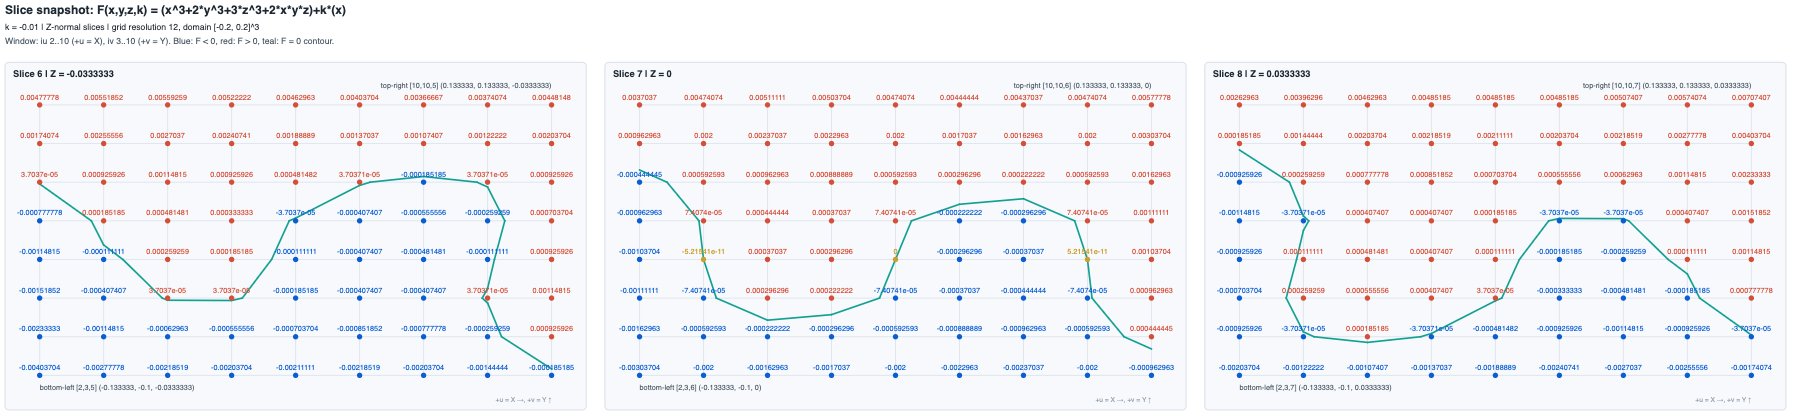
\includegraphics[width=\textwidth]{pictures/report/snap_E6d_kneg.png}\\[4pt]
    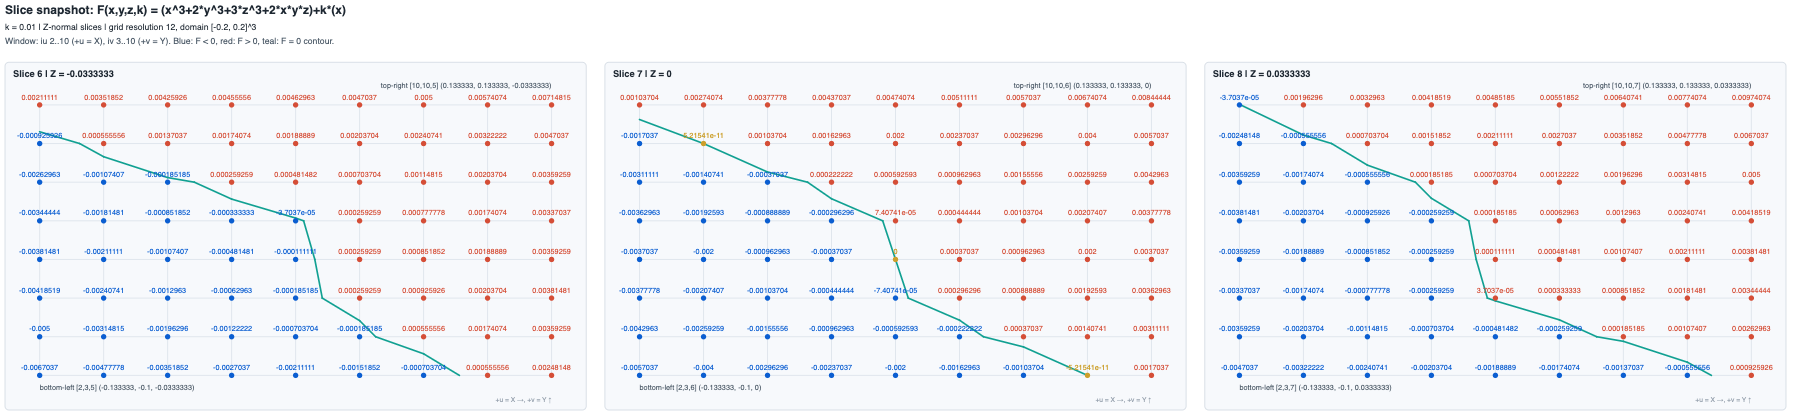
\includegraphics[width=\textwidth]{pictures/report/snap_E6d_kpos.png}
    \caption{Slice snapshots around the singular point of $x^3+2y^3+3z^3+2xyz+kG$ with $G=x$:
    $k=0$ (top), $k<0$ (middle), $k>0$ (bottom); the values of $k$, the grid and
    the window are printed in each snapshot. Every node shows its value (blue
    negative, red positive, yellow zero); teal is the zero level $S_k$.}
    \label{fig:r-E6d-snap}
\end{figure}

\begin{table}[!h]
\centering
\footnotesize
\begin{adjustbox}{max width=\textwidth}
\begin{tabular}{l c l c c c c c c c}
\toprule
& & & & \multicolumn{2}{c}{$k<0$} & \multicolumn{2}{c}{$k>0$} & & \\
\cmidrule(lr){5-6}\cmidrule(lr){7-8}
$G$ & $m$ & essential part & predicted $\alpha$ & $\alpha$ & $C$ & $\alpha$ & $C$ & spread over $N$ & agrees \\
\midrule
$1$ & 0 & $1$ & $\tfrac13$ & 0.334{\scriptsize$\pm$0.001} & 0.83 & 0.334{\scriptsize$\pm$0.001} & 0.83 & 0.001 & yes \\
$x$ & 1 & $x$ & $\tfrac12$ & 0.500{\scriptsize$\pm$0.001} & 0.69 & 0.500{\scriptsize$\pm$0.000} & 0.27 & 0.001 & yes \\
$y$ & 1 & $y$ & $\tfrac12$ & 0.501{\scriptsize$\pm$0.001} & 0.61 & 0.501{\scriptsize$\pm$0.000} & 0.25 & 0.001 & yes \\
$z$ & 1 & $z$ & $\tfrac12$ & 0.501{\scriptsize$\pm$0.002} & 0.59 & 0.500{\scriptsize$\pm$0.000} & 0.21 & 0.001 & yes \\
$x+y$ & 1 & $x + y$ & $\tfrac12$ & 0.500{\scriptsize$\pm$0.000} & 0.82 & 0.500{\scriptsize$\pm$0.000} & 0.31 & 0.001 & yes \\
$x+z$ & 1 & $x + z$ & $\tfrac12$ & 0.500{\scriptsize$\pm$0.001} & 0.84 & 0.500{\scriptsize$\pm$0.000} & 0.33 & 0.002 & yes \\
$x+y+z$ & 1 & $x + y + z$ & $\tfrac12$ & 0.500{\scriptsize$\pm$0.000} & 0.97 & 0.500{\scriptsize$\pm$0.000} & 0.16 & 0.001 & yes \\
$2x-y+3z$ & 1 & $2x - y + 3z$ & $\tfrac12$ & 0.501{\scriptsize$\pm$0.001} & 1.20 & 0.500{\scriptsize$\pm$0.000} & 0.67 & 0.001 & yes \\
$x^2$ & 2 & $-0.666yz$ & $1$ & 1.015{\scriptsize$\pm$0.011} & 0.68 & 1.003{\scriptsize$\pm$0.004} & 0.64 & 0.006 & yes \\
$x^2+y^2-z^2$ & 2 & $y^2 - 0.666yz - z^2$ & $1$ & 1.013{\scriptsize$\pm$0.010} & 0.66 & 1.003{\scriptsize$\pm$0.005} & 0.62 & 0.008 & yes \\
$xy$ & 2 & $-4.5z^2$ & $1$ & 1.043{\scriptsize$\pm$0.043} & 0.34 & 1.003{\scriptsize$\pm$0.003} & 0.27 & 0.017 & yes \\
$x^3$ & 3 & $3z^3$ & $1$ & 1.001{\scriptsize$\pm$0.000} & 0.04 & 0.999{\scriptsize$\pm$0.000} & 0.04 & 0.000 & yes \\
$x^2y+y^2z+z^2x$ & 3 & $0$ & $1$ & 1.000{\scriptsize$\pm$0.000} & 0.03 & 1.000{\scriptsize$\pm$0.000} & 0.03 & 0.002 & yes \\
$x+y+2.6581z$ & 1 & $x + y + 2.658z$ & $\tfrac12$ & 0.500{\scriptsize$\pm$0.000} & 1.20 & 0.500{\scriptsize$\pm$0.000} & 0.26 & 0.000 & yes \\
$F$ & -- & $0$ & $1$ & $S_k=S_0$ & -- & $S_k=S_0$ & -- & -- & yes \\
\bottomrule
\end{tabular}
\end{adjustbox}
\caption[Rates for $x^3+2y^3+3z^3+2xyz$]{All perturbations of $F=x^3+2y^3+3z^3+2xyz$: convergence rates (resolution $128$). Columns are explained in Section~\ref{sec:r-read}.}
\label{tab:r-E6d-rates}
\end{table}
\begin{table}[!h]
\centering
\footnotesize
\begin{adjustbox}{max width=\textwidth}
\begin{tabular}{l l c l l c}
\toprule
$G$ & $P$ for $k\neq0$ & corank at $P$ & singular points, $k<0$ & singular points, $k>0$ & MC error \\
\midrule
$1$ & leaves $S_k$ & -- & none & none & 0.0005 \\
$x$ & regular & -- & none & none & 0.0032 \\
$y$ & regular & -- & none & none & 0.0039 \\
$z$ & regular & -- & none & none & 0.0053 \\
$x+y$ & regular & -- & none & none & 0.0038 \\
$x+z$ & regular & -- & none & none & 0.0048 \\
$x+y+z$ & regular & -- & none & none & 0.0045 \\
$2x-y+3z$ & regular & -- & none & none & 0.0033 \\
$x^2$ & singular & 2 & only $P$ & only $P$ & 0.0031 \\
$x^2+y^2-z^2$ & singular & 0 ($A_1$) & only $P$ & only $P$ & 0.0033 \\
$xy$ & singular & 1 & only $P$ & only $P$ & 0.0032 \\
$x^3$ & singular & 3 & only $P$ & only $P$ & 0.0030 \\
$x^2y+y^2z+z^2x$ & singular & 3 & only $P$ & only $P$ & 0.0030 \\
$x+y+2.6581z$ & regular & -- & 2$\times$$A_1$, $\gamma=0.50$ & none & 0.0032 \\
$F$ & singular & 3 & only $P$ & only $P$ & 0.0030 \\
\bottomrule
\end{tabular}
\end{adjustbox}
\caption[Singular points for $x^3+2y^3+3z^3+2xyz$]{All perturbations of $F=x^3+2y^3+3z^3+2xyz$: the point $P$, the singular points of $S_k$ and the accuracy of Marching Cubes. Columns are explained in Section~\ref{sec:r-read}.}
\label{tab:r-E6d-points}
\end{table}
\paragraph{Constant ($G=1$).} $0.334$ on both sides. The constant $C=0.83$ is the
smallest of the four cones: the larger coefficients make $F$ larger at the same
distance from $P$, so the same $k$ moves the surface less.

\paragraph{Linear $G$.} $0.500$ on both sides for every linear $G$; for $G=x$ the
constants are $0.69$ ($k<0$) and $0.27$ ($k>0$).

\paragraph{Order two and three.} $1.00$ for all of them, and the origin stays
singular. The essential parts are again the same directions written in this cone's
basis ($-0.666\,yz$ for $x^2$, $-4.5\,z^2$ for $xy$).

\paragraph{Singular points.} None from the common list. The direction sweep found
the balanced direction $x+y+2.6581z$, which creates two ordinary double points with
$\gamma=0.500$; without the sweep there would be no way to guess this coefficient.
\clearpage

% =============================================================================
\section{Surfaces That Behave Alike}
\label{sec:r-groupF}
% =============================================================================

Looking at all ten surfaces together, they fall into five groups. Within a group
the rates are the same for the same perturbation; between groups they differ, and
the reason is always the local type together with the real shape near $P$.

\begin{table}[!h]
\centering
\small
\begin{adjustbox}{max width=\textwidth}
\begin{tabular}{l l c c c c}
\toprule
group & surfaces & $G=1$ & essential linear & inessential linear & order $\ge2$ \\
\midrule
I cubic cones & $x^3+y^3\pm z^3$, $x^3+y^3+z^3+xyz$, & $\tfrac13$ & $\tfrac12$ (both sides) & -- & $1$ \\
 & $x^3+2y^3+3z^3+2xyz$ & & & & \\
II double point & $x^2+y^2-z^2+xyz$ & $\tfrac12$ & -- & $1$ & $1$ \\
III horn cusps & $x^2+y^2+z^3$, $x^3+y^3+z^2+x^2$ & $\tfrac13$ & $\tfrac12$ / $\tfrac34$ & $\tfrac23$ (spike) & $1$ \\
IV saddle cusp & $x^2-y^2+z^3$ & $\tfrac12$ & $\tfrac34$ (both sides) & $\approx0.93$ & $1$ \\
V $D_4$ & $x^2+y^3+z^3$, $x^2+y^3-3yz^2$ & $\tfrac13$ & $\tfrac12$ & $0.68$--$0.76$ & $1$ \\
\bottomrule
\end{tabular}
\end{adjustbox}
\caption{Typical measured rates per group ($k<0$ / $k>0$ where they differ).
``--'': no such perturbation in the list (for the cones every linear $G$ is
essential, for $A_1$ none is).}
\label{tab:r-groups}
\end{table}

\paragraph{Group I: the cubic cones.} Same rates, exactly: $\tfrac13$, $\tfrac12$,
$1$ for $m=0,1,\ge2$, on both sides, independent of the grid. The reason is
self-similarity: $F$ is homogeneous, so near $P$ the surface is a fixed shape
scaled by $\lambda(k)$. The four cones differ only in the constants $C$ and in
\emph{which} linear perturbations create singular points: for the Fermat cones
$x+y$ does, for the other two it does not, and each has its own balanced direction.
The algebraic type ($\tilde E_6$) fixes the rates; the actual cubic curve fixes the
singular points.

\paragraph{Group II: the double point.} Only the constant term is essential, so
only $G=1$ opens the cone at first order, at the scale $\sqrt{|k|}$
($\alpha=\tfrac12$). Everything else moves the cone by a distance proportional to $|k|$ ($\alpha=1$).

\paragraph{Group III: the horn cusps.} $x^2+y^2+z^3$ and $x^3+y^3+z^2+x^2$ are the
same singularity with the horn along $z$ and along $y$, and they give the same
numbers once $y$ and $z$ are exchanged (the term $x^3$ does not matter near $P$).
The constant moves the tip along the horn ($\tfrac13$); the essential direction
splits the horn for one sign of $k$ ($\tfrac12$) and only thickens it for the other
($\tfrac34$); inessential directions create the thin spike ($\tfrac23$).

\paragraph{Group IV: the saddle cusp.} $x^2-y^2+z^3$ has the same algebraic type as
group III, but its quadratic part is a saddle. The constant opens the two crossing
sheets sideways ($\tfrac12$ instead of $\tfrac13$), there is no spike ($0.93$
instead of $\tfrac23$), and $x+y$ moves the cusp instead of opening it. The sign
pattern of the quadratic part changes the real geometry, and with it the rates,
even though the complex type is the same.

\paragraph{Group V: the $D_4$ points.} Rates $\tfrac13$ and $\tfrac12$, the lower
ends of the ranges. The two surfaces differ in the number of real lines of their
cubic part. With one line ($x^2+y^3+z^3$) the constants differ strongly between
$k<0$ and $k>0$; with three lines ($x^2+y^3-3yz^2$) both sides look alike, and
$G=y$ creates two ordinary double points.

% =============================================================================
\section{Perturbations That Behave Alike}
\label{sec:r-groupG}
% =============================================================================

The same grouping works for the perturbations. What matters is the order of $G$
and whether its lowest part is essential.

\begin{description}
    \item[Constant ($G=1$).] $P$ leaves the surface, no singular points anywhere
          near $P$. Rate $\tfrac13$ (cones, horn cusps, $D_4$) or $\tfrac12$ (double
          point, saddle cusp): the tip moves along the direction of smallest weight,
          or the sheets open sideways.
    \item[Essential linear ($x,y,z,x+y,\dots$ for the cones; $z$ for $x^2\pm y^2+z^3$;
          $y,z$ for $D_4$).] $P$ becomes regular; the singularity is opened at the
          scale $\sqrt{|k|}$ on at least one side. Singular points appear only for
          special directions: those satisfying the balance condition for the cones,
          $y$ for the three-line $D_4$.
    \item[Inessential linear ($x$, $y$ for the cusps; $x$ for $D_4$; every linear
          $G$ for $A_1$).] $P$ becomes regular, but the surface is mainly shifted.
          The genuine change comes at second order in $k$: a spike for the horn
          cusp ($\tfrac23$), a shift for the others (close to $1$). For the saddle cusp,
          $x+y$ even moves the singular point along ($\gamma=1$).
    \item[Mixed linear ($x+z$, $x+y+z$, $2x-y+3z$ on cusps and $D_4$).] They have an
          essential and an inessential part. The essential part decides the rate
          for small $|k|$; the inessential shift adds a contribution of order $|k|$
          that pushes the measured rate up for the side with the slower essential
          rate (the deviations above $\tfrac34$).
    \item[Order two ($x^2$, $x^2+y^2-z^2$, $xy$).] $P$ stays singular; the surface is
          deformed by $O(|k|)$, $\alpha=1$. The type at $P$ becomes simpler or stays:
          $x^2+y^2-z^2$ always produces an ordinary double point (corank $0$), and on
          the Fermat cones and on $x^2+y^3+z^3$ it creates additional ordinary double
          points moving with $\gamma=1$.
    \item[Order three ($x^3$, $x^2y+y^2z+z^2x$).] $P$ stays singular with the same
          type; the surface is stretched or bent by $O(|k|)$ with very small
          constants ($\le0.05$).
    \item[$G=F$.] $H_k=(1+k)F$, so $S_k=S_0$: the measured distance is zero for every
          $k$ (below $10^{-12}$), a check of the measurement.
    \item[Balanced.] Constructed to create singular points: two ordinary double
          points moving with $\gamma=\tfrac12$ for $k<0$, on all four cones.
\end{description}

\paragraph{Overview of all pairs.} Table~\ref{tab:summary} counts, for each
surface, how many rates were fitted, how many agree with the prediction, and how
for how many values of $k$ the stationary-point search was consistent with the expected Milnor-number count. Table~\ref{tab:singular-created}
lists every pair in which singular points other than $P$ appear.

\begin{table}[!h]
\centering
\small
\begin{adjustbox}{max width=\textwidth}
\begin{tabular}{l l c c c c}
\toprule
Type & $F$ & fitted sides & within prediction & $\mu$-consistent $k$ & surfaces with singular points \\
\midrule
$A_1$ & $x^2+y^2-z^2+xyz$ & 26 & 26 & 252/252 & 0 \\
$A_2$ & $x^2+y^2+z^3$ & 26 & 23 & 252/252 & 0 \\
$A_2$ & $x^2-y^2+z^3$ & 26 & 23 & 252/252 & 1 \\
$A_2$ & $x^3+y^3+z^2+x^2$ & 26 & 23 & 252/252 & 0 \\
$D_4$ & $x^2+y^3+z^3$ & 26 & 23 & 252/252 & 1 \\
$D_4$ & $x^2+y^3-3yz^2$ & 26 & 23 & 252/252 & 1 \\
$\tilde E_6$ & $x^3+y^3+z^3$ & 28 & 28 & 270/270 & 4 \\
$\tilde E_6$ & $x^3+y^3-z^3$ & 28 & 28 & 270/270 & 3 \\
$\tilde E_6$ & $x^3+y^3+z^3+xyz$ & 28 & 28 & 270/270 & 1 \\
$\tilde E_6$ & $x^3+2y^3+3z^3+2xyz$ & 28 & 28 & 270/270 & 1 \\
\midrule
all & & 268 & 253 & 2592/2592 & \\
\bottomrule
\end{tabular}
\end{adjustbox}
\caption[Summary of all experiments]{Summary of all perturbations at resolution $128$. ``Fitted sides'': sides $k<0$, $k>0$ with a rate fit (excluding $G=F$); ``within prediction'': the $95\%$ confidence interval meets the predicted range \eqref{eq:r-alpha} widened by $0.02$; ``$\mu$-consistent $k$'': values of $k$ for which the total multiplicity of the computed stationary points is consistent with the expected Milnor-number count; last column: number of perturbations $G$ for which $S_k$ has singular points moving into the origin.}
\label{tab:summary}
\end{table}

\begin{table}[!h]
\centering
\footnotesize
\begin{adjustbox}{max width=\textwidth}
\begin{tabular}{l l l l l}
\toprule
Type & $F$ & $G$ & $k<0$ & $k>0$ \\
\midrule
$A_2$ & $x^2-y^2+z^3$ & $x+y$ & 1$\times$$A_2$, $\gamma{=}1.00$ & 1$\times$$A_2$, $\gamma{=}1.00$ \\
$A_2$ & $x^3+y^3+z^2+x^2$ & $xy$ & some $k$ & some $k$ \\
$D_4$ & $x^2+y^3+z^3$ & $x^2+y^2-z^2$ & $P$ + 1$\times$$A_1$, $\gamma{=}1.00$ & $P$ + 1$\times$$A_1$, $\gamma{=}1.00$ \\
$D_4$ & $x^2+y^3+z^3$ & $xy$ & some $k$ & some $k$ \\
$D_4$ & $x^2+y^3-3yz^2$ & $y$ & none & 2$\times$$A_1$, $\gamma{=}0.50$ \\
$D_4$ & $x^2+y^3-3yz^2$ & $xy$ & some $k$ & some $k$ \\
$\tilde E_6$ & $x^3+y^3+z^3$ & $x+y$ & 2$\times$$A_2$, $\gamma{=}0.50$ & none \\
$\tilde E_6$ & $x^3+y^3+z^3$ & $x+z$ & 2$\times$$A_2$, $\gamma{=}0.50$ & none \\
$\tilde E_6$ & $x^3+y^3+z^3$ & $x^2+y^2-z^2$ & $P$ + 2$\times$$A_1$, $\gamma{=}1.00$ & $P$ + 2$\times$$A_1$, $\gamma{=}1.00$ \\
$\tilde E_6$ & $x^3+y^3+z^3$ & $x+y+1.5874010519681567z$ & 2$\times$$A_1$, $\gamma{=}0.50$ & none \\
$\tilde E_6$ & $x^3+y^3-z^3$ & $x+y$ & 2$\times$$A_2$, $\gamma{=}0.50$ & none \\
$\tilde E_6$ & $x^3+y^3-z^3$ & $x^2+y^2-z^2$ & $P$ + 2$\times$$A_1$, $\gamma{=}1.00$ & $P$ + 2$\times$$A_1$, $\gamma{=}1.00$ \\
$\tilde E_6$ & $x^3+y^3-z^3$ & $x+y-1.5874010519682413z$ & 2$\times$$A_1$, $\gamma{=}0.50$ & none \\
$\tilde E_6$ & $x^3+y^3+z^3+xyz$ & $x+y+1.9999999999999403z$ & 2$\times$$A_1$, $\gamma{=}0.50$ & none \\
$\tilde E_6$ & $x^3+2y^3+3z^3+2xyz$ & $x+y+2.6580633932167901z$ & 2$\times$$A_1$, $\gamma{=}0.50$ & none \\
\bottomrule
\end{tabular}
\end{adjustbox}
\caption[Created singular points]{All perturbations for which $S_k$ has singular points other than a persistent singular point at the origin (resolution $128$; all computed multiplicity totals matched the Milnor-number count). Notation as in Section~\ref{sec:r-read}; ``some $k$'': singular points found only for some values of $k$ (see text).}
\label{tab:singular-created}
\end{table}

\subsection{The direction sweep}
\label{sec:r-sweep}

The common list contains only a few linear perturbations, and for the cones it
misses the directions $c$ of $G=c_1x+c_2y+c_3z$ for which $S_k$ becomes singular.
These were searched for numerically: for many directions $c$ the real stationary
points $q$ of $H_k$ were computed, and a direction was marked where some $q$ also
satisfies $H_k(q)=0$ (Section~\ref{sec:r-method}). The search found the balanced
perturbations $x+y\pm1.5874z$, $x+y+2z$ and $x+y+2.6581z$ of
Table~\ref{tab:singular-created}.

For $x^3+y^3+z^3$ the result can be checked by hand. Take $G=x+y+cz$ with $c\ge0$
and $k<0$. By the formula of Section~\ref{sec:r-E6a}, the stationary points are real,
and the value of $H_k$ at them is, up to the factor $\tfrac{2}{3}|k|^{3/2}/\sqrt3$,
one of the numbers $\pm1\pm1\pm c^{3/2}$. The smallest of their absolute values,
\[
m(c)=\min\big(|2-c^{3/2}|,\ c^{3/2}\big),
\]
measures how far the nearest stationary point is from lying on the surface.
Figure~\ref{fig:r-sweep} shows $m(c)$. $S_k$ is singular exactly where $m(c)=0$:
at $c=0$ ($G=x+y$, two cusps) and at $c=2^{2/3}\approx1.5874$ (the balanced
perturbation, two ordinary double points). Every other $c$, for example $c=1$
($G=x+y+z$), gives a smooth $S_k$. A small change of the direction moves the
stationary points off the surface, which is why such directions are found only by a
search, and why the common list, which was written down without it, contains only
$x+y$.

\begin{figure}[!h]
\centering
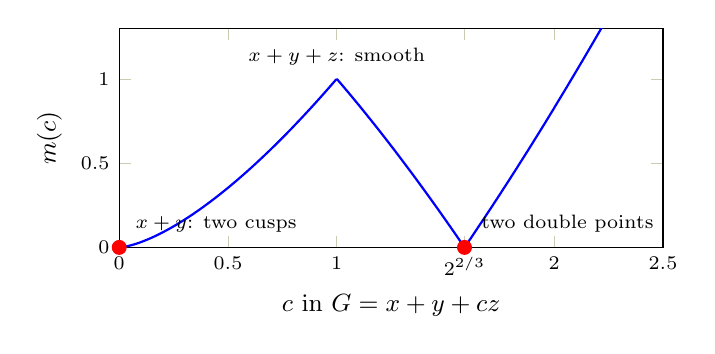
\begin{tikzpicture}
\begin{axis}[width=0.7\textwidth, height=0.36\textwidth, xmin=0, xmax=2.5, ymin=0, ymax=1.3,
    xlabel={$c$ in $G=x+y+cz$}, ylabel={$m(c)$}, tick label style={font=\scriptsize},
    label style={font=\small}, xtick={0,0.5,1,1.5874,2,2.5},
    xticklabels={$0$,$0.5$,$1$,$2^{2/3}$,$2$,$2.5$}]
\addplot[blue, thick, domain=0:2.5, samples=400] {min(abs(2-x^1.5), x^1.5)};
\addplot[only marks, mark=*, red, mark size=2.5pt] coordinates {(0,0) (1.5874,0)};
\node[anchor=south west, font=\scriptsize] at (axis cs:0.03,0.03) {$x+y$: two cusps};
\node[anchor=south west, font=\scriptsize] at (axis cs:1.62,0.03) {two double points};
\node[anchor=south, font=\scriptsize] at (axis cs:1,1.02) {$x+y+z$: smooth};
\end{axis}
\end{tikzpicture}
\caption{Perturbations $G=x+y+cz$ of $x^3+y^3+z^3$ with $k<0$: the distance $m(c)$ of
the nearest stationary point from lying on the surface (in units of
$\tfrac{2}{3\sqrt3}|k|^{3/2}$). $S_k$ is singular exactly at the zeros (red).}
\label{fig:r-sweep}
\end{figure}

% =============================================================================
\section{How Well Marching Cubes Sees the Singular Point}
\label{sec:r-accuracy}
% =============================================================================

Away from the singular points Marching Cubes \cite{lorensen1998marching,wenger2013} does what it should: the median
extraction error is about a quarter of a grid cell and halves when the grid is
refined (Table~\ref{tab:extraction-error}). The problems are local, and the
experiments show two of them.

\begin{itemize}
    \item \textbf{Thin features disappear.} The spike of $x^2+y^2+z^3+kx$ is
          narrower than a cell for every tested $k$; the mesh does not contain it,
          and the extraction error is caused by the missing spike ($0.0201$, more
          than three cells, in Table~\ref{tab:r-A2a-points}; the same happens for
          $x^2+y^3+z^3+kx$, $0.0226$ in Table~\ref{tab:r-D4a-points}). Every mesh point is still close to
          the surface; only the comparison from the surface to the mesh reveals the
          missing part.
    \item \textbf{Singular points that are not grid nodes are not in the mesh.} The
          singular point $P$ is a grid node, so the mesh contains it. The singular
          points that move with $k$ are not: for the balanced perturbation of
          $x^3+y^3+z^3$ the double points are up to $0.0106$ (half a cell) away from
          the mesh at $N=32$, $0.0064$ at $N=64$ and $0.0016$ at $N=128$. The mesh
          passes near them but triangulates as if the surface were smooth there.
\end{itemize}
The snapshots show the same on the grid itself: in Figure~\ref{fig:r-D4b-snap} the
two double points at $z=\pm0.037$ lie between grid planes, so no node of the grid is
singular.

\begin{table}[!h]
\centering
\small
\begin{adjustbox}{max width=\textwidth}
\begin{tabular}{l c c c c c}
\toprule
Type & $F$ & $N=32$ & $N=64$ & $N=128$ & order \\
\midrule
$A_1$ & $x^2+y^2-z^2+xyz$ & 5.55e-03 & 2.76e-03 & 1.39e-03 & 0.99 \\
$A_2$ & $x^2+y^2+z^3$ & 7.98e-03 & 4.11e-03 & 2.11e-03 & 0.96 \\
$A_2$ & $x^2-y^2+z^3$ & 5.87e-03 & 2.93e-03 & 1.48e-03 & 0.98 \\
$A_2$ & $x^3+y^3+z^2+x^2$ & 8.05e-03 & 4.14e-03 & 2.11e-03 & 0.97 \\
$D_4$ & $x^2+y^3+z^3$ & 6.13e-03 & 3.13e-03 & 1.53e-03 & 1.03 \\
$D_4$ & $x^2+y^3-3yz^2$ & 1.09e-02 & 5.37e-03 & 2.34e-03 & 1.20 \\
$\tilde E_6$ & $x^3+y^3+z^3$ & 7.18e-03 & 3.52e-03 & 1.69e-03 & 1.06 \\
$\tilde E_6$ & $x^3+y^3-z^3$ & 7.19e-03 & 3.57e-03 & 1.57e-03 & 1.18 \\
$\tilde E_6$ & $x^3+y^3+z^3+xyz$ & 1.02e-02 & 4.07e-03 & 1.67e-03 & 1.28 \\
$\tilde E_6$ & $x^3+2y^3+3z^3+2xyz$ & 1.21e-02 & 5.78e-03 & 2.00e-03 & 1.53 \\
\bottomrule
\end{tabular}
\end{adjustbox}
\caption[Extraction error]{Median extraction error of the Marching Cubes meshes (Hausdorff distance between the mesh and the exact surface in the box, Section~\ref{sec:r-method}) over all perturbations and values of $k$, for the three resolutions; ``order'' is $\log_2$ of the ratio between $N=64$ and $N=128$.}
\label{tab:extraction-error}
\end{table}

% =============================================================================
\section{Where the Results Deviate}
\label{sec:r-deviations}
% =============================================================================

Of $268$ fitted rates, $15$ have a confidence interval that misses the prediction.

\paragraph{Two effects at once (10 cases).} On the cusps and on $D_4$, the
perturbations $x+z$, $x+y+z$, $2x-y+3z$ (and $x+y$ on $x^3+y^3+z^2+x^2$) have an
essential part that deforms the surface at the scale $|k|^{3/4}$ and an
inessential part that shifts it by $O(|k|)$. Over $10^{-4}\le|k|\le10^{-2}$ both
are visible, and the log--log line bends; the fitted slopes $0.77$--$0.88$ lie
between the two rates. The confidence interval is narrow because the points
scatter little, not because the line is straight. For smaller $|k|$ the essential
part would win and the rate would approach $\tfrac34$.

\paragraph{Below the resolution of the measurement (5 cases).} On the two $D_4$
surfaces, $xy$, $x^2+y^2-z^2$ and $x^2y+y^2z+z^2x$ deform the surface by
$|k|\cdot10^{-4}$ or less. The measured distance levels off at about
$1.5\cdot10^{-4}$: at a $D_4$ point the gradient vanishes to second order in two
directions, and the closest-point equations become nearly singular. These fitted
rates ($0.17$--$0.63$) describe the measurement, not the surfaces.

\paragraph{A resolution limit of the singular-point search.} For $G=xy$ on
$x^2+y^3+z^3$, $x^2+y^3-3yz^2$ and $x^3+y^3+z^2+x^2$, a second stationary point lies at
distance $\approx k^2/6$ from $P$ with the value $\approx-k^6/432$. For most $|k|$
it is closer to $P$ than the grouping radius $10^{-5}$, and its value is far below
any tolerance, so it is reported as singular only for some $k$. Exactly, it is not
singular. The count of stationary points is still complete.

% =============================================================================
\section{Reconstructing $S_0$ by Linear Interpolation}
\label{sec:r-interp}
% =============================================================================

The previous sections show that $S_k$ approaches $S_0$ as $k\to0$. Here we ask
a different question: \emph{can the singular surface $S_0$ be reconstructed by
linearly interpolating between the two perturbed surfaces $S_{-\varepsilon}$ and
$S_{+\varepsilon}$?} The motivation is practical. Near $P$ the surfaces
$S_{\pm\varepsilon}$ are often smooth and are extracted well by Marching Cubes,
while $S_0$ is not. If the ``average'' of $S_{-\varepsilon}$ and
$S_{+\varepsilon}$ were much closer to $S_0$ than either of them, one could compute
the singular surface from two regular ones.

\subsection{What can be interpolated}
\label{sec:r-interp-methods}

\paragraph{The implicit functions.} Because $H_k=F+kG$ depends linearly on $k$,
\[
\tfrac12\big(H_{-\varepsilon}+H_{+\varepsilon}\big)=F
\]
exactly, for every $\varepsilon$ and every $G$. On the voxel grid this means: if every
node gets the value $\tfrac12H_{-\varepsilon}+\tfrac12H_{+\varepsilon}$, it gets
exactly the value of $F$ (the program checks this; the largest difference is
$3\cdot10^{-17}$, rounding error), and Marching Cubes produces exactly the mesh of
$F$, triangle for triangle. This averaging is therefore not wrong. It is the best
reconstruction that the grid values allow, and it keeps the singular point, because
$S_0$ has it. But it is not better than extracting $S_0$ directly, and near $P$ the
direct mesh has the defects of Section~\ref{sec:r-accuracy}: an error of about a
third of a cell and, for $x^2+y^2-z^2+xyz$ and $x^2+y^3-3yz^2$, the wrong topology
(Section~\ref{sec:r-cone}). To do better near $P$, the extraction itself has to
change there; Section~\ref{sec:r-cone} does this.

The question of this section is therefore whether the \emph{geometry} can be
interpolated, i.e.\ whether $S_0$ can be obtained when only the two surfaces (their
meshes or their distance fields) are known. We compare four reconstructions:
\begin{description}
    \item[Vertex interpolation (mesh).] Every vertex $v$ of the mesh of
          $S_{-\varepsilon}$ is paired with the closest point $c(v)$ of the mesh of
          $S_{+\varepsilon}$ and moved to the midpoint $\tfrac12(v+c(v))$; the
          triangles of the mesh of $S_{-\varepsilon}$ are kept. The same is done
          starting from $S_{+\varepsilon}$. The closest point is used as the
          correspondence because two independently extracted meshes have no common
          vertex numbering. In the tables the worse of the two directions is given.
    \item[Vertex interpolation (exact).] The same on the exact surfaces: $v$ is
          first moved to the closest point of the exact $S_{-\varepsilon}$, $c(v)$ is
          the closest point of the exact $S_{+\varepsilon}$ (both computed as in
          Section~\ref{sec:r-method}). This removes the extraction error of the two
          meshes and measures the error of the interpolation itself.
    \item[Distance-field interpolation (SDF).] With $\varphi_\pm(p)$ the signed
          distance from $p$ to the mesh of $S_{\pm\varepsilon}$ (sign from the grid
          values of $H_{\pm\varepsilon}$), the reconstruction is the zero level of
          $\tfrac12(\varphi_-+\varphi_+)$, extracted by Marching Cubes on the same
          grid. It is the set of points that lie ``halfway'' between the two
          surfaces, and unlike vertex interpolation it may have a different topology
          than either of them.
    \item[Endpoints.] For comparison: the meshes of $S_{-\varepsilon}$ and
          $S_{+\varepsilon}$ themselves (no interpolation), and the direct Marching
          Cubes mesh of $F$.
\end{description}

\subsection{What to expect}
\label{sec:r-interp-theory}

\paragraph{Away from $P$: second order.} Near a regular point $p_0$ of $S_0$ with
unit normal $n=\nabla F/\|\nabla F\|$, the surface $S_k$ is a graph over $S_0$ in
the normal direction, $p_0+s(k)n$, and expanding $F(p_0+sn)+kG(p_0+sn)=0$ gives
\[
s(k)=-k\,\frac{G(p_0)}{\|\nabla F(p_0)\|}+c\,k^2+O(k^3).
\]
The first-order term is odd in $k$ and cancels in the midpoint:
$\tfrac12\big(s(\varepsilon)+s(-\varepsilon)\big)=c\,\varepsilon^2+O(\varepsilon^4)$.
So away from $P$ the interpolation error should be $O(\varepsilon^2)$, while each
endpoint is $O(\varepsilon)$ away. (Pairing by closest points instead of along the
normal changes the midpoint only by $O(\varepsilon^2)$.) This expansion holds only
where the distance to $P$ is large compared to the inner scale $\lambda(\varepsilon)$
of Section~\ref{sec:r-scaling}.

\paragraph{Near $P$: no gain in the rate.} Inside the distance $\lambda(\varepsilon)$
the surface $S_k$ is, to leading order, a fixed model surface scaled by
$\lambda(|k|)$, and the model surfaces for $k<0$ and $k>0$ are in general
\emph{different} (for example a hyperboloid of one sheet and one of two sheets).
The midpoint of two different shapes of size $\lambda(\varepsilon)$ is again a
shape of size $\lambda(\varepsilon)$ that differs from $S_0$, so near $P$ the
interpolation error should decrease with the same rate $\varepsilon^\alpha$ as the
endpoints; only the constant can be smaller. The exception are deformations whose
two sides are mirror images of each other with respect to $S_0$.

\paragraph{Topology.} Vertex interpolation keeps the triangles of the source mesh,
so its topology is the topology of $S_{-\varepsilon}$ (or $S_{+\varepsilon}$). If
the perturbation removes the singular point (the surface leaves $P$ or becomes
regular there), the source is smooth near $P$ and the reconstruction cannot have
the pinch of $S_0$ at $P$.

\subsection{Setup}
\label{sec:r-interp-setup}

All ten surfaces of Section~\ref{sec:r-surfaces} (all of degree $3$) were combined
with four perturbations, one of each kind: $G=1$ ($P$ leaves the surface), $G=x$
(a linear perturbation in one variable), $G=x+y$ (a linear perturbation that moves
the cusp of $x^2-y^2+z^3$ and creates cusps on the Fermat cones) and
$G=x^2+y^2-z^2$ (order two, $P$ stays singular). For each pair, five values
$\varepsilon\in\{10^{-2},10^{-2.5},10^{-3},10^{-3.5},10^{-4}\}$ and the three grids
$N=32,64,128$ on $[-0.4,0.4]^3$ were used, in total $10\cdot4\cdot5\cdot3=600$
runs. Every reconstruction was compared with the \emph{exact} $S_0$ inside the box
$Q=[-0.18,0.18]^3$, by the local Hausdorff distance of
Section~\ref{sec:r-method} (mesh points to the exact $S_0$ by the Lagrange--Newton
method, exact points of $S_0$ to the mesh). The error is also split into the part
\emph{near $P$} ($\|p\|_\infty<0.06$) and the part \emph{away from $P$}
($0.06\le\|p\|_\infty\le0.18$).

The topology was compared inside $Q$ (triangles with centroid in $Q$): the number
of connected components and the Euler characteristic $\chi=V-E+F$, the number of
holes (boundary edges not caused by the box), non-manifold edges (shared by more
than two triangles) and, for the vertex interpolations, \emph{flipped} triangles
whose orientation is reversed with respect to the source triangle (the mesh folds
over itself). The reference is the direct Marching Cubes mesh of $F$ on the same
grid. 

\subsection{Results}
\label{sec:r-interp-results}

\begin{table}[!h]
\centering
\small
\begin{adjustbox}{max width=\textwidth}
\begin{tabular}{l c c c c c c c c c c}
\toprule
& \multicolumn{5}{c}{near $P$} & \multicolumn{5}{c}{away from $P$} \\
\cmidrule(lr){2-6}\cmidrule(lr){7-11}
$\varepsilon$ & $10^{-2}$ & $10^{-2.5}$ & $10^{-3}$ & $10^{-3.5}$ & $10^{-4}$ & $10^{-2}$ & $10^{-2.5}$ & $10^{-3}$ & $10^{-3.5}$ & $10^{-4}$ \\
\midrule
direct mesh of $F$       & 0.0021 & 0.0021 & 0.0021 & 0.0021 & 0.0021 & 0.0003 & 0.0003 & 0.0003 & 0.0003 & 0.0003 \\
$S_{\pm\varepsilon}$ (no interpolation) & 0.063 & 0.039 & 0.021 & 0.012 & 0.0053 & 0.069 & 0.019 & 0.0041 & 0.0014 & 0.0007 \\
vertex interpolation (mesh)  & 0.048 & 0.027 & 0.015 & 0.0086 & 0.0039 & 0.037 & 0.0022 & 0.0006 & 0.0005 & 0.0003 \\
vertex interpolation (exact) & 0.048 & 0.023 & 0.012 & 0.0067 & 0.0037 & 0.037 & 0.0022 & 0.0005 & 0.0003 & 0.0003 \\
SDF interpolation            & 0.0095 & 0.0064 & 0.0043 & 0.0038 & 0.0026 & 0.0060 & 0.0018 & 0.0007 & 0.0007 & 0.0004 \\
\bottomrule
\end{tabular}
\end{adjustbox}
\caption[Interpolation: median errors]{Median over the $40$ pairs of the local Hausdorff distance to the exact $S_0$, near $P$ ($\|p\|_\infty<0.06$) and away from $P$, at $N=128$ ($h=0.00625$). ``$S_{\pm\varepsilon}$'': the worse of the two endpoint meshes.}
\label{tab:interp-median}
\end{table}

\begin{figure}[!h]
\centering
\pgfplotsset{interp/.style={width=0.49\textwidth, height=0.42\textwidth,
    xlabel={$\varepsilon$}, ylabel={error}, tick label style={font=\scriptsize}, label style={font=\scriptsize},
    title style={font=\small}, legend style={font=\scriptsize, at={(0.02,0.98)}, anchor=north west},
    ymin=3e-5, ymax=0.3, mark size=1.5pt}}
\begin{tikzpicture}
\begin{axis}[interp, xmode=log, ymode=log, title={$x^2+y^2-z^2+xyz$, $G=1$}]
\addplot[black, mark=*] table[x=eps, y=endpoint] {data/interp_A1_1.dat};
\addplot[red, mark=square*] table[x=eps, y=exactnear] {data/interp_A1_1.dat};
\addplot[red, dashed, mark=square] table[x=eps, y=exactfar] {data/interp_A1_1.dat};
\addplot[teal, mark=triangle*] table[x=eps, y=sdf] {data/interp_A1_1.dat};
\addplot[gray, densely dotted] table[x=eps, y=direct] {data/interp_A1_1.dat};
\addplot[violet, mark=diamond*] table[x=eps, y=hybridnear] {data/interp_A1_1.dat};
\addplot[black, thick, densely dashed] table[x=eps, y=conenear] {data/interp_A1_1.dat};
\legend{$S_{\pm\varepsilon}$, exact vertex interp.\ near $P$, exact vertex interp.\ away, SDF interp., direct mesh of $F$, hybrid near $P$, cone patch near $P$}
\end{axis}
\end{tikzpicture}\hfill
\begin{tikzpicture}
\begin{axis}[interp, xmode=log, ymode=log, title={$x^3+y^3+z^3$, $G=x$}, legend=false]
\addplot[black, mark=*] table[x=eps, y=endpoint] {data/interp_E6a_x.dat};
\addplot[red, mark=square*] table[x=eps, y=exactnear] {data/interp_E6a_x.dat};
\addplot[red, dashed, mark=square] table[x=eps, y=exactfar] {data/interp_E6a_x.dat};
\addplot[teal, mark=triangle*] table[x=eps, y=sdf] {data/interp_E6a_x.dat};
\addplot[gray, densely dotted] table[x=eps, y=direct] {data/interp_E6a_x.dat};
\addplot[violet, mark=diamond*] table[x=eps, y=hybridnear] {data/interp_E6a_x.dat};
\addplot[black, thick, densely dashed] table[x=eps, y=conenear] {data/interp_E6a_x.dat};
\end{axis}
\end{tikzpicture}
\caption{Error of the reconstructions of $S_0$ against $\varepsilon$ (log--log, $N=128$).
Near $P$ the interpolation decreases with the same slope as the endpoints
($\tfrac12$ on both surfaces); away from $P$ it drops much faster until it reaches
the accuracy of a triangle mesh with spacing $h$. The SDF interpolation recovers
the double cone almost exactly for $G=1$ (left), but not the Fermat cone for $G=x$
(right). The hybrid and the cone patch of Section~\ref{sec:r-cone} are shown for
comparison.}
\label{fig:interp-eps}
\end{figure}

\paragraph{Away from $P$ the interpolation works.} The median error of the exact
vertex interpolation away from $P$ is $0.037$, $0.0022$ and $0.0005$ for
$\varepsilon=10^{-2},10^{-2.5},10^{-3}$, and then stays at $0.0003$: this level is
the error of a triangle mesh with spacing $h$ (the direct mesh of $F$ has the same
$0.0003$ there). The endpoints need $\varepsilon\approx10^{-4}$ to get close to it
($0.0007$). For example, on $x^3+y^3+z^3$ with $G=x$ the error away from $P$ drops
from $0.038$ to $0.0022$ to $0.00034$, a factor $17$ and $6.5$ per half decade,
compared with $0.10$, $0.022$, $0.0046$ for the endpoints
(Figure~\ref{fig:interp-eps}, dashed). This is the second-order behaviour of
Section~\ref{sec:r-interp-theory}; at $\varepsilon=10^{-2}$ the factor is even larger,
because there the inner scale $\lambda(\varepsilon)=0.1$ still reaches into the
region ``away from $P$''. The mesh-based vertex interpolation behaves in the same
way ($0.0006$ at $\varepsilon=10^{-3}$).

\paragraph{Near $P$ the interpolation does not help.} Near $P$ the error of the
exact vertex interpolation decreases with the same rate as the endpoints: fitting a
line to the five values of $\varepsilon$ gives $0.335$ against $0.335$ for $G=1$ on
$x^3+y^3+z^3$, $0.515$ against $0.530$ for $G=x$, and $0.512$ against $0.510$ for
$G=1$ on the double point. The interpolation only reduces the constant: the median
ratio to the endpoint error at $\varepsilon=10^{-3}$ is $0.69$ (exact) and $0.85$
(mesh), and it is below $\tfrac12$ in only $5$ (exact) and $0$ (mesh) of the $40$
pairs. The spike of $x^2+y^2+z^3+kx$ is a clear example: its height
$(\varepsilon^2/4)^{1/3}$ is the same for both signs of $k$, so the spike is in
both $S_{-\varepsilon}$ and $S_{+\varepsilon}$ and survives every interpolation
(Figure~\ref{fig:interp-slices}, third row).

\paragraph{SDF interpolation: excellent when the two sides are symmetric.} The SDF
interpolation has the smallest median error near $P$ ($0.0095$ at
$\varepsilon=10^{-2}$, against $0.048$ for the vertex interpolation), but only
because many deformations are nearly symmetric. For the double point with $G=1$
the surfaces $x^2+y^2-z^2=\pm\varepsilon$ lie on the two sides of the cone at the
same distance, and the halfway surface is the cone itself: the error is $0.0013$
for every $\varepsilon$, the accuracy of the direct mesh of $F$
(Figure~\ref{fig:interp-eps}, left, and Figure~\ref{fig:interp-slices}, first
row). For the cubic cones with $G=1$, $F(-p)=-F(p)$ makes $S_{-\varepsilon}$ the
point reflection of $S_{+\varepsilon}$; for the Fermat cones the SDF error is then
$0.009$ against $0.25$ for the endpoints. When the two sides are not symmetric the SDF interpolation
fails like the others: for $x^3+y^3+z^3$ with $G=x$ it produces a flat piece
through $P$ (Figure~\ref{fig:interp-slices}, last row, error $0.035$), and for the
horn cusps with $G=1$, where $S_{+0.01}$ has no part in $Q$ at all, the error is
$0.11$. The SDF error is less than half the endpoint error in $15$ of the $40$ pairs
at $\varepsilon=10^{-3}$.

\paragraph{How small $\varepsilon$ must be.} The number of pairs (out of $40$) in
which the reconstruction is within twice the error of the direct mesh of $F$
($N=128$) is
\begin{center}
\small
\begin{tabular}{l c c c}
\toprule
& $\varepsilon=10^{-2}$ & $\varepsilon=10^{-3}$ & $\varepsilon=10^{-4}$ \\
\midrule
$S_{\pm\varepsilon}$ (no interpolation) & 4 & 19 & 21 \\
vertex interpolation (mesh) & 6 & 19 & 23 \\
vertex interpolation (exact) & 5 & 19 & 25 \\
SDF interpolation & 16 & 19 & 30 \\
\bottomrule
\end{tabular}
\end{center}
Near the singular point the interpolation does not remove the need for a very
small $\varepsilon$: an error $\delta$ near $P$ still requires
$\varepsilon\approx(\delta/C)^{1/\alpha}$, as for $S_{\pm\varepsilon}$ alone.

\begin{figure}[!h]
\centering
\setlength{\tabcolsep}{2pt}
\begin{tabular}{l c c c c}
& vertex, from $S_{-\varepsilon}$ & vertex, from $S_{+\varepsilon}$ & SDF & vertex (exact) \\
\rotatebox{90}{\scriptsize\ $x^2+y^2-z^2+xyz$, $G=1$} &
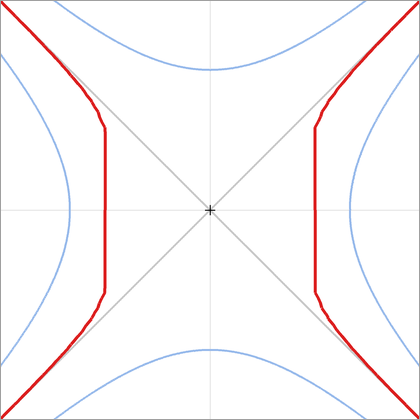
\includegraphics[width=0.2\textwidth]{pictures/report/interp/interp_A1_1_vertex_mid_from_minus.png} &
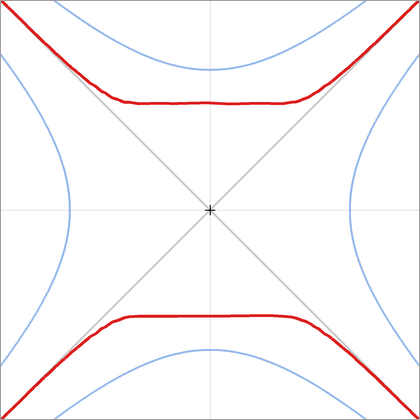
\includegraphics[width=0.2\textwidth]{pictures/report/interp/interp_A1_1_vertex_mid_from_plus.png} &
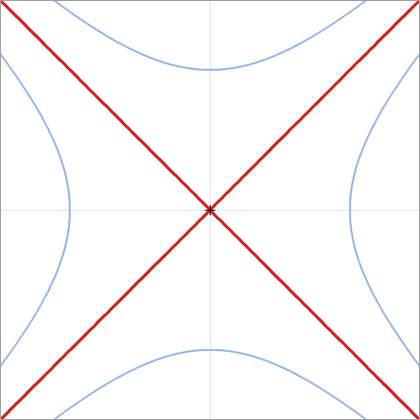
\includegraphics[width=0.2\textwidth]{pictures/report/interp/interp_A1_1_sdf_average.png} &
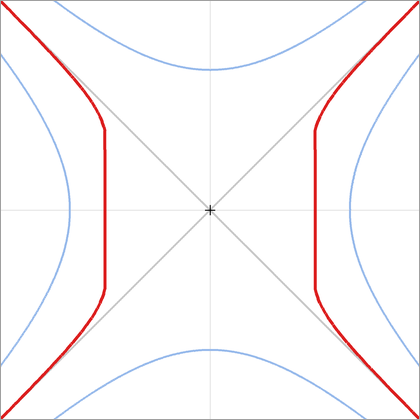
\includegraphics[width=0.2\textwidth]{pictures/report/interp/interp_A1_1_exact_vertex_mid.png} \\
\rotatebox{90}{\scriptsize\ \ \ $x^2+y^2-z^2+xyz$, $G=x$} &
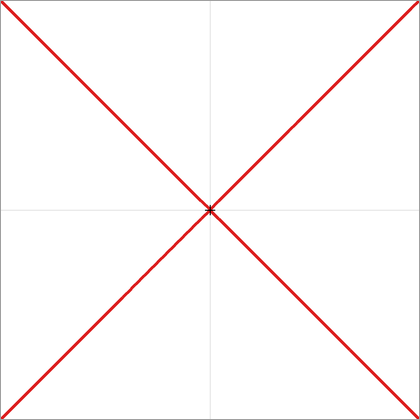
\includegraphics[width=0.2\textwidth]{pictures/report/interp/interp_A1_x_vertex_mid_from_minus.png} &
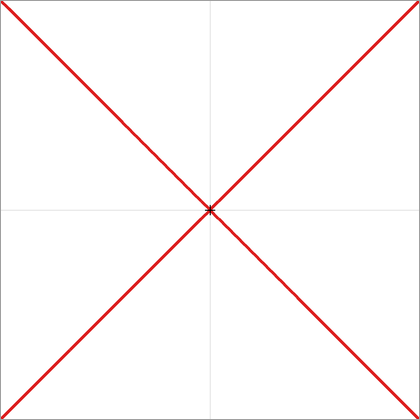
\includegraphics[width=0.2\textwidth]{pictures/report/interp/interp_A1_x_vertex_mid_from_plus.png} &
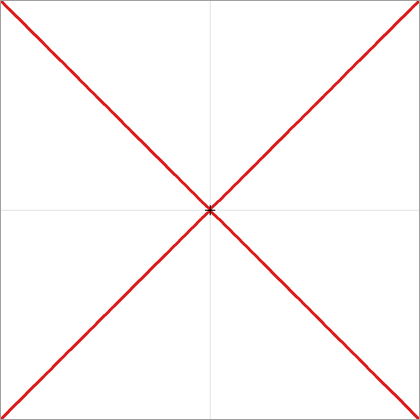
\includegraphics[width=0.2\textwidth]{pictures/report/interp/interp_A1_x_sdf_average.png} &
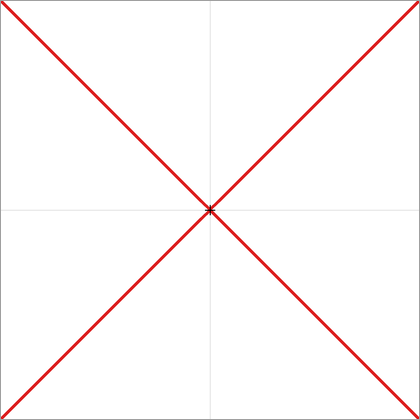
\includegraphics[width=0.2\textwidth]{pictures/report/interp/interp_A1_x_exact_vertex_mid.png} \\
\rotatebox{90}{\scriptsize\ \ \ \ \ \ \ $x^2+y^2+z^3$, $G=x$} &
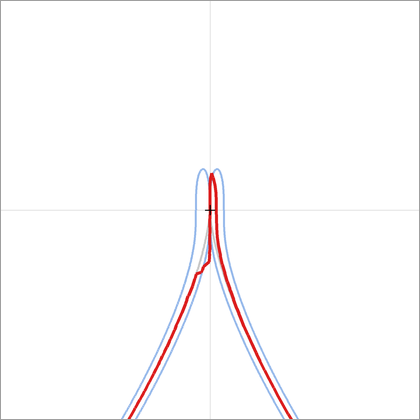
\includegraphics[width=0.2\textwidth]{pictures/report/interp/interp_A2a_x_vertex_mid_from_minus.png} &
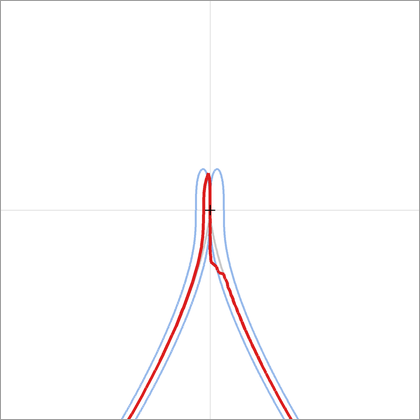
\includegraphics[width=0.2\textwidth]{pictures/report/interp/interp_A2a_x_vertex_mid_from_plus.png} &
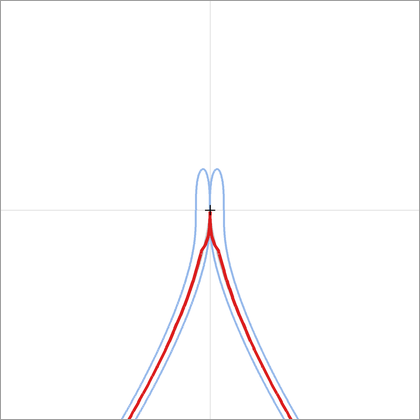
\includegraphics[width=0.2\textwidth]{pictures/report/interp/interp_A2a_x_sdf_average.png} &
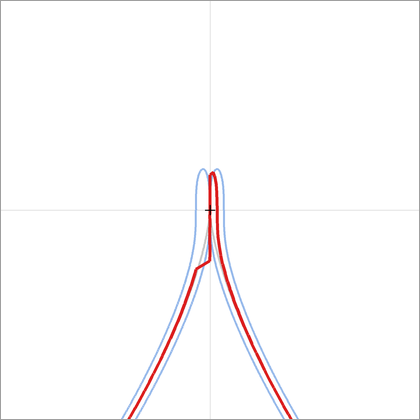
\includegraphics[width=0.2\textwidth]{pictures/report/interp/interp_A2a_x_exact_vertex_mid.png} \\
\rotatebox{90}{\scriptsize\ \ \ \ \ \ \ $x^3+y^3+z^3$, $G=x$} &
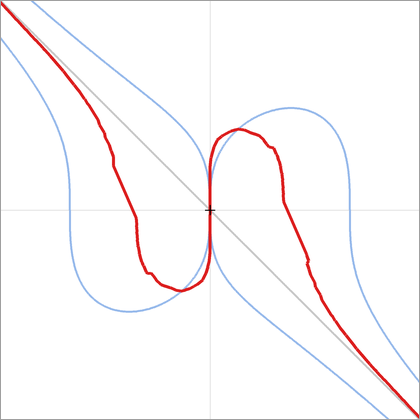
\includegraphics[width=0.2\textwidth]{pictures/report/interp/interp_E6a_x_vertex_mid_from_minus.png} &
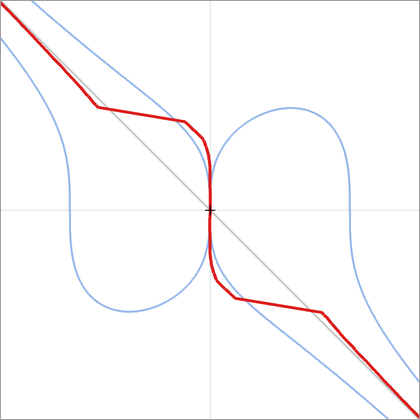
\includegraphics[width=0.2\textwidth]{pictures/report/interp/interp_E6a_x_vertex_mid_from_plus.png} &
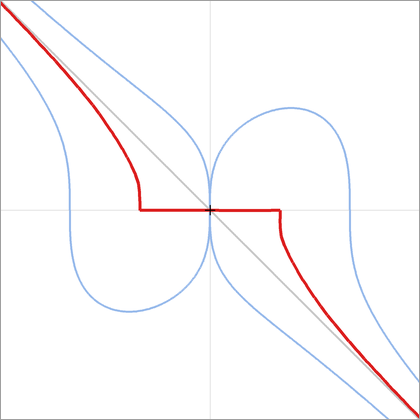
\includegraphics[width=0.2\textwidth]{pictures/report/interp/interp_E6a_x_sdf_average.png} &
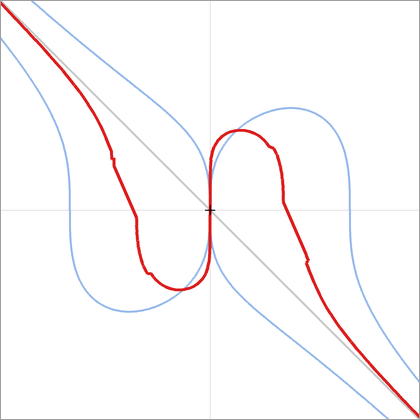
\includegraphics[width=0.2\textwidth]{pictures/report/interp/interp_E6a_x_exact_vertex_mid.png} \\
\end{tabular}
\caption{Slices of the reconstructions of $S_0$ through $P$ for $\varepsilon=0.01$,
$N=128$ (planes $x=0$, $x=0$, $y=0$, $z=0$; window $[-0.15,0.15]^2$). Light blue:
the exact $S_{-\varepsilon}$ and $S_{+\varepsilon}$; grey: the exact $S_0$; red:
the reconstruction. Row 1: the vertex interpolations keep the topology of their
source (one sheet with a waist, two separate sheets) and miss the pinch at $P$; the
SDF interpolation is the cone. Row 2: the deformation is a shift by $\pm k/2$,
which cancels: all reconstructions are the cone. Row 3: the spike is in both
$S_{\pm\varepsilon}$ and stays. Row 4: different shapes on the two sides; no
reconstruction is correct near $P$.}
\label{fig:interp-slices}
\end{figure}

\paragraph{Topology.} Table~\ref{tab:interp-topology} counts, over the $200$ runs at
$N=128$, how often the reconstruction has the same number of components and the
same Euler characteristic in $Q$ as the direct mesh of $F$. The vertex
interpolations agree exactly as often as their source meshes do ($163$ against
$164$ for $S_{-\varepsilon}$, $184$ against $185$ for $S_{+\varepsilon}$): they
inherit the topology of the source, as predicted. Where the topologies differ, it
is the perturbation that changed them, for example $G=1$ on the double point
($S_{-\varepsilon}$ is one sheet with $\chi=0$, $S_0$ two cones with $\chi=2$),
$G=1$ on $x^2+y^3-3yz^2$ (one sheet instead of three) or $G=x+y$ on
$x^3+y^3+z^2+x^2$ (two components instead of one). In addition, the vertex
interpolation folds the mesh near $P$ (flipped triangles) in $40$--$50\%$ of the
runs. The SDF interpolation has the topology of $F$'s mesh in $197$ of the $200$
runs and never folds; it is the only one of the three that can create or remove a
pinch. No reconstruction had holes.

\begin{table}[!ht]
\centering
\small
\begin{tabular}{l c c c}
\toprule
& \makecell{same topology\\as mesh of $F$}
& \makecell{runs with\\flipped triangles}
& \makecell{runs with\\non-manifold edges} \\
\midrule
mesh of $S_{-\varepsilon}$ & 164 & -- & 0 \\
mesh of $S_{+\varepsilon}$ & 185 & -- & 1 \\
vertex interpolation from $S_{-\varepsilon}$ & 163 & 79 & 0 \\
vertex interpolation from $S_{+\varepsilon}$ & 184 & 81 & 1 \\
vertex interpolation (exact) & 163 & 102 & 0 \\
SDF interpolation & 197 & -- & 3 \\
\bottomrule
\end{tabular}
\caption[Interpolation: topology]{Topology of the reconstructions inside $Q$ over the $200$ runs at $N=128$ ($40$ pairs, $5$ values of $\varepsilon$). ``Same topology'': the same number of connected components and the same Euler characteristic as the direct Marching Cubes mesh of $F$.}
\label{tab:interp-topology}
\end{table}

\paragraph{Grid resolution.} The median error at $\varepsilon=10^{-3}$ over the $40$
pairs is
\begin{center}
\small
\begin{tabular}{c c c c c c}
\toprule
$N$ & direct mesh of $F$ & $S_{\pm\varepsilon}$ & vertex (mesh) & vertex (exact) & SDF \\
\midrule
32  & 0.0080 & 0.018 & 0.012 & 0.012 & 0.0084 \\
64  & 0.0041 & 0.021 & 0.015 & 0.012 & 0.0066 \\
128 & 0.0021 & 0.021 & 0.016 & 0.012 & 0.0043 \\
\bottomrule
\end{tabular}
\end{center}
The direct mesh of $F$ improves with the grid. The endpoints and the vertex
interpolations do not: their error is the actual difference between the
interpolated and the singular surface near $P$, which a finer grid only shows more
clearly. The SDF interpolation improves with $N$, but more slowly than the direct
mesh.

Tables~\ref{tab:interp-pairs-1} and ~\ref{tab:interp-pairs-2} lists the error in $Q$ for every pair.
\begin{comment}
\begin{table}[H]
\centering
\footnotesize
\begin{adjustbox}{max width=\textwidth}
\begin{tabular}{l l c c c c c c c c}
\toprule
& & \multicolumn{4}{c}{$\varepsilon=10^{-2}$} & \multicolumn{4}{c}{$\varepsilon=10^{-3}$} \\
\cmidrule(lr){3-6}\cmidrule(lr){7-10}
$F$ & $G$ & $S_{\pm\varepsilon}$ & vertex & SDF & exact & $S_{\pm\varepsilon}$ & vertex & SDF & exact \\
\midrule
$x^2+y^2-z^2+xyz$ & $1$ & 0.1000 & 0.0762 & 0.0013 & 0.0750 & 0.0316 & 0.0247 & 0.0014 & 0.0237 \\
 & $x$ & 0.0063 & 0.0040 & 0.0018 & 0.0046 & 0.0016 & 0.0015 & 0.0013 & 0.0013 \\
 & $x+y$ & 0.0093 & 0.0065 & 0.0024 & 0.0060 & 0.0017 & 0.0016 & 0.0013 & 0.0013 \\
 & $x^2+y^2-z^2$ & 0.0014 & 0.0014 & 0.0014 & 0.0013 & 0.0014 & 0.0014 & 0.0014 & 0.0013 \\
\midrule
$x^2+y^2+z^3$ & $1$ & empty & empty & 0.1102 & 0.1331 & 0.1000 & 0.0948 & 0.0650 & 0.0121 \\
 & $x$ & 0.0269 & 0.0244 & 0.0025 & 0.0256 & 0.0022 & 0.0022 & 0.0024 & 0.0021 \\
 & $x+y$ & 0.0342 & 0.0303 & 0.0025 & 0.0317 & 0.0024 & 0.0024 & 0.0025 & 0.0018 \\
 & $x^2+y^2-z^2$ & 0.0080 & 0.0080 & 0.0112 & 0.0099 & 0.0022 & 0.0021 & 0.0024 & 0.0015 \\
\midrule
$x^2-y^2+z^3$ & $1$ & 0.1000 & 0.0750 & 0.0199 & 0.0753 & 0.0316 & 0.0243 & 0.0076 & 0.0243 \\
 & $x$ & 0.0067 & 0.0067 & 0.0024 & 0.0065 & 0.0017 & 0.0015 & 0.0013 & 0.0016 \\
 & $x+y$ & 0.0075 & 0.0083 & 0.0026 & 0.0082 & 0.0017 & 0.0015 & 0.0012 & 0.0016 \\
 & $x^2+y^2-z^2$ & 0.0024 & 0.0015 & 0.0012 & 0.0009 & 0.0015 & 0.0015 & 0.0011 & 0.0007 \\
\midrule
$x^3+y^3+z^2+x^2$ & $1$ & empty & empty & 0.1126 & 0.1334 & 0.1000 & 0.0948 & 0.0655 & 0.0123 \\
 & $x$ & 0.0269 & 0.0244 & 0.0025 & 0.0255 & 0.0022 & 0.0022 & 0.0024 & 0.0021 \\
 & $x+y$ & 0.1006 & 0.0514 & 0.0709 & 0.0516 & 0.0313 & 0.0158 & 0.0269 & 0.0159 \\
 & $x^2+y^2-z^2$ & 0.0080 & 0.0080 & 0.0112 & 0.0040 & 0.0022 & 0.0022 & 0.0024 & 0.0015 \\
\midrule
$x^2+y^3+z^3$ & $1$ & 0.2418 & 0.2154 & 0.1101 & 0.1828 & 0.1121 & 0.0939 & 0.0649 & 0.0360 \\
 & $x$ & 0.0321 & 0.0294 & 0.0018 & 0.0303 & 0.0018 & 0.0015 & 0.0038 & 0.0025 \\
 & $x+y$ & 0.1053 & 0.0645 & 0.0418 & 0.0642 & 0.0324 & 0.0199 & 0.0159 & 0.0198 \\
 & $x^2+y^2-z^2$ & 0.0056 & 0.0027 & 0.0082 & 0.0048 & 0.0016 & 0.0015 & 0.0036 & 0.0011 \\
\midrule
$x^2+y^3-3yz^2$ & $1$ & 0.2154 & 0.2007 & 0.1102 & 0.0772 & 0.1000 & 0.0945 & 0.0649 & 0.0367 \\
 & $x$ & 0.0155 & 0.0129 & 0.0039 & 0.0137 & 0.0027 & 0.0027 & 0.0041 & 0.0027 \\
 & $x+y$ & 0.0518 & 0.0478 & 0.0519 & 0.0479 & 0.0166 & 0.0165 & 0.0198 & 0.0166 \\
 & $x^2+y^2-z^2$ & 0.0043 & 0.0042 & 0.0095 & 0.0037 & 0.0028 & 0.0028 & 0.0053 & 0.0029 \\
\midrule
$x^3+y^3+z^3$ & $1$ & 0.2520 & 0.1805 & 0.0094 & 0.1804 & 0.1169 & 0.0606 & 0.0043 & 0.0603 \\
 & $x$ & 0.1026 & 0.0668 & 0.0354 & 0.0666 & 0.0315 & 0.0206 & 0.0089 & 0.0208 \\
 & $x+y$ & 0.1379 & 0.0784 & 0.0413 & 0.0784 & 0.0433 & 0.0246 & 0.0119 & 0.0246 \\
 & $x^2+y^2-z^2$ & 0.0080 & 0.0058 & 0.0018 & 0.0076 & 0.0022 & 0.0018 & 0.0018 & 0.0017 \\
\midrule
$x^3+y^3-z^3$ & $1$ & 0.2520 & 0.1805 & 0.0094 & 0.1804 & 0.1169 & 0.0605 & 0.0043 & 0.0605 \\
 & $x$ & 0.1026 & 0.0668 & 0.0354 & 0.0666 & 0.0315 & 0.0206 & 0.0089 & 0.0208 \\
 & $x+y$ & 0.1379 & 0.0784 & 0.0413 & 0.0784 & 0.0433 & 0.0245 & 0.0119 & 0.0246 \\
 & $x^2+y^2-z^2$ & 0.0080 & 0.0058 & 0.0018 & 0.0076 & 0.0022 & 0.0018 & 0.0018 & 0.0017 \\
\midrule
$x^3+y^3+z^3+xyz$ & $1$ & 0.2216 & 0.1478 & 0.0060 & 0.1480 & 0.1028 & 0.0650 & 0.0027 & 0.0652 \\
 & $x$ & 0.0875 & 0.0585 & 0.0346 & 0.0587 & 0.0274 & 0.0178 & 0.0087 & 0.0183 \\
 & $x+y$ & 0.1153 & 0.0670 & 0.0440 & 0.0669 & 0.0359 & 0.0212 & 0.0106 & 0.0211 \\
 & $x^2+y^2-z^2$ & 0.0068 & 0.0050 & 0.0027 & 0.0068 & 0.0027 & 0.0026 & 0.0026 & 0.0026 \\
\midrule
$x^3+2y^3+3z^3+2xyz$ & $1$ & 0.1782 & 0.1331 & 0.0371 & 0.1335 & 0.0828 & 0.0570 & 0.0174 & 0.0574 \\
 & $x$ & 0.0688 & 0.0436 & 0.0279 & 0.0435 & 0.0207 & 0.0136 & 0.0090 & 0.0137 \\
 & $x+y$ & 0.0815 & 0.0480 & 0.0350 & 0.0480 & 0.0255 & 0.0155 & 0.0079 & 0.0151 \\
 & $x^2+y^2-z^2$ & 0.0053 & 0.0042 & 0.0039 & 0.0047 & 0.0032 & 0.0031 & 0.0031 & 0.0027 \\
\bottomrule
\end{tabular}
\end{adjustbox}
\caption[Interpolation: all pairs]{Local Hausdorff distance in $Q$ between the reconstruction and the exact $S_0$, $N=128$. ``$S_{\pm\varepsilon}$'': the worse endpoint mesh; ``vertex'': the worse of the two mesh vertex interpolations; ``exact'': vertex interpolation on the exact surfaces; ``empty'': $S_{+\varepsilon}$ has no part in $Q$ (the tip of the horn moved out of the box). For comparison, the direct mesh of $F$ has the error $0.0014$--$0.0030$.}
\label{tab:interp-pairs}
\end{table}
\end{comment}
\begin{table}[!ht]
\centering
\footnotesize
\setlength{\tabcolsep}{4pt}
\begin{adjustbox}{max width=\textwidth}
\begin{tabular}{l l c c c c c c c c}
\toprule
& & \multicolumn{4}{c}{$\varepsilon=10^{-2}$} & \multicolumn{4}{c}{$\varepsilon=10^{-3}$} \\
\cmidrule(lr){3-6}\cmidrule(lr){7-10}
$F$ & $G$ & $S_{\pm\varepsilon}$ & vertex & SDF & exact & $S_{\pm\varepsilon}$ & vertex & SDF & exact \\
\midrule
$x^2+y^2-z^2+xyz$ & $1$ & 0.1000 & 0.0762 & 0.0013 & 0.0750 & 0.0316 & 0.0247 & 0.0014 & 0.0237 \\
 & $x$ & 0.0063 & 0.0040 & 0.0018 & 0.0046 & 0.0016 & 0.0015 & 0.0013 & 0.0013 \\
 & $x+y$ & 0.0093 & 0.0065 & 0.0024 & 0.0060 & 0.0017 & 0.0016 & 0.0013 & 0.0013 \\
 & $x^2+y^2-z^2$ & 0.0014 & 0.0014 & 0.0014 & 0.0013 & 0.0014 & 0.0014 & 0.0014 & 0.0013 \\
\midrule
$x^2+y^2+z^3$ & $1$ & empty & empty & 0.1102 & 0.1331 & 0.1000 & 0.0948 & 0.0650 & 0.0121 \\
 & $x$ & 0.0269 & 0.0244 & 0.0025 & 0.0256 & 0.0022 & 0.0022 & 0.0024 & 0.0021 \\
 & $x+y$ & 0.0342 & 0.0303 & 0.0025 & 0.0317 & 0.0024 & 0.0024 & 0.0025 & 0.0018 \\
 & $x^2+y^2-z^2$ & 0.0080 & 0.0080 & 0.0112 & 0.0099 & 0.0022 & 0.0021 & 0.0024 & 0.0015 \\
\midrule
$x^2-y^2+z^3$ & $1$ & 0.1000 & 0.0750 & 0.0199 & 0.0753 & 0.0316 & 0.0243 & 0.0076 & 0.0243 \\
 & $x$ & 0.0067 & 0.0067 & 0.0024 & 0.0065 & 0.0017 & 0.0015 & 0.0013 & 0.0016 \\
 & $x+y$ & 0.0075 & 0.0083 & 0.0026 & 0.0082 & 0.0017 & 0.0015 & 0.0012 & 0.0016 \\
 & $x^2+y^2-z^2$ & 0.0024 & 0.0015 & 0.0012 & 0.0009 & 0.0015 & 0.0015 & 0.0011 & 0.0007 \\
\midrule
$x^3+y^3+z^2+x^2$ & $1$ & empty & empty & 0.1126 & 0.1334 & 0.1000 & 0.0948 & 0.0655 & 0.0123 \\
 & $x$ & 0.0269 & 0.0244 & 0.0025 & 0.0255 & 0.0022 & 0.0022 & 0.0024 & 0.0021 \\
 & $x+y$ & 0.1006 & 0.0514 & 0.0709 & 0.0516 & 0.0313 & 0.0158 & 0.0269 & 0.0159 \\
 & $x^2+y^2-z^2$ & 0.0080 & 0.0080 & 0.0112 & 0.0040 & 0.0022 & 0.0022 & 0.0024 & 0.0015 \\
\midrule
$x^2+y^3+z^3$ & $1$ & 0.2418 & 0.2154 & 0.1101 & 0.1828 & 0.1121 & 0.0939 & 0.0649 & 0.0360 \\
 & $x$ & 0.0321 & 0.0294 & 0.0018 & 0.0303 & 0.0018 & 0.0015 & 0.0038 & 0.0025 \\
 & $x+y$ & 0.1053 & 0.0645 & 0.0418 & 0.0642 & 0.0324 & 0.0199 & 0.0159 & 0.0198 \\
 & $x^2+y^2-z^2$ & 0.0056 & 0.0027 & 0.0082 & 0.0048 & 0.0016 & 0.0015 & 0.0036 & 0.0011 \\
\bottomrule
\end{tabular}
\end{adjustbox}
\caption[Interpolation: all pairs (1/2)]{Local Hausdorff distance in $Q$ between the reconstruction and the exact $S_0$, $N=128$. ``$S_{\pm\varepsilon}$'': the worse endpoint mesh; ``vertex'': the worse of the two mesh vertex interpolations; ``exact'': vertex interpolation on the exact surfaces; ``empty'': $S_{+\varepsilon}$ has no part in $Q$. For comparison, the direct mesh of $F$ has an error of $0.0014$--$0.0030$.}
\label{tab:interp-pairs-1}
\end{table}
\begin{table}[!ht]
\centering
\footnotesize
\setlength{\tabcolsep}{4pt}
\begin{adjustbox}{max width=\textwidth}
\begin{tabular}{l l c c c c c c c c}
\toprule
& & \multicolumn{4}{c}{$\varepsilon=10^{-2}$} & \multicolumn{4}{c}{$\varepsilon=10^{-3}$} \\
\cmidrule(lr){3-6}\cmidrule(lr){7-10}
$F$ & $G$ & $S_{\pm\varepsilon}$ & vertex & SDF & exact & $S_{\pm\varepsilon}$ & vertex & SDF & exact \\
\midrule
$x^2+y^3-3yz^2$ & $1$ & 0.2154 & 0.2007 & 0.1102 & 0.0772 & 0.1000 & 0.0945 & 0.0649 & 0.0367 \\
 & $x$ & 0.0155 & 0.0129 & 0.0039 & 0.0137 & 0.0027 & 0.0027 & 0.0041 & 0.0027 \\
 & $x+y$ & 0.0518 & 0.0478 & 0.0519 & 0.0479 & 0.0166 & 0.0165 & 0.0198 & 0.0166 \\
 & $x^2+y^2-z^2$ & 0.0043 & 0.0042 & 0.0095 & 0.0037 & 0.0028 & 0.0028 & 0.0053 & 0.0029 \\
\midrule
$x^3+y^3+z^3$ & $1$ & 0.2520 & 0.1805 & 0.0094 & 0.1804 & 0.1169 & 0.0606 & 0.0043 & 0.0603 \\
 & $x$ & 0.1026 & 0.0668 & 0.0354 & 0.0666 & 0.0315 & 0.0206 & 0.0089 & 0.0208 \\
 & $x+y$ & 0.1379 & 0.0784 & 0.0413 & 0.0784 & 0.0433 & 0.0246 & 0.0119 & 0.0246 \\
 & $x^2+y^2-z^2$ & 0.0080 & 0.0058 & 0.0018 & 0.0076 & 0.0022 & 0.0018 & 0.0018 & 0.0017 \\
\midrule
$x^3+y^3-z^3$ & $1$ & 0.2520 & 0.1805 & 0.0094 & 0.1804 & 0.1169 & 0.0605 & 0.0043 & 0.0605 \\
 & $x$ & 0.1026 & 0.0668 & 0.0354 & 0.0666 & 0.0315 & 0.0206 & 0.0089 & 0.0208 \\
 & $x+y$ & 0.1379 & 0.0784 & 0.0413 & 0.0784 & 0.0433 & 0.0245 & 0.0119 & 0.0246 \\
 & $x^2+y^2-z^2$ & 0.0080 & 0.0058 & 0.0018 & 0.0076 & 0.0022 & 0.0018 & 0.0018 & 0.0017 \\
\midrule
$x^3+y^3+z^3+xyz$ & $1$ & 0.2216 & 0.1478 & 0.0060 & 0.1480 & 0.1028 & 0.0650 & 0.0027 & 0.0652 \\
 & $x$ & 0.0875 & 0.0585 & 0.0346 & 0.0587 & 0.0274 & 0.0178 & 0.0087 & 0.0183 \\
 & $x+y$ & 0.1153 & 0.0670 & 0.0440 & 0.0669 & 0.0359 & 0.0212 & 0.0106 & 0.0211 \\
 & $x^2+y^2-z^2$ & 0.0068 & 0.0050 & 0.0027 & 0.0068 & 0.0027 & 0.0026 & 0.0026 & 0.0026 \\
\midrule
$x^3+2y^3+3z^3+2xyz$ & $1$ & 0.1782 & 0.1331 & 0.0371 & 0.1335 & 0.0828 & 0.0570 & 0.0174 & 0.0574 \\
 & $x$ & 0.0688 & 0.0436 & 0.0279 & 0.0435 & 0.0207 & 0.0136 & 0.0090 & 0.0137 \\
 & $x+y$ & 0.0815 & 0.0480 & 0.0350 & 0.0480 & 0.0255 & 0.0155 & 0.0079 & 0.0151 \\
 & $x^2+y^2-z^2$ & 0.0053 & 0.0042 & 0.0039 & 0.0047 & 0.0032 & 0.0031 & 0.0031 & 0.0027 \\
\bottomrule
\end{tabular}
\end{adjustbox}
\caption[Interpolation: all pairs (2/2)]{Local Hausdorff distance in $Q$ between the reconstruction and the exact $S_0$, $N=128$. The columns have the same meaning as in Table~\ref{tab:interp-pairs-1}.}
\label{tab:interp-pairs-2}
\end{table}

\subsection{Conclusion of the interpolation experiment}

Linear interpolation between $S_{-\varepsilon}$ and $S_{+\varepsilon}$ reconstructs
$S_0$ to \emph{second order} away from the singular point: the first-order changes
of the two sides cancel, and already for $\varepsilon=10^{-3}$ the error there is
that of a direct mesh. Near the singular point it does not: the two sides of the
deformation are different shapes of size $\lambda(\varepsilon)$, nothing cancels,
and the error decreases with the same rate $\varepsilon^\alpha$ as for
$S_{\pm\varepsilon}$ alone. Vertex interpolation also cannot change the topology,
so it never recreates the singular point when the perturbation removed it, and it
often folds the mesh near $P$. Interpolating distance fields can recreate the
singular point, but reliably only when the deformation is symmetric with respect to
$S_0$. Interpolating the implicit functions is exact, but returns the original
problem of meshing $\{F=0\}$.

% =============================================================================
\section{A Singularity-Aware Extraction: the Weighted Cone Patch}
\label{sec:r-cone}
% =============================================================================

Section~\ref{sec:r-interp} leaves two facts. First, averaging the implicit values
reconstructs $F$ exactly, so no reconstruction from $S_{\pm\varepsilon}$ can be better
than a good extraction of $S_0$ itself. Second, all defects are confined to a small
neighbourhood of $P$, and the structure of $S_0$ there is known from the scaling of
Section~\ref{sec:r-scaling}. This section uses the second fact to change the
extraction near $P$, and then returns to $S_{\pm\varepsilon}$.

\subsection{The idea}
\label{sec:r-cone-idea}

Let $F_0$ be the weighted principal part of $F$ at $P=0$, with weights
$w=(w_x,w_y,w_z)$ (Section~\ref{sec:r-scaling}), and for $0<t\le1$ let
\[
\Phi_t(x,y,z)=\big(t^{w_x}x,\ t^{w_y}y,\ t^{w_z}z\big).
\]
Then $F_0(\Phi_t(p))=t\,F_0(p)$, so $\Phi_t$ maps the surface $\{F_0=0\}$ into itself
and moves every point of it towards $P$. For the cubic cones ($w=(\tfrac13,\tfrac13,\tfrac13)$)
$\Phi_t$ is the ordinary scaling by $t^{1/3}$; for the horn $x^2+y^2+z^3$ the orbits
$t\mapsto(t^{1/2}x,t^{1/2}y,t^{1/3}z)$ follow the horn into its tip. Two properties
follow.
\begin{enumerate}
    \item Every orbit $\{\Phi_t(p):0<t\le1\}$ enters the box $B=P+[-r,r]^3$ exactly
          once, because each coordinate $|t^{w_i}p_i|$ decreases with $t$.
    \item Hence $\{F_0=0\}\cap B$ is the union of the orbits through the curve
          $L=\{F_0=0\}\cap\partial B$: it is a cone over $L$ with apex $P$, built from
          scaled copies of $L$.
\end{enumerate}
$F$ differs from $F_0$ by terms of weighted degree larger than $1$, which are small
near $P$, so for $F$ the same holds up to a small correction that Newton's method
removes. Topologically it holds exactly: by the conic structure theorem
\cite{milnor1968singular}, for a small enough box $S_0\cap B$ is homeomorphic to the
cone over its link $S_0\cap\partial B$. A cone is contractible, so a correct mesh of
$S_0\cap B$ is connected and has Euler characteristic $\chi=1$, however many components
the link has.

\subsection{The algorithm}
\label{sec:r-cone-algorithm}

The input is the grid of $F$ (equivalently the average of the grids of $H_{-\varepsilon}$
and $H_{+\varepsilon}$), the singular point $P$, the weights $w$ (computed from the
Taylor coefficients of $F$ at $P$ up to degree $3$, by the same function that predicts
$\alpha$) and the box radius $r=4h$.
\begin{enumerate}
    \item Extract $S_0$ by Marching Cubes.
    \item Remove every triangle with a corner inside $B$.
    \item The boundary edges of the remaining mesh next to $\partial B$ form closed
          loops, the discrete link. Move their vertices onto $S_0$ by Newton's
          method.
    \item For $j=1,2,\dots$ place the ring $\Phi_{t_j}(\text{loop})$, $t_j=\rho^j$,
          move each of its vertices onto $S_0$ by Newton's method, and connect it to
          the previous ring by two triangles per loop edge. $\rho$ is chosen so that
          the slowest coordinate shrinks by the factor $1-h/r$ per ring: the first
          ring lies inside $B$, and the rings are similar copies of the loop whose
          spacing matches the length of its edges.
    \item When a ring is smaller than $h/20$, connect it to $P$.
\end{enumerate}
The new triangles have the orientation of the loop, so the mesh stays consistently
oriented. A link with several components (the two nappes of the double cone, the
three pieces of $x^2+y^3-3yz^2$) gives several loops; each gets its own cone, and all
of them share the vertex $P$.

\paragraph{Where the method applies.} The method needs the point $P$ and an isolated
singular point whose principal part is weighted homogeneous and nondegenerate, i.e.\
$F=F_0+(\text{terms of weighted degree}>1)$ with $\nabla F_0\neq0$ away from $P$ (a
\emph{semi-quasihomogeneous} singularity \cite{arnold2012singularities}). The program
checks this: it finds the weights from the Taylor coefficients up to degree $3$ and
tests the nondegeneracy of $F_0$ numerically; otherwise it keeps the Marching Cubes
mesh and says so. All ten surfaces of this report belong to this class. So do all simple
singularities $A_k$, $D_k$, $E_6$, $E_7$, $E_8$ \cite{arnold2012singularities}, but the
program reads only the Taylor coefficients up to degree $3$ and therefore finds the
weights only when the principal part has degree at most $3$ ($A_1$, $A_2$, $D_4$ and
the cubic cones); $x^2+y^2+z^4$ ($A_3$), for example, would need the $4$-jet. Not
covered at all are non-isolated singularities (curves of singular points) and
several singular points closer to each other than $r$.

\subsection{Using only $S_{-\varepsilon}$ and $S_{+\varepsilon}$: the hybrid}
\label{sec:r-cone-hybrid}

The same patch can be put on the vertex interpolation of Section~\ref{sec:r-interp},
without using $F$: outside $B$ the mesh is the vertex interpolation of
$S_{-\varepsilon}$ and $S_{+\varepsilon}$, and inside $B$ the rings are scaled copies of
its boundary loop, not projected. Only $P$ and the weights are needed. Since the two
sides differ near $P$ on the scale of the deformation, the box must contain that
region: $r=\max(4h,\,2\varepsilon^{\alpha})$, with $\alpha$ the lower end of the
predicted rate (Section~\ref{sec:r-scaling}), and at most $0.24$. Outside $B$ the
interpolation is of second order in $\varepsilon$
(Section~\ref{sec:r-interp-theory}); inside, the error is that of the loop, scaled
down.

\subsection{Correspondence along the gradient of $F$}
\label{sec:r-cone-normal}

The second open question of Section~\ref{sec:r-interp} was the correspondence. The
closest point was used because two meshes have no common numbering. A
correspondence that follows the derivation of Section~\ref{sec:r-interp-theory}
exactly is the gradient line of $F$: a point $a$ of $S_{-\varepsilon}$ is paired with
the point $a+s\,n$ of $S_{+\varepsilon}$, $n=\nabla F(a)/\|\nabla F(a)\|$, where $s$ is
found by Newton's method on $H_{+\varepsilon}(a+sn)=0$, and $a$ is moved to
$a+\tfrac s2n$. Where $\nabla F$ vanishes or the line does not reach
$S_{+\varepsilon}$ nearby (more than three times the closest-point distance plus two
cells away), the closest point is used instead.

\subsection{Results}
\label{sec:r-cone-results}

The three new reconstructions were added to the experiment of
Section~\ref{sec:r-interp-setup}: the same $40$ pairs, five values of $\varepsilon$
and three grids, measured against the exact $S_0$ in the same way.

\paragraph{The singular cone patch against Marching Cubes.} The cone patch uses only
$F$, so it does not depend on $G$ or $\varepsilon$. Table~\ref{tab:cone-vs-mc}
compares it with the direct Marching Cubes mesh of $F$ for every surface. Near $P$
the error is smaller on every surface and at every resolution; at $N=128$ the median
over the surfaces drops from $0.0021$ to $0.00055$, a factor of about $4$, and for the
double cone and the Fermat cones by a factor of $7$. Away from $P$ both meshes are the
same ($0.00031$). The topology is correct (one component, $\chi=1$) in all $600$
runs, while Marching Cubes of $F$ is wrong in every run on exactly two surfaces: on
the double cone the two nappes do not touch at $P$ ($2$ components, $\chi=2$), and
on $x^2+y^3-3yz^2$ the three pieces stay separate ($3$ components, $\chi=3$). On
these two surfaces the patch has two and three loops, one per component of the
link, and joins them at $P$.

Figure~\ref{fig:cone-zoom} shows the difference on the grid scale. For the double
cone, Marching Cubes leaves small steps next to $P$ and does not join the lines; the
patch crosses exactly at $P$. For the horn, Marching Cubes follows the tip only
roughly and stops short of it, because the tip is thinner than a cell; the patch
follows it into $P$. This is why the box radius depends on the weights: for the horn
($w=(\tfrac12,\tfrac12,\tfrac13)$) the tip is thinner than two cells up to the distance
$(2h)^{2/3}\approx0.054$ from $P$ at $N=128$, so the box must reach that far (with the
fixed radius $4h=0.025$ the error near $P$ was still $0.0018$). For equal weights
the radius stays $4h$.

The error near $P$ does not decrease regularly with $h$ (the median order between
$N=64$ and $N=128$ is $0.8$ against $1.0$ for Marching Cubes): it is now made of the
Marching Cubes triangles just outside the box and of the long thin triangles of the
rings, and the box radius changes with $h$. It stays below that of Marching Cubes on
the same grid in every case.

\begin{table}[!ht]
\centering
\small
\begin{adjustbox}{max width=\textwidth}
\begin{tabular}{l l c c c c c c c c c}
\toprule
& & \multicolumn{2}{c}{$N=32$} & \multicolumn{2}{c}{$N=64$} & \multicolumn{2}{c}{$N=128$} & \multicolumn{2}{c}{components$/\chi$} & \\
\cmidrule(lr){3-4}\cmidrule(lr){5-6}\cmidrule(lr){7-8}\cmidrule(lr){9-10}
type & $F$ & MC & patch & MC & patch & MC & patch & MC & patch & loops \\
\midrule
$A_1$ & $x^2+y^2-z^2+xyz$ & 0.0058 & 0.00041 & 0.0029 & 0.00031 & 0.0014 & 0.00021 & 2/2 & 1/1 & 2 \\
$A_2$ & $x^2+y^2+z^3$ & 0.0073 & 0.00062 & 0.0041 & 0.00037 & 0.0021 & 0.00055 & 1/1 & 1/1 & 1 \\
$A_2$ & $x^2-y^2+z^3$ & 0.0059 & 0.00032 & 0.0029 & 0.00032 & 0.0015 & 0.00028 & 1/1 & 1/1 & 1 \\
$A_2$ & $x^3+y^3+z^2+x^2$ & 0.0074 & 0.00061 & 0.0041 & 0.00039 & 0.0021 & 0.00055 & 1/1 & 1/1 & 1 \\
$D_4$ & $x^2+y^3+z^3$ & 0.0061 & 0.0019 & 0.0031 & 0.00084 & 0.0015 & 0.00074 & 1/1 & 1/1 & 1 \\
$D_4$ & $x^2+y^3-3yz^2$ & 0.0109 & 0.0021 & 0.0054 & 0.0042 & 0.0027 & 0.00087 & 3/3 & 1/1 & 3 \\
$\tilde E_6$ & $x^3+y^3+z^3$ & 0.0075 & 0.00062 & 0.0037 & 0.00051 & 0.0019 & 0.00028 & 1/1 & 1/1 & 1 \\
$\tilde E_6$ & $x^3+y^3-z^3$ & 0.0075 & 0.00062 & 0.0037 & 0.00051 & 0.0019 & 0.00028 & 1/1 & 1/1 & 1 \\
$\tilde E_6$ & $x^3+y^3+z^3+xyz$ & 0.0107 & 0.0016 & 0.0053 & 0.0012 & 0.0027 & 0.00058 & 1/1 & 1/1 & 1 \\
$\tilde E_6$ & $x^3+2y^3+3z^3+2xyz$ & 0.0122 & 0.0015 & 0.0061 & 0.0012 & 0.0030 & 0.00068 & 1/1 & 1/1 & 1 \\
\bottomrule
\end{tabular}
\end{adjustbox}
\caption[Cone patch against Marching Cubes]{Local Hausdorff distance to the exact
$S_0$ near $P$ ($\|p\|_\infty<0.06$) of the direct Marching Cubes mesh of $F$ (MC)
and of the singular cone patch, and the topology inside $Q$ (number of components and
Euler characteristic; correct is $1/1$). ``Loops'': components of the link found by
the patch.}
\label{tab:cone-vs-mc}
\end{table}

\begin{figure}[!ht]
\centering
\setlength{\tabcolsep}{2pt}
\begin{tabular}{c c c c}
MC of $F$ & cone patch & MC of $F$ & cone patch \\
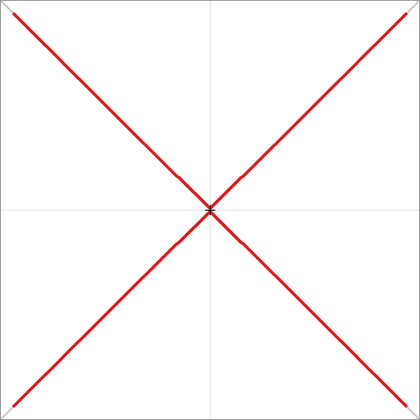
\includegraphics[width=0.22\textwidth]{pictures/report/interp/interp_A1_1_direct_S0_zoom.png} &
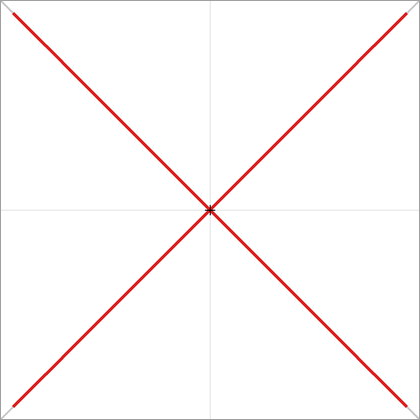
\includegraphics[width=0.22\textwidth]{pictures/report/interp/interp_A1_1_singular_cone_zoom.png} &
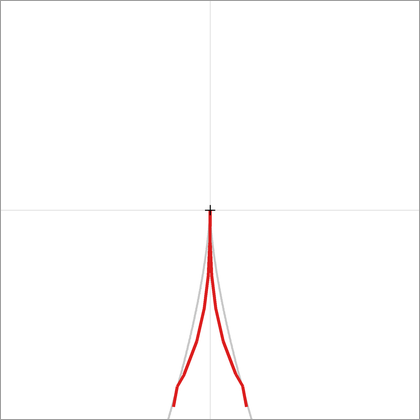
\includegraphics[width=0.22\textwidth]{pictures/report/interp/interp_A2a_x_direct_S0_zoom.png} &
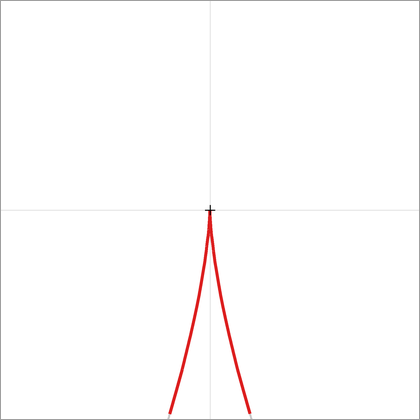
\includegraphics[width=0.22\textwidth]{pictures/report/interp/interp_A2a_x_singular_cone_zoom.png} \\
\multicolumn{2}{c}{\small $x^2+y^2-z^2+xyz$, plane $x=0$} & \multicolumn{2}{c}{\small $x^2+y^2+z^3$, plane $y=0$}
\end{tabular}
\caption{Close-ups of $S_0$ around $P$ (window $[-0.04,0.04]^2$, about $13$ cells at
$N=128$). Grey: the exact $S_0$; red: the mesh.}
\label{fig:cone-zoom}
\end{figure}

\paragraph{All reconstructions together.} Table~\ref{tab:cone-median} extends
Table~\ref{tab:interp-median} by the three new methods.
\begin{itemize}
    \item The \emph{hybrid} (interpolation of $S_{\pm\varepsilon}$ away from $P$, cone
          patch near $P$, no use of $F$) is the only reconstruction from
          $S_{\pm\varepsilon}$ whose error near $P$ does not grow with $\varepsilon$
          like $\varepsilon^\alpha$: from $\varepsilon=10^{-2.5}$ on it is
          $0.0004$--$0.0007$, against $0.0067$--$0.027$ for the vertex
          interpolation, and below the direct mesh of $F$. At $\varepsilon=10^{-2}$
          the deformation reaches across the whole box $Q$, the box of the patch
          ($0.24$) is larger than $Q$, and the error comes from the loop, which lies
          where the interpolation is still poor ($0.0038$ near $P$, $0.013$ away).
          It is within twice the error of the direct mesh in $19$, $33$ and $40$ of
          the $40$ pairs for $\varepsilon=10^{-2},10^{-3},10^{-4}$ (the vertex
          interpolation: $6$, $19$, $23$), and has the correct topology in $599$ of
          the $600$ runs.
    \item The \emph{gradient-line correspondence} improves the vertex interpolation
          away from $P$, most at $\varepsilon=10^{-2}$ ($0.0083$ against $0.037$),
          because it follows the normal expansion of
          Section~\ref{sec:r-interp-theory} instead of approximating it; over the
          $200$ runs at $N=128$ it is better than the closest point in $45$ and worse
          in $8$. Near $P$ it does not help (the same rate as the endpoints), and it
          folds \emph{more} often ($138$ of $200$ runs, against $102$ for the exact
          vertex interpolation): close to $P$ the gradient of $F$ is small and changes
          direction quickly, neighbouring vertices follow very different lines, and
          where the line misses $S_{+\varepsilon}$ the closest point is used instead.
          The folding of the vertex interpolation is a property of the region near
          $P$, not of the choice of correspondence.
\end{itemize}

\begin{table}[!ht]
\centering
\small
\begin{adjustbox}{max width=\textwidth}
\begin{tabular}{l c c c c c c c c c c}
\toprule
& \multicolumn{5}{c}{near $P$} & \multicolumn{5}{c}{away from $P$} \\
\cmidrule(lr){2-6}\cmidrule(lr){7-11}
$\varepsilon$ & $10^{-2}$ & $10^{-2.5}$ & $10^{-3}$ & $10^{-3.5}$ & $10^{-4}$ & $10^{-2}$ & $10^{-2.5}$ & $10^{-3}$ & $10^{-3.5}$ & $10^{-4}$ \\
\midrule
direct mesh of $F$ & 0.0021 & 0.0021 & 0.0021 & 0.0021 & 0.0021 & 0.0003 & 0.0003 & 0.0003 & 0.0003 & 0.0003 \\
vertex interpolation (exact) & 0.048 & 0.023 & 0.012 & 0.0067 & 0.0037 & 0.037 & 0.0022 & 0.0005 & 0.0003 & 0.0003 \\
vertex interp.\ along $\nabla F$ & 0.032 & 0.019 & 0.011 & 0.0064 & 0.0033 & 0.0083 & 0.0013 & 0.0004 & 0.0003 & 0.0003 \\
SDF interpolation & 0.0095 & 0.0064 & 0.0043 & 0.0038 & 0.0026 & 0.0060 & 0.0018 & 0.0007 & 0.0007 & 0.0004 \\
hybrid (interp.\ + cone patch) & 0.0038 & 0.0006 & 0.0007 & 0.0004 & 0.0004 & 0.013 & 0.0007 & 0.0005 & 0.0003 & 0.0003 \\
singular cone patch & 0.0006 & 0.0006 & 0.0006 & 0.0006 & 0.0006 & 0.0003 & 0.0003 & 0.0003 & 0.0003 & 0.0003 \\
\bottomrule
\end{tabular}
\end{adjustbox}
\caption[Reconstructions including the cone patch: median errors]{As
Table~\ref{tab:interp-median} ($N=128$, median over the $40$ pairs), with the
gradient-line correspondence, the hybrid and the singular cone patch.}
\label{tab:cone-median}
\end{table}

\begin{table}[!ht]
\centering
\small
\begin{tabular}{l c c}
\toprule
& \makecell{correct topology\\(1 component, $\chi=1$)} & \makecell{runs with\\flipped triangles} \\
\midrule
direct mesh of $F$ & 160 & -- \\
meshes of $S_{-\varepsilon}$ / $S_{+\varepsilon}$ & 143 / 151 & -- \\
vertex interpolation (mesh, from $S_{-\varepsilon}$) & 142 & 79 \\
vertex interpolation (exact) & 142 & 102 \\
vertex interpolation along $\nabla F$ & 139 & 138 \\
SDF interpolation & 157 & -- \\
hybrid (interpolation + cone patch) & 200 & -- \\
singular cone patch & 200 & -- \\
\bottomrule
\end{tabular}
\caption[Topology against the cone over the link]{Topology inside $Q$ over the $200$
runs at $N=128$, compared with the true topology of $S_0\cap Q$ (a cone, hence one
component and $\chi=1$), not with the mesh of $F$ as in Table~\ref{tab:interp-topology}.}
\label{tab:cone-topology}
\end{table}

\begin{figure}[!ht]
\centering
\setlength{\tabcolsep}{2pt}
\begin{tabular}{l c c c}
& vertex (exact) & along $\nabla F$ & hybrid \\
\rotatebox{90}{\scriptsize\ \ \ $x^2+y^2-z^2+xyz$, $G=1$} &
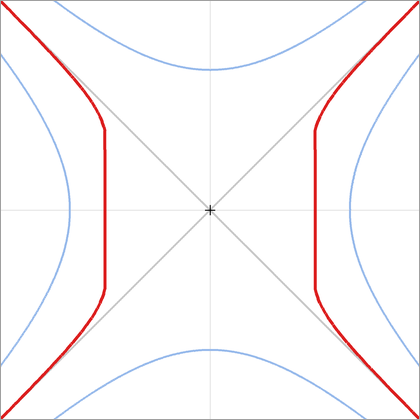
\includegraphics[width=0.24\textwidth]{pictures/report/interp/interp_A1_1_exact_vertex_mid.png} &
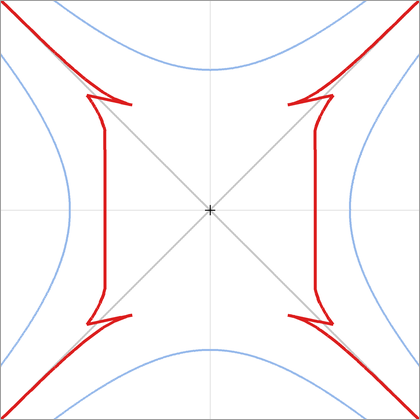
\includegraphics[width=0.24\textwidth]{pictures/report/interp/interp_A1_1_normal_mid.png} &
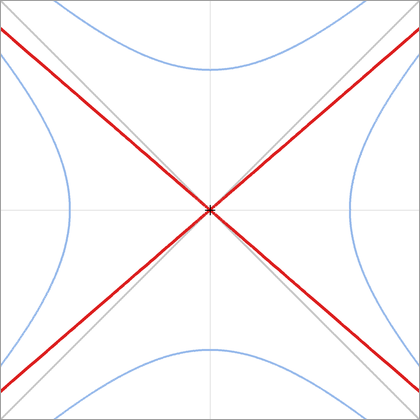
\includegraphics[width=0.24\textwidth]{pictures/report/interp/interp_A1_1_hybrid_cone.png} \\
\rotatebox{90}{\scriptsize\ \ \ \ \ \ \ $x^3+y^3+z^3$, $G=x$} &
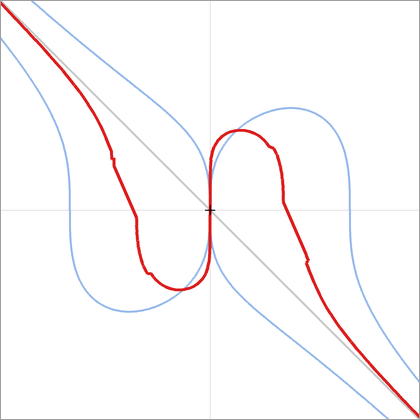
\includegraphics[width=0.24\textwidth]{pictures/report/interp/interp_E6a_x_exact_vertex_mid.png} &
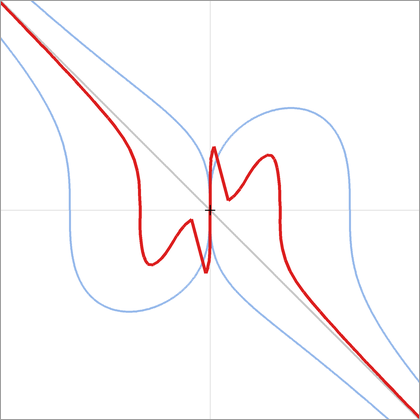
\includegraphics[width=0.24\textwidth]{pictures/report/interp/interp_E6a_x_normal_mid.png} &
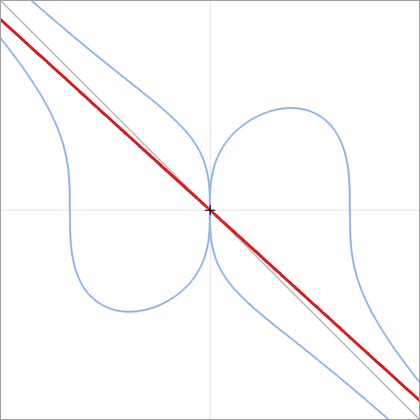
\includegraphics[width=0.24\textwidth]{pictures/report/interp/interp_E6a_x_hybrid_cone.png} \\
\end{tabular}
\caption{Reconstructions from $S_{\pm\varepsilon}$, $\varepsilon=0.01$, $N=128$, as in
Figure~\ref{fig:interp-slices}. The hybrid passes through $P$ and has the shape of
$S_0$ even where the two sides are very different.}
\label{fig:cone-slices}
\end{figure}

\subsection{Conclusion}

The weighted cone patch is a voxel method that models the neighbourhood of an
isolated singular point faithfully: Marching Cubes away from $P$, and near $P$ the
surface rebuilt from its own boundary curve with the scaling that the singularity
itself defines. It gives the topology of the cone over the link in every run, puts
$P$ into the mesh as a vertex, and reduces the error near $P$ by a factor of about $4$
(up to $7$). It applies to isolated singular points with a nondegenerate weighted
homogeneous principal part. The same patch completes the linear interpolation of
$S_{-\varepsilon}$ and $S_{+\varepsilon}$: the interpolation is used where it is of
second order, away from $P$, and the patch replaces it where it cannot work.

% =============================================================================
\section{Conclusions}
\label{sec:r-conclusions}
% =============================================================================

\begin{enumerate}
    \item \textbf{The rate is decided by the type and by the order of $G$.} For the
          cubic cones it is exactly $1/(3-m)$; for the other types it lies in the
          predicted range, and which end appears depends on the sign of $k$ and on
          the real shape (definite or saddle, one or three lines).
    \item \textbf{What happens at $P$ is decided by $G(P)$ and $\nabla G(P)$}, with
          no exception in $144$ pairs.
    \item \textbf{Inessential perturbations mostly move the surface.} Their real
          effect comes at second order and can still be visible: the spike of the
          horn cusp, the moved cusp of the saddle cusp.
    \item \textbf{New singular points are rare and predictable.} They appear only
          for special directions of $G$ (balance condition, three real lines) or for
          quadratic $G$ with indefinite signs; the total multiplicities of the computed stationary
            points agree with the corresponding Milnor numbers.
            However, identifying individual singular points still
            depends on the numerical grouping and zero-level tolerances.
    \item \textbf{Marching Cubes loses exactly what matters near a singular point}:
          thin features and singular points between grid nodes. This is what a
          singularity-aware extraction method has to fix.
    \item \textbf{Linear interpolation between $S_{-\varepsilon}$ and
          $S_{+\varepsilon}$ reconstructs $S_0$ only away from $P$.} There the
          first-order changes cancel and the error is $O(\varepsilon^2)$; near
          $P$ the error decreases with the same rate $\varepsilon^\alpha$ as for
          $S_{\pm\varepsilon}$, vertex interpolation keeps the topology of its
          source, and distance-field interpolation recovers the singular point only
          for symmetric deformations (Section~\ref{sec:r-interp}). Averaging the
          implicit values is exact but gives back the Marching Cubes mesh of $F$.
    \item \textbf{The neighbourhood of $P$ can be extracted faithfully by using its
          weighted scaling.} The weighted cone patch replaces the Marching Cubes
          mesh inside a small box around $P$ by scaled copies of its own boundary
          loop, projected onto $S_0$ (Section~\ref{sec:r-cone}). It has the correct
          topology (a cone over the link) in all $600$ runs, where Marching Cubes
          of $F$ is wrong for the double cone and the three-line $D_4$ point, and
          it reduces the error near $P$ by a factor of about $4$ (median, up to $7$).
          It works for isolated singular points with a nondegenerate weighted
          homogeneous principal part, the class of all ten tested surfaces. Built on
          the vertex interpolation instead of on $F$, the same patch makes the
          interpolation of $S_{-\varepsilon}$ and $S_{+\varepsilon}$ accurate near $P$
          as well.
\end{enumerate}

% =============================================================================
\section{Future Work}
\label{sec:future-work}
% =============================================================================

The experiments presented in this report analyse how singular
surfaces change under polynomial perturbations and how quickly
the perturbed surfaces approach the original singular surface, whether $S_0$ can be
reconstructed by linear interpolation (Section~\ref{sec:r-interp}), and how the
neighbourhood of the singular point can be extracted faithfully
(Section~\ref{sec:r-cone}). Two directions will be investigated in further work.

\paragraph{Extending the cone patch.} The weighted cone patch of
Section~\ref{sec:r-cone} resolves the neighbourhood of one known isolated singular
point with a principal part of degree at most $3$. Four extensions follow.
\begin{itemize}
    \item \emph{Finding $P$.} The stationary-point search of
          Section~\ref{sec:r-method} already finds the singular points of $S_0$;
          the patch can then be applied at each of them, with boxes that do not
          overlap.
    \item \emph{Higher principal parts.} Reading the Taylor coefficients beyond
          degree $3$ would cover $A_k$ for $k\ge3$, $D_k$ for $k\ge5$ and $E_6$,
          $E_7$, $E_8$, which are all weighted homogeneous.
    \item \emph{Triangle shape.} For unequal weights the rings shrink faster
          across the horn than along it, and the triangles near $P$ become long and
          thin. Fewer vertices on the smaller rings would keep them well shaped.
    \item \emph{Non-isolated singularities.} Along a curve of singular points
          (for example the Whitney umbrella $x^2-y^2z$) the conic structure holds
          in the planes transversal to the curve; a patch shaped like a tube
          around the curve is a natural generalisation.
\end{itemize}

\paragraph{Perturbation directions based on the Tjurina algebra.}
The perturbations used in the current experiments were selected
from a predefined set of polynomial expressions. In further
work, the Tjurina algebra will be used to select perturbation
directions systematically.

For each singularity, a basis of the Tjurina algebra will be
computed. The basis elements will then be used individually
as perturbations $G$, together with selected linear
combinations of these elements. Perturbations whose classes
in the Tjurina algebra are zero will also be included as
controls.

This approach will allow us to investigate how independent
deformation directions influence the convergence rate,
the movement and creation of singular points, and the
possibility of reconstructing the original singular surface.

\appendix

% =============================================================================
\section{The Software (for My Own Reference)}
\label{sec:r-software}
% =============================================================================

\paragraph{Where everything is.} The project is a C++17 program with a header-only
library and an interactive viewer:
\begin{itemize}
    \item \texttt{src/core}: parsing and evaluation of expressions (also with automatic
          differentiation), Marching Cubes (\texttt{Isosurface.h}), grid slices and
          snapshots (\texttt{IsosurfaceSlices.h}, \texttt{SliceSnapshot.h}).
    \item \texttt{src/analysis}: the measurements of this report:
          \texttt{ExactDistance.h} (distances on the exact surfaces),
          \texttt{StationaryPoints.h} (numerically computed stationary points and multiplicity checks),
          \texttt{LocalAlgebra.h} (Milnor/Tjurina numbers, essential part),
          \texttt{DirectionSweep.h}, \texttt{ConvergenceClassifier.h} (rates,
          confidence intervals, the classification), \texttt{FamilyAnalysis.h}
          (runs everything for one pair and writes the CSV files),
          \texttt{Reconstruction.h} (all reconstructions of $S_0$ of
          Sections~\ref{sec:r-interp} and~\ref{sec:r-cone}, including the cone
          patch).
    \item \texttt{src/app}: the viewer (PMP library and ImGui).
    \item \texttt{tests}: automated tests (14, all passing) and command-line tools.
\end{itemize}

\paragraph{Reproducing the data.} After building with CMake,
\texttt{./build/isosurface\_thesis\_experiments experiments\_thesis} recomputes all
$144$ pairs in about $17$ minutes. The output is one folder per surface,
resolution and perturbation, with the CSV files
\texttt{exact\_geometry.csv} (distances per $k$), \texttt{stationary\_points\_certified.csv}
(all stationary points per $k$), \texttt{local\_algebra.csv},
\texttt{convergence\_classification.csv}; plus \texttt{classification\_all.csv} with one
row per pair and side, from which all tables of this report are generated.
\texttt{isosurface\_direction\_sweep} draws the direction map for one $F$, and
\texttt{isosurface\_convergence\_classification} classifies a list of $G$ for one $F$.

\paragraph{The interpolation experiment.}
\texttt{./build/isosurface\_interpolation\_experiments interpolation\_results}
(source \texttt{tests/interpolation\_experiments.cpp}) runs the $600$ runs of
Sections~\ref{sec:r-interp} and~\ref{sec:r-cone} in about $7$ minutes and writes
\texttt{interpolation\_results/interpolation\_all.csv}, one row per pair, $\varepsilon$,
grid and method; with \texttt{--slices} it writes the slices of
Figure~\ref{fig:interp-slices}. \texttt{Thesis\_01/scripts/interpolation\_tables.py}
computes the tables and the plot data (\texttt{data/interp\_*.dat}),
\texttt{Thesis\_01/scripts/interpolation\_slices.py} draws the slice pictures, and
\texttt{Thesis\_01/scripts/exact\_slices.py} the exact slices of
Section~\ref{sec:r-surfaces}.

\paragraph{In the viewer.} Under the $k$-sweep, \emph{Classify convergence} runs the
same analysis for the current $F+kG$ and shows the rates, the singular points and the
essential part. The panel \emph{Reconstruct S0 from S-eps and S+eps} builds
$S_{-\varepsilon}$ and $S_{+\varepsilon}$ for the current family and a chosen
$\varepsilon$, reconstructs $S_0$ near the point $P$ with any of the eight methods of
Sections~\ref{sec:r-interp} and~\ref{sec:r-cone}, shows the result in place of the
surface with $S_{\pm\varepsilon}$ as wireframes, and reports its topology and vertex
error near $P$ next to those of the direct Marching Cubes mesh of $F$. The slice gallery's \emph{Create snapshot} saves an SVG and a CSV of a
node window; it now warns when a selected slice contains no part of the surface in
the window, which is how the empty snapshots of the previous report version
happened.

\paragraph{Figures of this report.} The snapshots in \texttt{pictures/report} were
made with the same snapshot code as the viewer and converted to PNG; the exact
slices in \texttt{pictures/report/exact} and the maps in \texttt{data} were drawn
directly from the polynomials and from the CSV files.

\bibliographystyle{alpha}
\bibliography{bibliography}

\end{document}
